% -*- Mode:TeX -*-

%% IMPORTANT: The official thesis specifications are available at:
%%            http://libraries.mit.edu/archives/thesis-specs/
%%
%%            Please verify your thesis' formatting and copyright
%%            assignment before submission.  If you notice any
%%            discrepancies between these templates and the 
%%            MIT Libraries' specs, please let us know
%%            by e-mailing thesis@mit.edu

%% The documentclass options along with the pagestyle can be used to generate
%% a technical report, a draft copy, or a regular thesis.  You may need to
%% re-specify the pagestyle after you \include  cover.tex.  For more
%% information, see the first few lines of mitthesis.cls. 

%\documentclass[12pt,vi,twoside]{mitthesis}
%%
%%  If you want your thesis copyright to you instead of MIT, use the
%%  ``vi'' option, as above.
%%
%\documentclass[12pt,twoside,leftblank]{mitthesis}
%%
%% If you want blank pages before new chapters to be labelled ``This
%% Page Intentionally Left Blank'', use the ``leftblank'' option, as
%% above. 

\documentclass[12pt,twoside]{mitthesis}
\usepackage{lgrind}
\pagestyle{plain}

\usepackage{graphicx}
\usepackage{bold-extra}
\usepackage{algorithm,algorithmic}
\usepackage{amsmath,amssymb}
\newcommand{\pr}{\mathbb{P}}

\newcommand{\vt}[1]{\textsc{#1}}
%% This bit allows you to either specify only the files which you wish to
%% process, or `all' to process all files which you \include.
%% Krishna Sethuraman (1990).

\typein [\files]{Enter file names to process, (chap1,chap2 ...), or `all' to
process all files:}
\def\all{all}
\ifx\files\all \typeout{Including all files.} \else \typeout{Including only \files.} \includeonly{\files} \fi

\begin{document}

% -*-latex-*-
% 
% For questions, comments, concerns or complaints:
% thesis@mit.edu
% 
%
% $Log: cover.tex,v $
% Revision 1.8  2008/05/13 15:02:15  jdreed
% Degree month is June, not May.  Added note about prevdegrees.
% Arthur Smith's title updated
%
% Revision 1.7  2001/02/08 18:53:16  boojum
% changed some \newpages to \cleardoublepages
%
% Revision 1.6  1999/10/21 14:49:31  boojum
% changed comment referring to documentstyle
%
% Revision 1.5  1999/10/21 14:39:04  boojum
% *** empty log message ***
%
% Revision 1.4  1997/04/18  17:54:10  othomas
% added page numbers on abstract and cover, and made 1 abstract
% page the default rather than 2.  (anne hunter tells me this
% is the new institute standard.)
%
% Revision 1.4  1997/04/18  17:54:10  othomas
% added page numbers on abstract and cover, and made 1 abstract
% page the default rather than 2.  (anne hunter tells me this
% is the new institute standard.)
%
% Revision 1.3  93/05/17  17:06:29  starflt
% Added acknowledgements section (suggested by tompalka)
% 
% Revision 1.2  92/04/22  13:13:13  epeisach
% Fixes for 1991 course 6 requirements
% Phrase "and to grant others the right to do so" has been added to 
% permission clause
% Second copy of abstract is not counted as separate pages so numbering works
% out
% 
% Revision 1.1  92/04/22  13:08:20  epeisach

% NOTE:
% These templates make an effort to conform to the MIT Thesis specifications,
% however the specifications can change.  We recommend that you verify the
% layout of your title page with your thesis advisor and/or the MIT 
% Libraries before printing your final copy.
\title{Nonparamteric Detection of Outbreaks in Networks}

\author{Stanislav Nikolov}
% If you wish to list your previous degrees on the cover page, use the 
% previous degrees command:
%       \prevdegrees{A.A., Harvard University (1985)}
% You can use the \\ command to list multiple previous degrees
%       \prevdegrees{B.S., University of California (1978) \\
%                    S.M., Massachusetts Institute of Technology (1981)}
\department{Department of Electrical Engineering and Computer Science}

% If the thesis is for two degrees simultaneously, list them both
% separated by \and like this:
% \degree{Doctor of Philosophy \and Master of Science}
\degree{Master of Engineering in Electrical Engineering and Computer Science}

% As of the 2007-08 academic year, valid degree months are September, 
% February, or June.  The default is June.
\degreemonth{September}
\degreeyear{2012}
\thesisdate{August 15, 2012}

%% By default, the thesis will be copyrighted to MIT.  If you need to copyright
%% the thesis to yourself, just specify the `vi' documentclass option.  If for
%% some reason you want to exactly specify the copyright notice text, you can
%% use the \copyrightnoticetext command.  
%\copyrightnoticetext{\copyright IBM, 1990.  Do not open till Xmas.}

% If there is more than one supervisor, use the \supervisor command
% once for each.
\supervisor{Devavrat Shah}{Jamieson Career Development Associate Professor of Electrical Engineering and Computer Science}

% This is the department committee chairman, not the thesis committee
% chairman.  You should replace this with your Department's Committee
% Chairman.
\chairman{???????}{??????????}

% Make the titlepage based on the above information.  If you need
% something special and can't use the standard form, you can specify
% the exact text of the titlepage yourself.  Put it in a titlepage
% environment and leave blank lines where you want vertical space.
% The spaces will be adjusted to fill the entire page.  The dotted
% lines for the signatures are made with the \signature command.
\maketitle

% The abstractpage environment sets up everything on the page except
% the text itself.  The title and other header material are put at the
% top of the page, and the supervisors are listed at the bottom.  A
% new page is begun both before and after.  Of course, an abstract may
% be more than one page itself.  If you need more control over the
% format of the page, you can use the abstract environment, which puts
% the word "Abstract" at the beginning and single spaces its text.

%% You can either \input (*not* \include) your abstract file, or you can put
%% the text of the abstract directly between the \begin{abstractpage} and
%% \end{abstractpage} commands.

% First copy: start a new page, and save the page number.
\cleardoublepage
% Uncomment the next line if you do NOT want a page number on your
% abstract and acknowledgments pages.
% \pagestyle{empty}
\setcounter{savepage}{\thepage}
\begin{abstractpage}
%% The text of your abstract and nothing else (other than comments) goes here.
%% It will be single-spaced and the rest of the text that is supposed to go on
%% the abstract page will be generated by the abstractpage environment.  This
%% file should be \input (not \include 'd) from cover.tex.

In supervised classification, one attempts to learn a model of how objects map
to labels. This involves selecting the best model from some model space,
prefering a model that fits the data but has low complexity. The choice of model
space encodes assumptions about the problem, for example, via a kernel and its
associated Reproducing Kernel Hilbert Space. We propose a different setting for
model specification and selection in supervised learning based on a {\em latent
  source model}. In this setting, the model is specified by a small collection
of unknown {\em latent sources}. We posit that the data were generated by these
latent sources and that there is a stochastic model relating latent sources and
observations.

With this setting in mind, we propose a classification method that avoids
searching over the model space, and is in fact, entirely unaware of what the
latent sources are or how many there are. Instead, our method relies on large
amounts of data as a proxy for the unknown latent sources. We perform
classification by directly computing the conditional class probabilities for an
observation based on our stochastic model. This approach results in a surprising
and natural interpretation --- that to see how likely it is that an observation
belongs to a certain class, we can simply observe how much it resembles other
examples of that class. This is well-suited to problems with large amounts of
labeled data.

We extend this approach to the problem of online timeseries classification. In
the binary case, we derive a maximum likelihood estimator for online signal
detection and an associated implementation that is simple, efficient, and
scalable. We demonstrate the merit of our approach by applying it to the task of
detecting {\em trending topics} on Twitter, and show that in many cases, we can
detect trending topics before they are identified by Twitter while maintaining a
low rate of error.

%(TODO: how is it ML?) 

%For example, in Tikhonov Regularization and associated special cases such as
%SVMs or Regularized Least Squares, the model space is specified by the choice of
%a kernel, which encodes similarities between data points, and a corresponding
%Reproducing Kernel Hilbert Space from which the classification function is
%chosen.

%We propose that belonging to a particular class amounts to having been generated
%by the same source as some labeled example belonging to that class. 

\end{abstractpage}

% Additional copy: start a new page, and reset the page number.  This way,
% the second copy of the abstract is not counted as separate pages.
% Uncomment the next 6 lines if you need two copies of the abstract
% page.
% \setcounter{page}{\thesavepage}
% \begin{abstractpage}
% %% The text of your abstract and nothing else (other than comments) goes here.
%% It will be single-spaced and the rest of the text that is supposed to go on
%% the abstract page will be generated by the abstractpage environment.  This
%% file should be \input (not \include 'd) from cover.tex.

In supervised classification, one attempts to learn a model of how objects map
to labels. This involves selecting the best model from some model space,
prefering a model that fits the data but has low complexity. The choice of model
space encodes assumptions about the problem, for example, via a kernel and its
associated Reproducing Kernel Hilbert Space. We propose a different setting for
model specification and selection in supervised learning based on a {\em latent
  source model}. In this setting, the model is specified by a small collection
of unknown {\em latent sources}. We posit that the data were generated by these
latent sources and that there is a stochastic model relating latent sources and
observations.

With this setting in mind, we propose a classification method that avoids
searching over the model space, and is in fact, entirely unaware of what the
latent sources are or how many there are. Instead, our method relies on large
amounts of data as a proxy for the unknown latent sources. We perform
classification by directly computing the conditional class probabilities for an
observation based on our stochastic model. This approach results in a surprising
and natural interpretation --- that to see how likely it is that an observation
belongs to a certain class, we can simply observe how much it resembles other
examples of that class. This is well-suited to problems with large amounts of
labeled data.

We extend this approach to the problem of online timeseries classification. In
the binary case, we derive a maximum likelihood estimator for online signal
detection and an associated implementation that is simple, efficient, and
scalable. We demonstrate the merit of our approach by applying it to the task of
detecting {\em trending topics} on Twitter, and show that in many cases, we can
detect trending topics before they are identified by Twitter while maintaining a
low rate of error.

%(TODO: how is it ML?) 

%For example, in Tikhonov Regularization and associated special cases such as
%SVMs or Regularized Least Squares, the model space is specified by the choice of
%a kernel, which encodes similarities between data points, and a corresponding
%Reproducing Kernel Hilbert Space from which the classification function is
%chosen.

%We propose that belonging to a particular class amounts to having been generated
%by the same source as some labeled example belonging to that class. 

% \end{abstractpage}

\cleardoublepage

\section*{Acknowledgments}

This is the acknowledgements section.  You should replace this with your
own acknowledgements.

%%%%%%%%%%%%%%%%%%%%%%%%%%%%%%%%%%%%%%%%%%%%%%%%%%%%%%%%%%%%%%%%%%%%%%
% -*-latex-*-

% Some departments (e.g. 5) require an additional signature page.  See
% signature.tex for more information and uncomment the following line if
% applicable.
% % -*- Mode:TeX -*-
%
% Some departments (e.g. Chemistry) require an additional cover page
% with signatures of the thesis committee.  Please check with your
% thesis advisor or other appropriate person to determine if such a 
% page is required for your thesis.  
%
% If you choose not to use the "titlepage" environment, a \newpage
% commands, and several \vspace{\fill} commands may be necessary to
% achieve the required spacing.  The \signature command is defined in
% the "mitthesis" class
%
% The following sample appears courtesy of Ben Kaduk <kaduk@mit.edu> and
% was used in his June 2012 doctoral thesis in Chemistry. 

\begin{titlepage}
\begin{large}
This doctoral thesis has been examined by a Committee of the Department
of Chemistry as follows:

\signature{Professor Jianshu Cao}{Chairman, Thesis Committee \\
   Professor of Chemistry}

\signature{Professor Troy Van Voorhis}{Thesis Supervisor \\
   Associate Professor of Chemistry}

\signature{Professor Robert W. Field}{Member, Thesis Committee \\
   Haslam and Dewey Professor of Chemistry}
\end{large}
\end{titlepage}


\pagestyle{plain}
  % -*- Mode:TeX -*-
%% This file simply contains the commands that actually generate the table of
%% contents and lists of figures and tables.  You can omit any or all of
%% these files by simply taking out the appropriate command.  For more
%% information on these files, see appendix C.3.3 of the LaTeX manual. 
\tableofcontents
\newpage
\listoffigures
\newpage
\listoftables


%% This is an example first chapter.  You should put chapter/appendix that you
%% write into a separate file, and add a line \include{yourfilename} to
%% main.tex, where `yourfilename.tex' is the name of the chapter/appendix file.
%% You can process specific files by typing their names in at the 
%% \files=
%% prompt when you run the file main.tex through LaTeX.
\chapter{Introduction}
Detection, classification, and prediction of events in timeseries is a ubiquitous problem. From detecting malfunctions in a production plant, to predicting an imminent market crash, to revealing emerging popular topics in a social network, timeseries analysis methods (????) are fundamental for extracting meaning from any time-varying data.

In recent years, there has been an explosion of data from virtually every human endeavor --- including healthcare, biology, physics, finance, and social interaction online and offline --- that demands for us to extract the valuable insights hidden within it. At the same time, developments in distributed computation technologies have made it easier than ever to exploit the structure in this data to do inference at scale.

\section{Previous Work}
Timeseries classification. Event detection. Network cascade models. Branching process models.

\section{My Approach}
Simple models prove ineffective when exposed to the vast variety of real world situations. (What about adaptive models?) I propose a nonparametric framework for doing inference on timeseries (VAGUE). In this model, we posit that there are latent timeseries, each corresponding to a prototypical event of a certain type, and each observed timeseries is a noisy observation of one of the latent timeseries.

How does this apply to 1) Detection 2) Classification 3) Prediction? What's the difference between classification and detection?

\subsection{Anomaly Detection}
A timeseires in a given window is compared to a bundle of timeseries that represents ``normal'' events. We compute the probability that the observed timeseries was generated by one of the latent timeseries in the bundle and declare observations with low probability to be anomalies.

\subsection{Classification}
A timeseries in a given window is compared to two {\em reference} timeseries bundles --- one consisting of positive examples and the other of negative examples. We want to find out whether it is more likely that the observed timeseries was generated by one of the latent timeseries in the positive bundle or one of the latent timeseries in the negative bundle.

\subsection{Prediction} A timeseries in a given window is compared to a single reference bundle of timeseries. We want to find out the probability that the observed timeseries was generated from the same latent timeseries as each of the timeseries in the bundle. We then compute the most likely change in the observed timeseries by observing the changes in each reference timeseries and weighting the change by the probability that the observed timeseries and the reference timeseries were generated by the same latent timeseries.
 
************Lots of work in clustering, but this has an explicit probabilistic model.

\subsection{Application: Detecting Outbreaks of Popular Topics on Twitter}
As an application, I apply the method (CALL IT SOMETHING) to the problem of detecting emerging popular topics (called {\em trends}) on Twitter. I use a set of labeled examples of timeseries correspondingn to topics that eventually became trending topics and topics that did not. I then perform online classification of a given topic to label it as trending or not trending at a particular time.

***********Talk about results and main contributions.

\chapter{Detection Method}
\label{ch:method}

I propose a signal classification framework in which we assume that a signal of a particular category was generated by one of a set of latent signals representing that category.

Suppose that whenever a particular event happens it generates a signal measuring a particular observable property of the event. If the same type of event were to happen many times, we can suppose that the signals generated are noisy versions of a {\em latent} signal corresponding to that type of event.

Suppose that $\Pi$ is the set of all possible events, $\Pi_+$ the set of all possible viral events and $\Pi_-$ the set of all possible non-viral events. Suppose that all events are disjoint, in the sense that no two events can happen at once. Then if a viral event happens, it must be a noisy version of exactly one of the events in $\Pi_+$.

We observe a signal and would like to determine if this signal was generated by a topic that will become viral. To do this, we look at the signal for each positive event and ask if the test signal was generated by the same type of event that generated the positive event. We will assume that each signal was generated by a seperate event in $\Pi$. 

Let us define the following variables:

\begin{itemize}
\item $s_i$ --- an reference signal.
\item $t_j$ --- a latent signal.
\item $s$ --- the observed signal that we would like to classify.
\item $V$ --- the event that $s$ was generated from a viral event. 
\item $\mathcal{R}_+$ --- the indices of the set of viral reference signals.
\item $\mathcal{R}_-$ --- the indices of the set of nonviral reference signals.
\item $\mathcal{L}_+$ --- the indices of the set of latent signals corresponding to a viral reference signal
\item $\mathcal{L}_-$ --- the indices of the set of latent signals corresponding to a nonviral reference signal.
\end{itemize}

The probability that the obseved signal is viral is therefore
\begin{align}
\pr(V | s) &= \sum_{i \in \mathcal{R}_+}  \pr(V , s \text{ shares a latent event with } s_i | s)\notag\\
&= \sum_{i \in \mathcal{R}_+} \sum_{j \in \Pi_+} \pr( s \text{ generated by } t_j, s_i \text{ generated by } t_j)\notag\\
&= \sum_{i \in \mathcal{R}_+} \sum_{j \in \Pi_+} \exp{\left[-\gamma d(s,t_j)\right]} \exp{\left[-\gamma d(s_i,t_j)\right]}\notag\\
&= \sum_{i \in \mathcal{R}_+} \sum_{j \in \Pi_+} \exp{\left[-\gamma\left( d(s,t_j) + d(s_i,t_j) \right)\right]}
\end{align}
where $d(s,t)$ is the distance between signals $s$ and $t$. For large $\gamma$, the term with the smallest exponent will dominate the sum over $\Pi_+$ and we can write
\begin{align}
\pr(V | s) &\approx \sum_{i \in \mathcal{R}_+} \exp{\left[-\gamma \min_{j \in \Pi_+} \left( d(s,t_j) + d(s_i,t_j) \right) \right]}
\end{align}
We now argue that for reasonable distance metrics, we can write
\begin{gather*}
\min_{j \in \Pi_+} \left( d(s,t_j) + d(s_i,t_j) \right) = Cd(s,s_i)
\end{gather*}
for some $C$.

\chapter{Algorithm}
\label{ch:alg}

%TODO: Graphics of shift invariant distance, closest match, etc.

%TODO. chapter references
In this chapter, I describe the practical implementation of the method described
in Chapter \ref{ch:method}.

% Assume we have the normalize and sliced signals already and just talk about
% detection.
\section{Overview}

The goal of the algorithm is to perform online classification of an infinite
stream of samples from an observed digital signal. We will focus on the case of
binary classification, in which we have positive signals and negative signals,
but the results can be extended to multiple classes.  For binary classification,
one could imagine that one class represents events and the other non-events, and
that we would like to detect events as soon as they happen.

To predict which class the observed signal belongs to at a given point in time,
we compute the probability that the recent samples of the observed signal were
generated by a latent source from the positive class and the probability that
they were generated by a latent source from the negative class, based on
previously observed {\em reference signals} for each class. Recall from Chapter
\ref{ch:method} that a signal is generated by a latent source of a particular
class if it shares a latent source with some reference signal from that class.
To compute the probability that the recently observed samples share the same
latent source with a particular reference signal, we compute the distance
between the trajectory consisting of the recently observed samples and all
trajectories of the same size in the reference signal, and take the minimum over
all such trajectories.

\section{Implementation}
In practice, the computation of conditional class probabilities amounts to
nothing more than computing distances. To compute the probability that an
observation belongs to a particular class, one simply computes the distance from
the observation to each reference signal in that class in order to see how much
the observation resembles the reference signals for that class.

Algorithm \ref{alg:Detect} contains the core detection logic. 
% TODO: Justification for shift-invariance.
\begin{algorithm}
\caption{Perform online binary classification on the infinite stream $\mb
  s_{\infty}$ using sets of positive and negative reference signals $R_+$ and
  $R_-$.}
\label{alg:Detect}
\at{Detect}($\mb s_{\infty}$, $\mathcal{R}_+$, $\mathcal{R}_-$, $\gamma$, $\theta$,
$D_{req}$):
\begin{algorithmic}[1]
\STATE \vt{ConsecutiveDetections} $\leftarrow$ 0
\LOOP
  \STATE $\mb s$ $\leftarrow$ \at{UpdateObservation}($\mb s_{\infty}$, $N_{obs}$)
  \FOR{$\mb r$ {\bf in} $\mathcal{R}_+$}
    \STATE \vt{PosDists}.\at{Append}(\at{DistToReference}($\mb s$, $\mb r$))
  \ENDFOR
  \FOR{$\mb r$ {\bf in} $\mathcal{R}_-$}
    \STATE \vt{NegDists}.\at{Append}(\at{DistToReference}($\mb s$, $\mb r$))
  \ENDFOR
  \STATE \vt{R} = \at{ProbClass}(\vt{PosDists}, $\gamma$) / \at{ProbClass}(\vt{NegDists}, $\gamma$)
  \IF{\vt{R} $> \theta$ }
    \IF{\vt{ConsecutiveDetections} $>$ $D_{req}$}
      \STATE \vt{DetectionTime} $\leftarrow$ \at{CurrentTime}()
      \RETURN \vt{DetectionTime}
    \ELSE
      \STATE \vt{ConsecutiveDetections} $\leftarrow$ \vt{ConsecutiveDetections} + 1
    \ENDIF
  \ELSE
    \STATE \vt{ConsecutiveDetections} $\leftarrow$ 0
  \ENDIF
\ENDLOOP
\end{algorithmic}
\end{algorithm}
At each time step, it updates the observation $\mb
s$ so that $\mb s$ contains the latest $N_{obs}$ samples from the infinite
stream $\mb s_{\infty}$ and computes the distances \vt{PosDists}
(resp. \vt{NegDists}) to reference signals of the positive class (resp. negative
class). A detection is declared whenever the ratio of class probabilities
$R(\mb s)$ exceeds the threshold $\theta$ for $D_{req}$ consecutive time steps.

Algorithm \ref{alg:DistToReference} computes the distance between a reference
signal $\mb r$ and an observation $\mb s$. 
\begin{algorithm}
\caption{Compute the minimum distance between $\mb s$ and all pieces of $\mb r$
  of the same length as $\mb s$.}
\label{alg:DistToReference}
\at{DistToReference}($\mb s$, $\mb r$):
\begin{algorithmic}[1]
  \STATE $N_{obs}$ $\leftarrow$ \at{length}($\mb s$)
  \STATE $N_{ref}$ $\leftarrow$ \at{length}($\mb r$)
  \STATE \vt{MinDist} = $\infty$
  \FOR{$i=1$ \TO $N_{ref} - N_{obs} + 1$}
    \STATE \vt{MinDist} = \at{Min}(\vt{MinDist}, \at{Dist}($\mb r_{i:i+N_{obs}-1}$, $\mb s$))
  \ENDFOR
  \RETURN \vt{MinDist}
\end{algorithmic}
\end{algorithm}
Since the reference signal is generally longer than the observation, we compute
the minimum distance (Algorithm \ref{alg:DistToSignal}) across all pieces of
$\mb r$ of the same size as $\mb s$.

Algorithm \ref{alg:DistToSignal} simply computes the Euclidean distance between
two signals of the same size.
\begin{algorithm}
\caption{Compute the distance between two signals $\mb s$ and $\mb t$ of the same
    length}
\label{alg:DistToSignal}
\at{Dist}($\mb s$, $\mb t$):
\begin{algorithmic}[1]
\STATE \vt{D} $\leftarrow$ 0
\FOR{$i=1$ to \at{length}($\mb s$)}
  \STATE \vt{D} $\leftarrow$ \vt{D} + $(s_i - t_i)^2$
\ENDFOR
\RETURN \vt{D}
\end{algorithmic}
\end{algorithm}

Using the distances from an observation to the reference signals of a class, we
compute a number proportional the probability that the observation belongs to
the class (Algorithm \ref{alg:ProbClass}).
\begin{algorithm}
\caption{Using the distances of an observation to the reference signals of a
  certain class, compute a number proportional to the probability that the
  observation belongs to that class.}
\label{alg:ProbClass}
\at{ProbClass}(\vt{Dists}, $\gamma$):
\begin{algorithmic}[1]
\STATE $P \leftarrow 0$
\FOR{$i=1$ to \at{Length}(\vt{Dists})}
  \STATE $P \leftarrow P + \exp\left(-\gamma Dists_i\right)$
\ENDFOR
\RETURN $P$
\end{algorithmic}
\end{algorithm}

\clearpage
\section{Performance and Scalability}
% TODO
% Summarize performance
To do detection on an infinite stream for $T$ time steps, with $|\mathcal{R}_+|$
positive reference signals and $|\mathcal{R}_-|$ negative reference signals of
length $N_{ref}$, and observations of length $N_{obs}$, our rudimentary
implementation runs in $\mathcal{O}(TN_{ref}(|\mathcal{R}_-| +
|\mathcal{R}_-|))$ time. In practice, the algorithm can be made faster by a
constant factor by not performing detection on every time step, not computing
distances based on the full $N_{obs}$ samples, or not comparing the observation
to every single slice of the reference signal.

Clearly, the computational cost of our implementation grows with the amount of
data. Nevertheless, our approach is scalable, since one can compute in parallel
the scores for each of the topics, as well as each of the reference signal
distances for each topic.

% Potential to be Super fast using trajectory indexing and retrieval
A more sophisticated version of our algorithm would use an approach based on
time series indexing. For instance, Rakthanmanon et al. have shown a way to
efficiently search over trillions of time series subsequences
\cite{Rakthanmanon}. Since our probability-based metric involves exponential
decay based on the distance between signals, most reference signals that are far
away from the observation can safely be ignored. Thus, instead of computing the
distance to all reference signals, which could become costly, we can operate on
only a very small fraction of them without significantly affecting the outcome.

\chapter{Application: Identifying Trending Topics on Twitter}
\label{ch:data}

%TODO:
% * Trending now vs trending in window
% * Experimental setup, detection window, etc
% * Minor cleanup (see Devavrat's comments)
% * Plots of data and transformations!!
%   - Show that same transformations applied to different datasets give qualitatively similar results.

In this chapter, we consider the application of the method and algorithm proposed
in chapters \ref{ch:method} and \ref{ch:alg} toward detection of trending topics
on Twitter. we discuss the Twitter service, the collectiion and pre-processing of
data, and the experimental setup for the detection task.

\section{Overview}
\subsection{Overview of Twitter}
Twitter is a real-time messaging service and information network. Users of
Twitter can post short (up to 140 characters) messages called {\em Tweets},
which are then broadcast to the users' {\em followers}. Users can also engage in
conversation with one another. By default, Tweets are public, which means that
anyone can see them and potentially join a conversation on a variety of topics
being discussed. Inevitably, some topics gain relatively sudden popularity on
Twitter. For example, a popular topic might reflect an external event such as a
breaking news story or an internally generated inside joke or game. Twitter
surfaces such topics in the service as a list of Trending Topics. 

\subsection{Twitter-Related Definitions}
Talking about Tweets, topics, trends and trending topics can be ambigious, so
here we make precise our usage of these and related terms.
\begin{itemize}
\item We define a {\em topic} to be a phrase consisting of one or more {\em
  words} delimited by spacing or punctuation. A word may be any sequence of
  characters and need not be an actual dictionary word.
\item A Tweet is {\em about} a topic if it contains the topic as a substring.
\item A {\em trending topic} is a topic that is currently on the list of
  Trending Topics on Twitter. If a topic was ever a trending topic during a
  period of time, we say that the topic {\em trended} during that time period.
\item A trending topic will also occasionally be referred to as a {\em trend}
  for short.
\item The {\em trend onset} is the time that a topic first trended during a
  period of time.
\end{itemize}

\subsection{Problem Statement}
At any given time there are many topics being talked about on Twitter. Of these,
some will trend at some point in the future and others will not. We wish to
predict which topics will trend. The earlier we can predict that a topic will
trend, the better. Ideally, we would like to do this while maintaining a low
rate of error (false detections and false non-detections).

\subsection{Proposed Solution}
Our approach to detecting trending topics is as follows. First, we gather
examples of topics that trended and topics that did not trend during
some period of time. Then, for each topic, we collect Tweets about that topic
and generate a time series of the activity of that topic over time. We then use
those time series as {\em reference signals} (cf. Chapter \ref{ch:method}) and
apply the classification method and algorithm described in Chapters
\ref{ch:method} and \ref{ch:alg}.

\section{Data}
\subsection{Data Collection}
The online time series classification method detailed in Chapters
\ref{ch:method} and \ref{ch:alg} requires a set of reference signals
corresponding to trending topics and a set of reference signals corresponding to
non-trending topics. These reference signals represent historical data against
which we can compare our most recent observations to do classification.

The data collection process can be summarized as follows. First, we collected
500 examples of topics that trended at least once between June 1, 2012 and June
30, 2012 (hereafter refered to as the {\em sample window}) and 500 examples of
topics that never trended during the sample window. We then sampled Tweets from the
sample window and labeled each Tweet according to the topics mentioned
therein. Finally, we constructed a reference signal for each topic based on the
Tweet activity corresponding to that topic.

We obtained all data directly from Twitter via the MIT VI-A thesis
program. However, the type as well as the amount of data we have used is all
publicly available via the Twitter API.

\subsubsection{Topics}
We collected a list of all trending topics on Twitter from June 1, 2012 to June
30, 2012 (the {\em sample window}) as well as the times that they were trending
and their rank in the Trending Topics list on Twitter. Of those, we filtered out
topics whose rank was never better than or equal to 3. In addition, we filtered
out topics that did not trend for long enough (the time of the first appearance
to the time of the last appearance is less than 30 minutes) as well as topics
that reappear multiple times during the sample window (the time of the first
appearance to the time of the last appearance is greater than 24 hours). The
former eliminates many topics that are spurious and only trend for a very short
time. The latter eliminates topics that correspond to multiple events. For
example, the name of a football player might trend every time there is an
important game. We would like to avoid such ambiguity and restrict each trending
topic to correspond to a single underlying event within the sample window.

We collected topics that did not trend during the sample window in two
steps. First, we sampled a list of $n$-grams (phrases consisting of $n$
``words'') occuring on Twitter during the sample window for $n$ up to 5. We
filtered out $n$-grams that contain any topic that trended during the sample
window, using the original, unfiltered list of all topics that trended during
the sample window. For example, if ``Whitney Houston'' trended during the sample
window, then ``Whitney'' would would be filtered out of the list of topics that
did not trend. We also removed $n$-grams shorter than three characters, as most
of these did not appear to be meaningful topics. Lastly, we sampled 500
$n$-grams uniformly from the filtered list of $n$-grams to produce the final
list.

\subsubsection{Tweets}
% TODO: Is 10% accessible publicly? For a price?
We sampled 10\% of all public Tweets from June 1, 2012 to June 30, 2012
inclusive. We labeled each Tweet with the topic or topics contained therein
using a simple regular expression match between the Tweet text and the topic
text. In addition to the Tweet text, we recorded the date and time the Tweet was
authored.

%TODO: Give the parameters names!!!
\subsection{From Tweets to Signals}
We discuss the process of converting the timestamped Tweets for a given topic
into a reference signal. Each of the steps below is followed in order for each
topic.

\subsubsection{Computing Tweet Rate}
First, we determine the rate of Tweets about a topic over time by binning the
Tweets into time bins of a certain length. we used time bins of length two
minutes. 

\subsubsection{Normalizing to Remove Baseline}
A first glance at the data reveals that many non-trending topics have a
relatively high rate and volume of Tweets, and many trending topics have a
relatively low rate and volume of Tweets. One important difference is that many
non-trending topics have a high {\em baseline rate} of activity while most
trending topics are preceded by little, if any, activity prior to gaining sudden
popularity. For example, a non-trending topic such as 'city' is likely to have a
consistent baseline of activity becuase it is a common word. To emphasize the
parts of the rate signal above the baseline and de-emphasize the parts below the
baseline, we divide the rate by the mean rate over the entire window. We then
take the resulting quotient to a power $\beta$, which controls how much we
reward and penalize rates above and below the mean rate. Figure
\ref{fig:spikes_baseline} shows signals without any baseline normalization and
their baseline-normalized versions.

\subsubsection{Rewarding Spikes}
%TODO: This is weak. Do we want to be rewarding big jumps or sudden jumps? Not
%clear which one you're doing here, and not clear which is more justifiable.
Another difference between the rates of Tweets for trending topics and that of
non-trending topics is the number and magnitude of spikes. The Tweet rates for
trending topics typically contains larger and more sudden spikes than that of
non-trending topics. We reward such spikes by emphasizing them, while
de-emphasizing smaller spikes. If the signal so-far in the transformation
process is $r$, we transform it to \[ s(t) = |\dot{r}(t)|^{\alpha},\] or in the
discrete case, \[ s[n] = |r[n] - r[n-1]|^{\alpha},\] where $\alpha > 1$. Figure
\ref{fig:spikes_baseline} shows the effect of this spike-based transformation.

\subsubsection{Slicing}
The signal resulting from the steps so far is as long as the entire time window
from which all Tweets were sampled. Such a long signal is not particularly
useful as a reference signal. Recall from chapter \ref{ch:alg} that to see how
much the recent trajectory of the observed signal resembles part of a reference
signal, we have to traverse the full length of the reference signal in order to
find the piece that most closely resembles the recent observed trajectory. If
the reference signal for topic that trended spans too long of a time window,
only a small portion of it will represent activity surrounding the onset of the
trend. In addition, it is inefficient to compare the recently observed
trajectory to a reference signal that is needleslly long. Hence, it is necessary
to select a small slice of signal from the much longer rate signal. In the case
of topics that trended, we select a slice that terminates at the first onset of
trend. That way, we capture the pattern of activity leading up to the trend
onset, which is crucial for recognizing similar pre-onset activity in the
observed signal. We do not include activity after the true onset because once
the topics is listed in the Trending Topics on Twitter, we expect the
predominant mode of spreading to change. For topics that did not trend, we
assume that the rate signal is largely stationary and select slices with random
start and end times. For simplicity, all slices are a fixed size.

\subsubsection{Smoothing}
Tweet rates, and the aforementioned transformations thereof, tend to be noisy,
especially for small time bins. To mitigate this, we convolve the signal
resulting from the previous step with a smoothing window. Figure
\ref{fig:smooth} shows the effect of smoothing with various window sizes.

\subsubsection{Branching Processes and Logarithmic Scale}
It is reasonable to think of the spread of a topic from person to person as a
branching process. A branching process is a model of the growth of a population
over time, in which each individual of a population in a given generation
produces a random number of individuals in the next generation. While we do not
know the details of how a topic spreads, we do know that in a wide generality of
branching processes, the growth of the population is exponential with time, with
the exponent depending on the details of the model \cite{AthreyaNey} (see
\cite{Szabo} for a treatment involving the spread of topics on Twitter). It is
reasonable, then, to measure the volume of tweets at a logarithmic scale to
reveal these details. Therefore, as a final step, we take the logarithm of the
signal constructed so far. Figure \ref{fig:log} shows a sample of signals and
their log-scaled versions.

\begin{figure}[h!]
\begin{center}
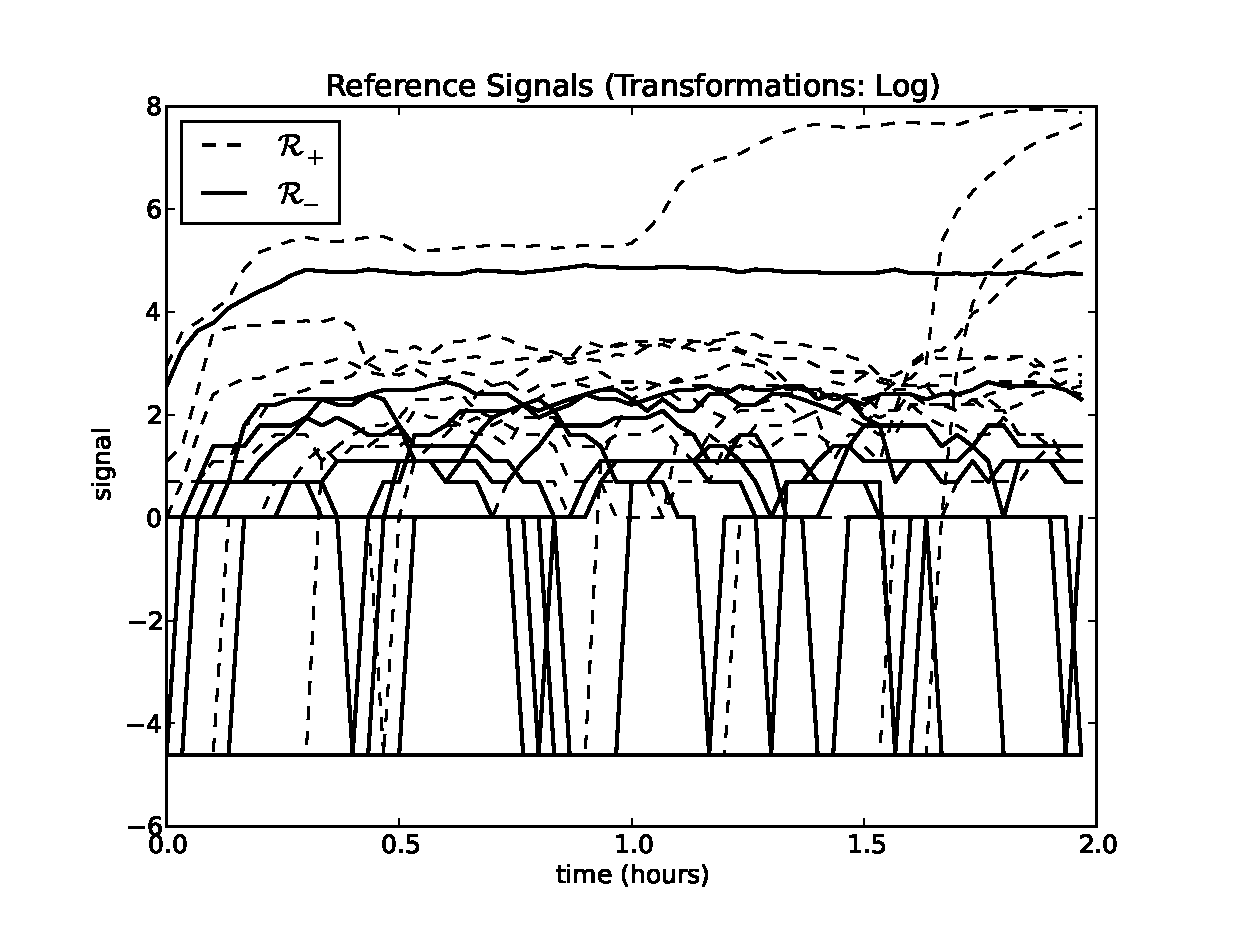
\includegraphics[width=3.10in]{../fig/final/signal_transform/log.eps}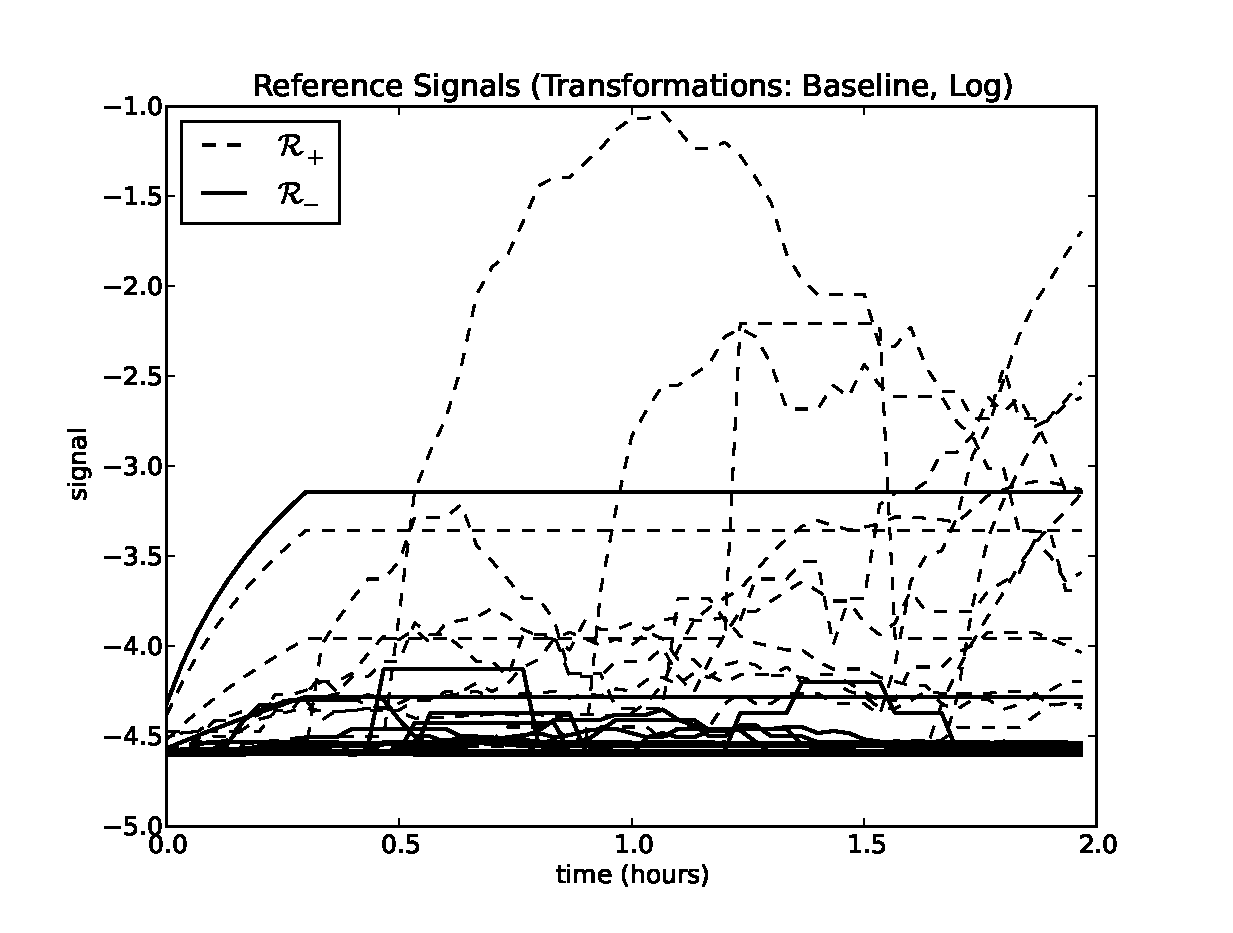
\includegraphics[width=3.10in]{../fig/final/signal_transform/log_baseline.eps}
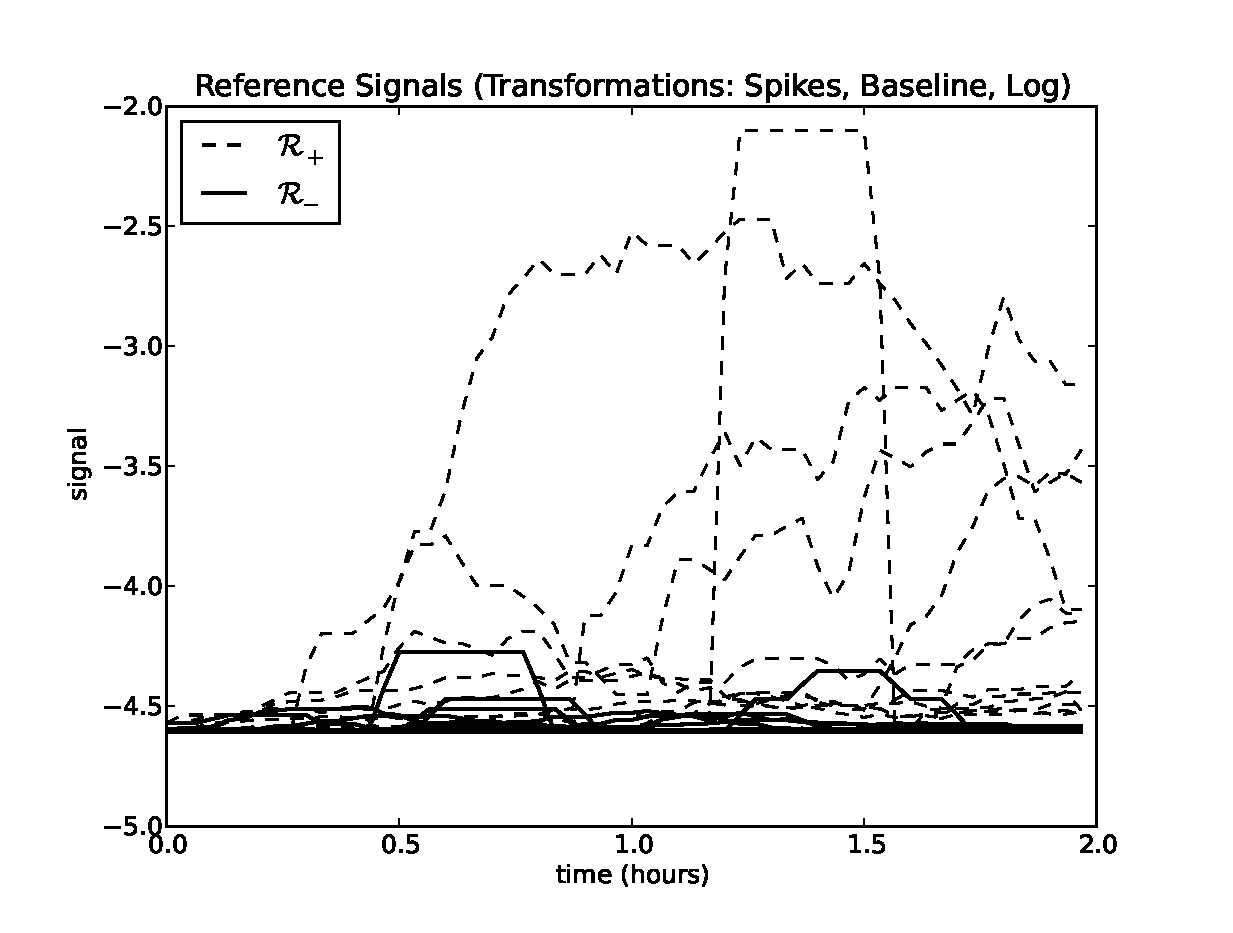
\includegraphics[width=3.10in]{../fig/final/signal_transform/log_baseline_spikes.eps}
\end{center}
\caption{\label{fig:baseline_spikes} Reference signals of either class are hard to tell apart without normalization. {\bf Top left}: no baseline or spike normalization. {\bf Top right}: Baseline normalization. {\bf Bottom}: Baseline and spike-based normalization.}
\end{figure}

\begin{figure}[h!]
\begin{center}
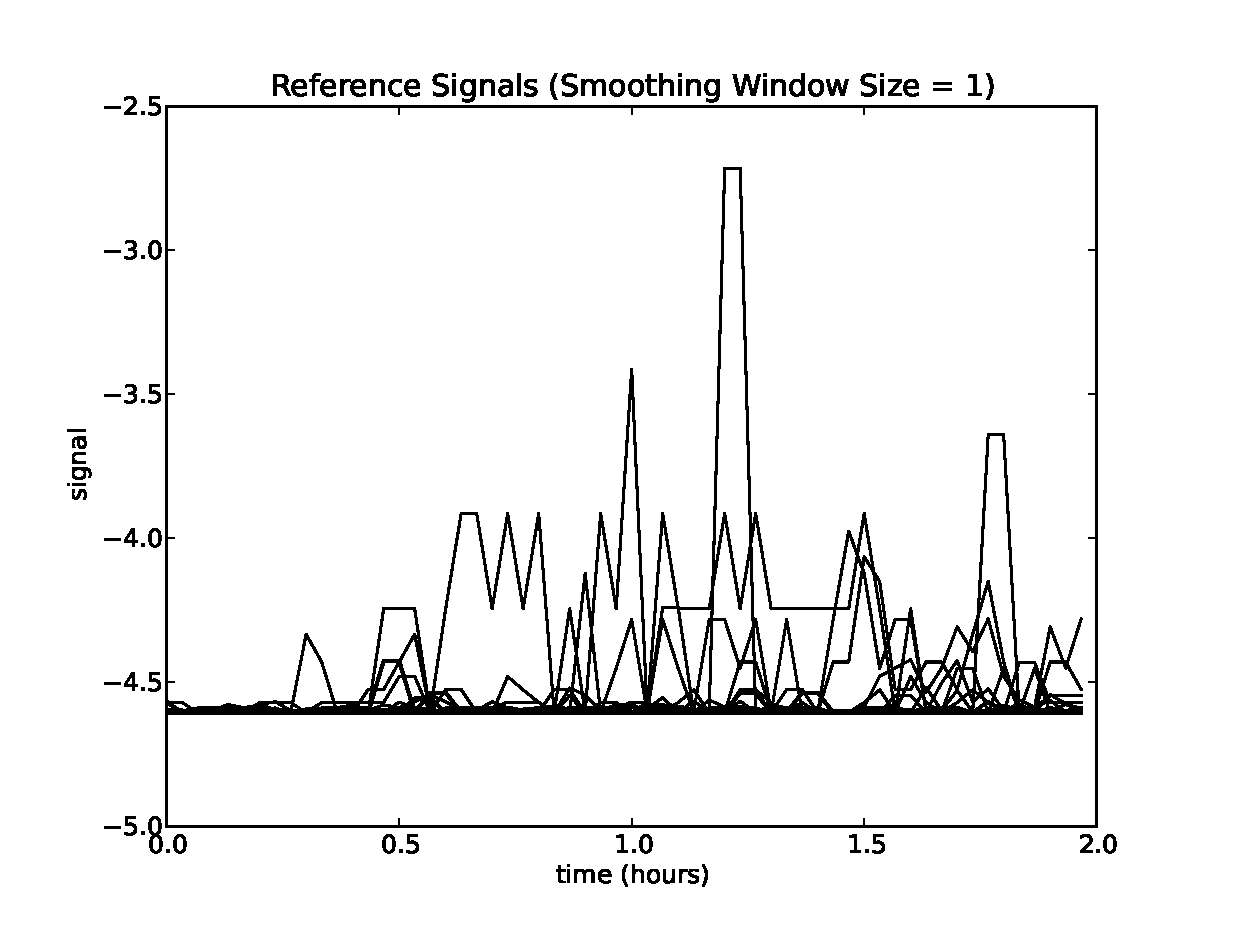
\includegraphics[width=3.10in]{../fig/final/signal_transform/smooth_1.eps}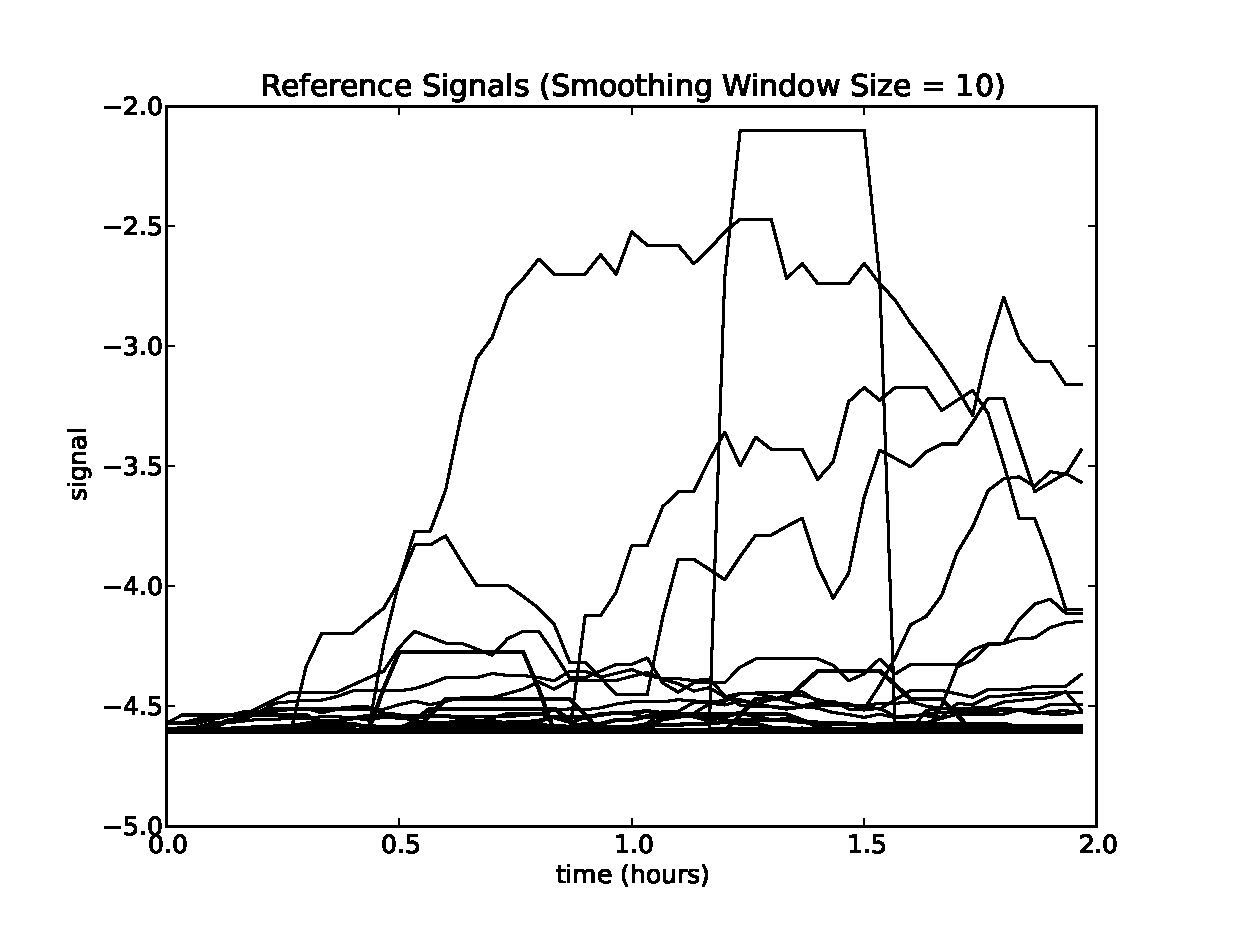
\includegraphics[width=3.10in]{../fig/final/signal_transform/smooth_10.eps}
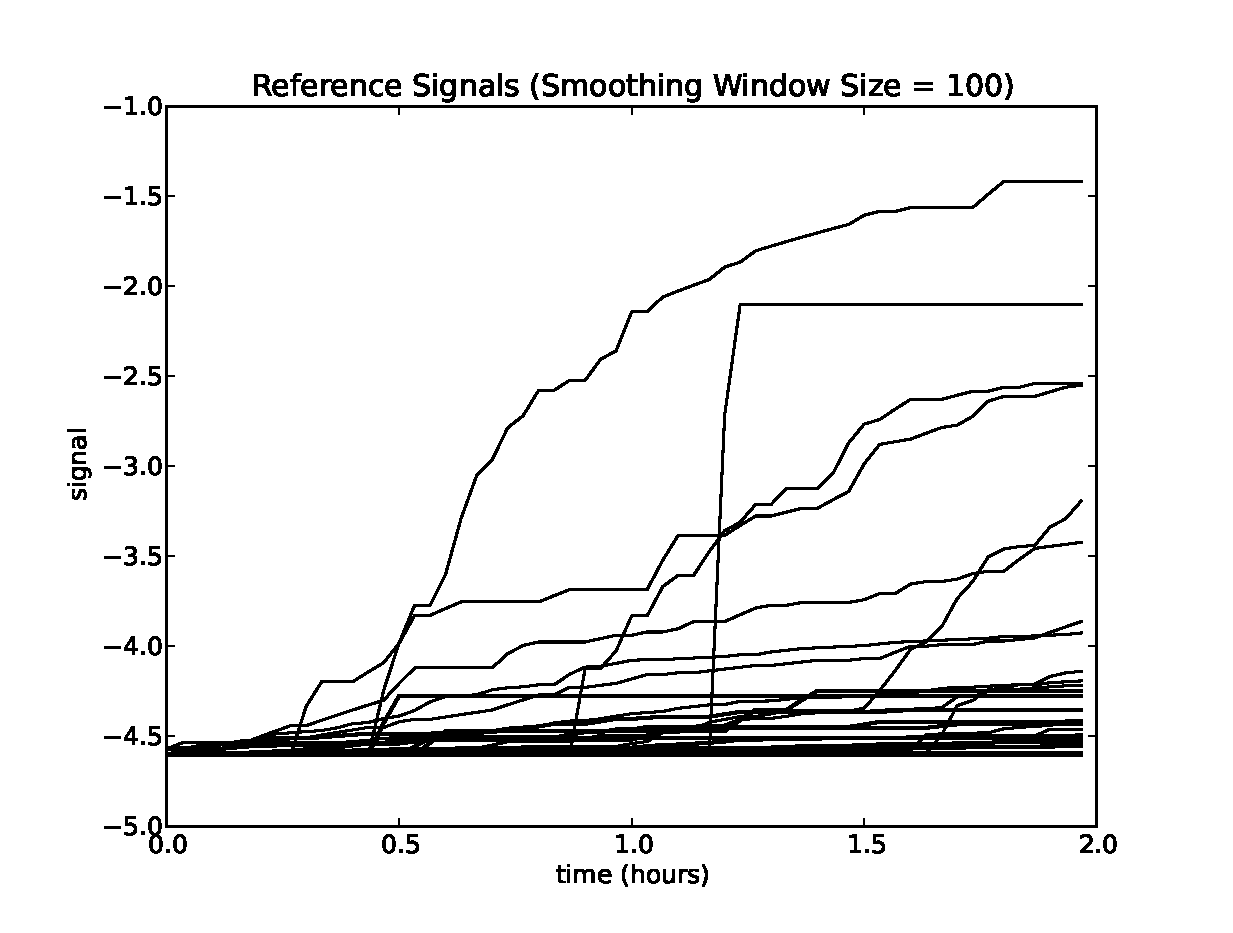
\includegraphics[width=3.10in]{../fig/final/signal_transform/smooth_100.eps}
\end{center}
\caption{\label{fig:smooth} The results of smoothing the reference signals (with spike and baseline normalization previously applied) with windows of size 1 (2 minutes, i.e. no smoothing), 10 (20 minutes), and 100 (3 hours, 20 minutes).}
\end{figure}

\begin{figure}[h!]
\begin{center}
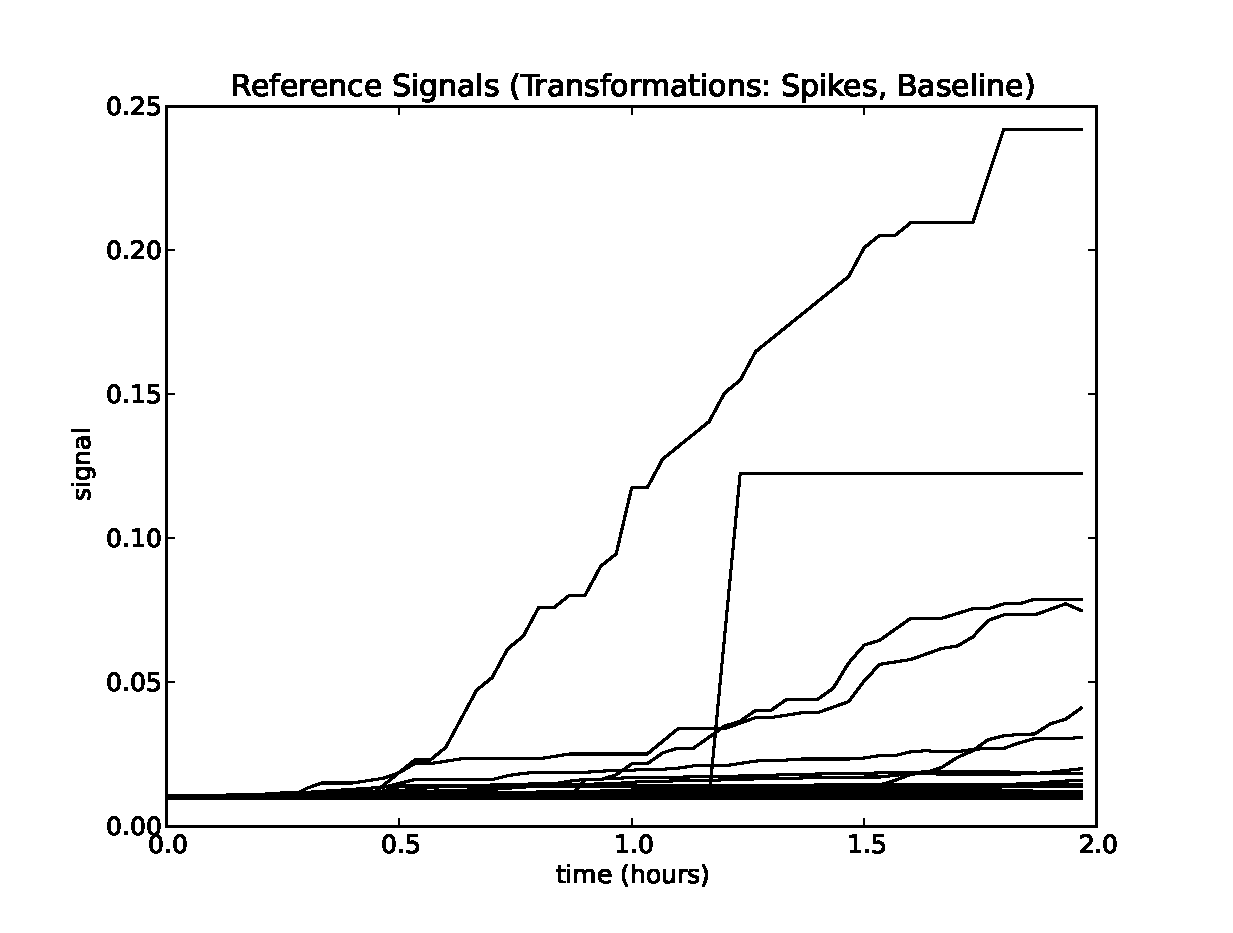
\includegraphics[width=3.10in]{../fig/final/signal_transform/no_log.eps}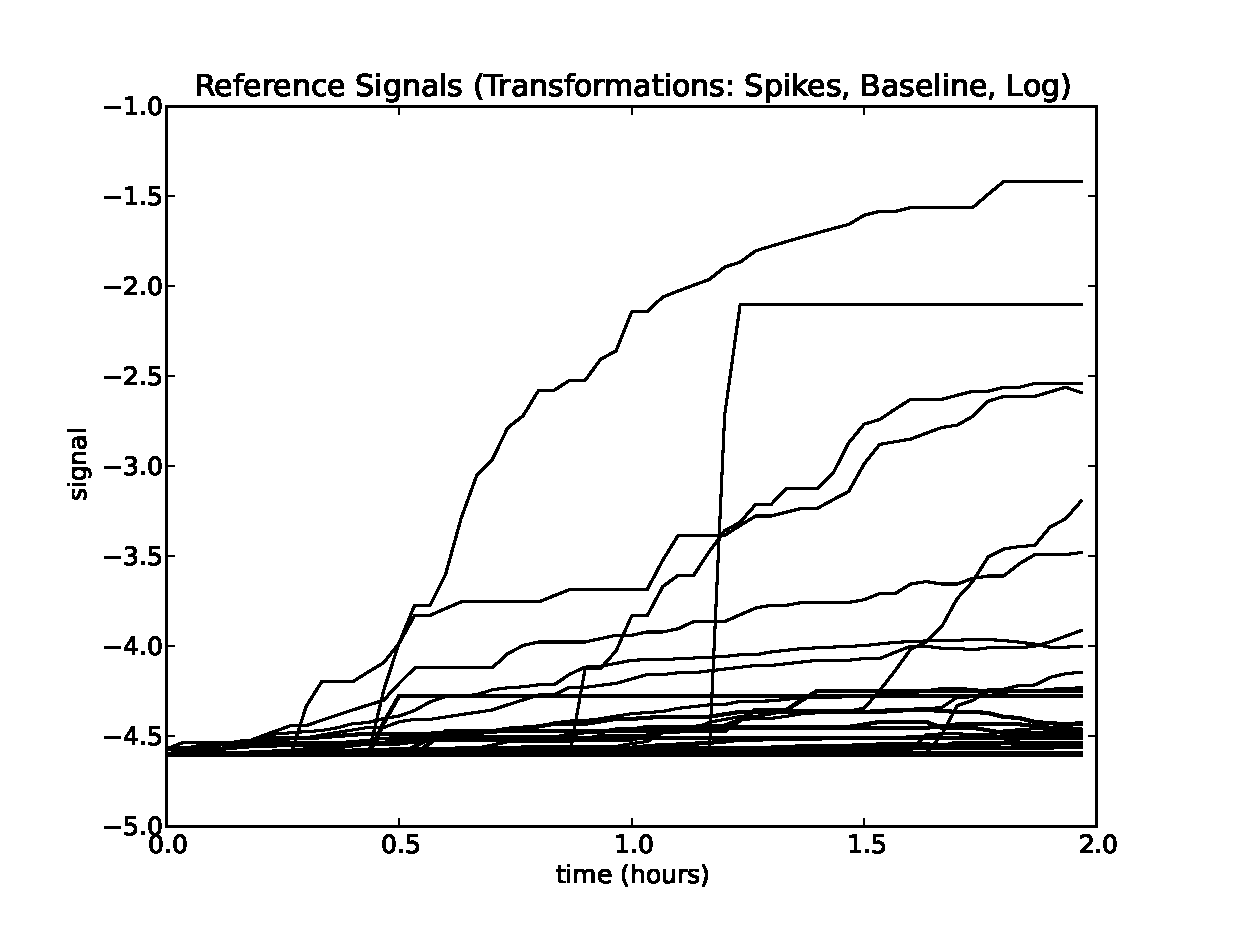
\includegraphics[width=3.1in]{../fig/final/signal_transform/yes_log.eps}
\end{center}
\caption{\label{fig:log} Logarithmically scaled reference signals (with spike and baseline normalization previously applied) allow one to make finer-grained distinctions between signals. {\bf Left}: Not logarithmically scaled. {\bf Right}: Logarithmically scaled.}
\end{figure}

\clearpage

\section{Experiment}
We propose an experiment to measure our algorithm's performance on two fronts:
error rate and relative detection time. We divide the set of topics into a
training set and a test set using a 50/50 split. For each topic in the test
set, we wish to predict if the topic will trend. If the topic really did trend,
we wish to detect it as early as possible relative to the true trend onset while
incurring minimal error.

\subsection{Detection Setup}
In principle, to test the detection algorithm, one would step through the signal
in the entire sample window for each topic in the test set and report the time
of the first detection, or that there were no detections. In practice, we take a
shortcut to avoid looking through the entire signal based on the following
observations about the activity of topics that trended and topics that did
not. First, for topics that trended, there is little, if any activity aside from
that surrounding the true onset of the trend. In the rare event that a detection
is made very far from the true onset, it is reasonable to assume that this
corresponds to a completely different event involving that topic and we can
safely ignore it. Thus, the only part of the signal worth looking at is the
signal within some time window from the true onset of the trend. Second, topics
that did not trend exhibit relatively stationary activity. That is, the signal
usually looks roughly the same over the entire sample window. Therefore, it is
reasonable to perform detection only on a piece of the signal as an
approximation to the true detection performance.

We perform detection over a window of $2N_{obs}$ samples --- twice the length of a
reference signal. For convenience and future use, we define this in terms of hours.

\begin{defn}
Let $h_{ref}$ be the number of hours corresponding to $N_{ref}$ samples. At 2 minutes per sample, $h_{ref}$ is given by $N_{ref} / 30$.
\end{defn}

For test topics that have trended, we do detection on the window spanning
$2h_{ref}$ hours centered at the true trend onset. For topics that did not
trend, we randomly choose a window of the desired size. Note that, although this
seems to require {\em a priori} knowledge of whether the test topic ever trended
or not, this is only a consequence of the shortcut we take to not do detection
over the entire sample window.

\subsection{Parameter Exploration}

\chapter{Results and Discussion}
\label{ch:results}

In this chapter, I present the results of the trend detection experiment
described in chapter \ref{ch:data}. I show the quality of the trend detection
algorithm using ROC curves and distributions of detection time relative to the
true trend onset. I analyze the effect of the algorithm parameters on the
tradeoff between false positive rate, true positive rate, and relative detection
time. Finally, I propose parameter regimes appropriate for three situations: 1)
the cost of a false positive outweighs the cost of a false negative, 2) the cost
of a false negative outweighs the cost of a false positive, and 3) the costs of
a false positive and a false negative are comparable.

\section{ROC Curve Envelopes}

Figures \ref{fig:roc_env1} and \ref{fig:roc_env2} shows the false positive
rates ($FPR$) and true positive rates ($TPR$) that result from varying each
detection parameter, aggregated over all combinations of the remaining
parameters. The left side of each plot shows a scatter plot of false positive
and true positive rates, while the right side shows the upper-left-most envelope
of the set of all ROC curves.

\begin{figure}[!h]
\begin{center}
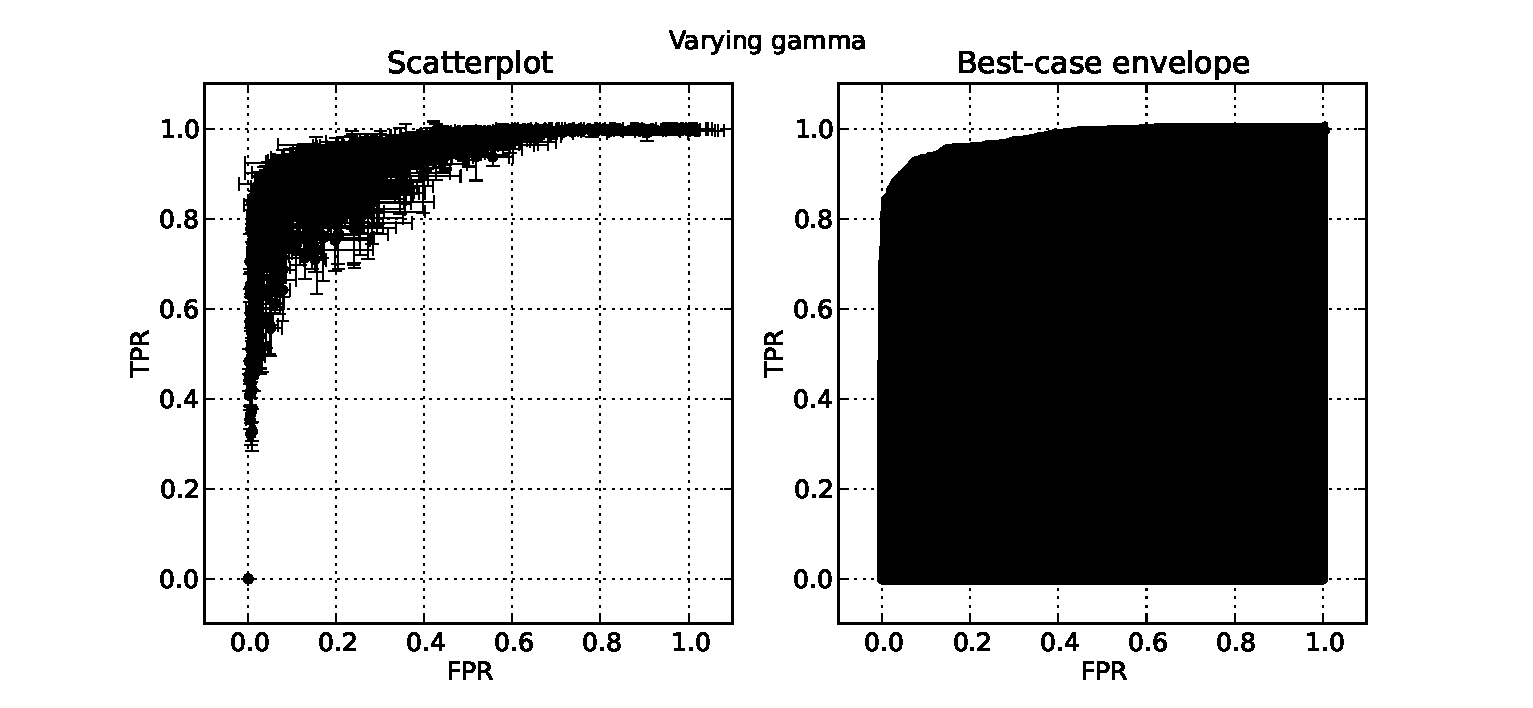
\includegraphics[height=2.5in]{../fig/final/scatter_env/gamma}
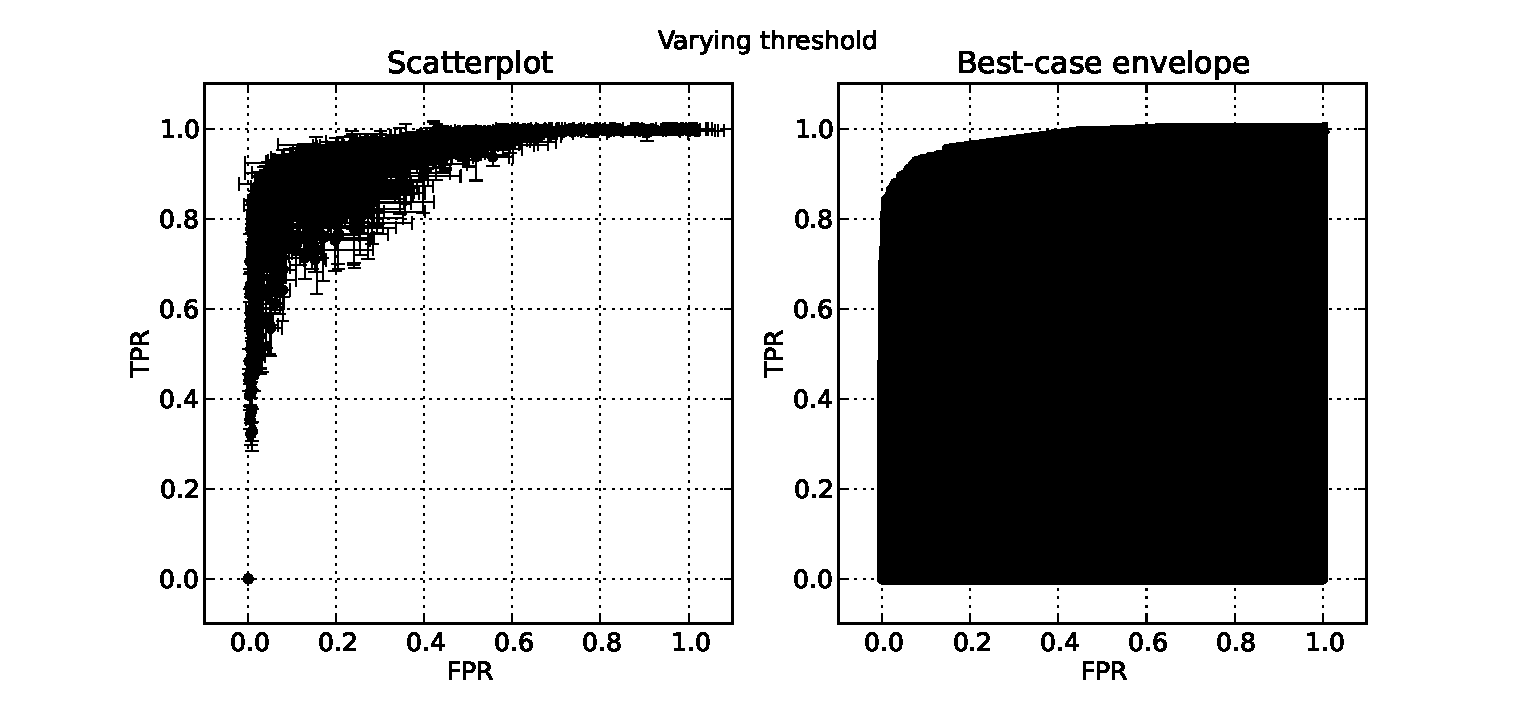
\includegraphics[height=2.5in]{../fig/final/scatter_env/threshold}
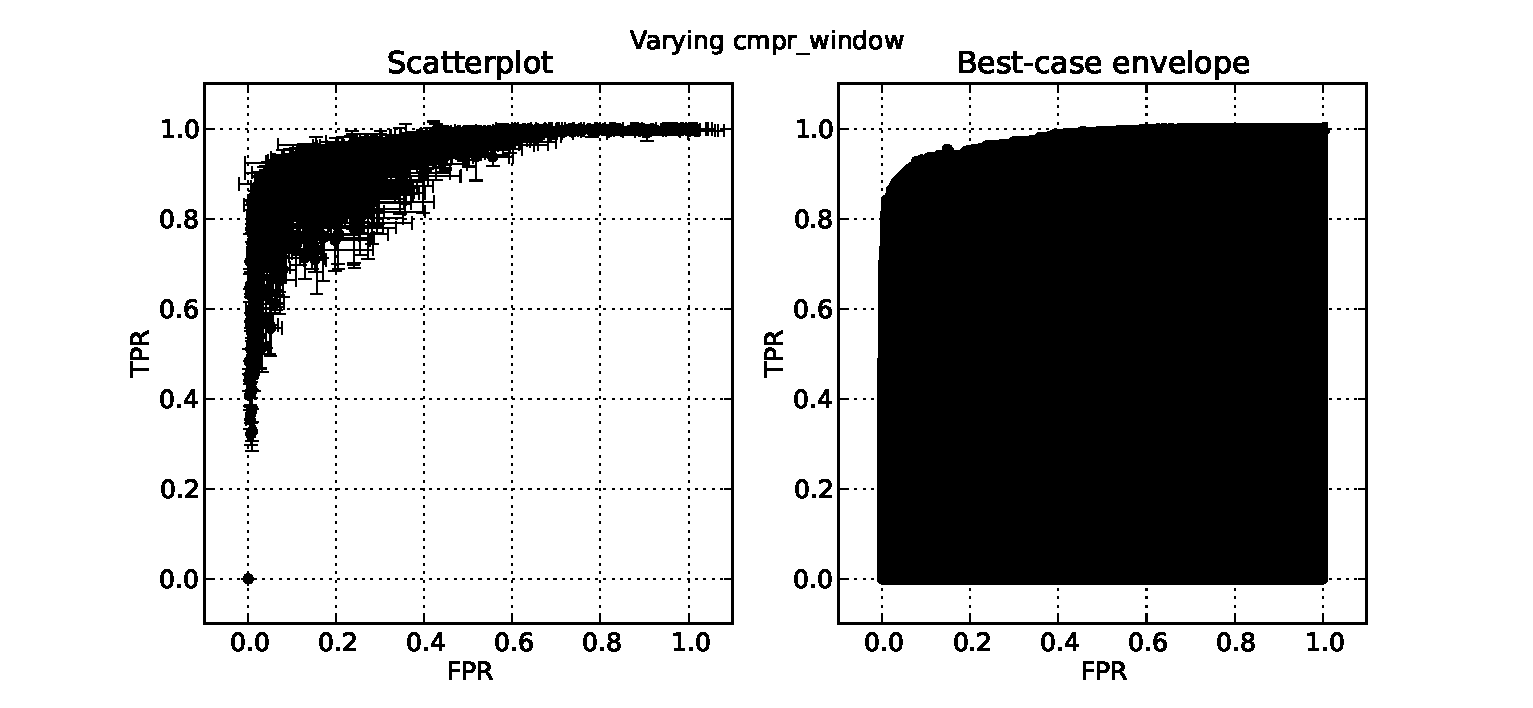
\includegraphics[height=2.5in]{../fig/final/scatter_env/cmpr_window}
\end{center}
\caption{\label{fig:roc_env2}}
\end{figure}

\begin{figure}[!h]
\begin{center}
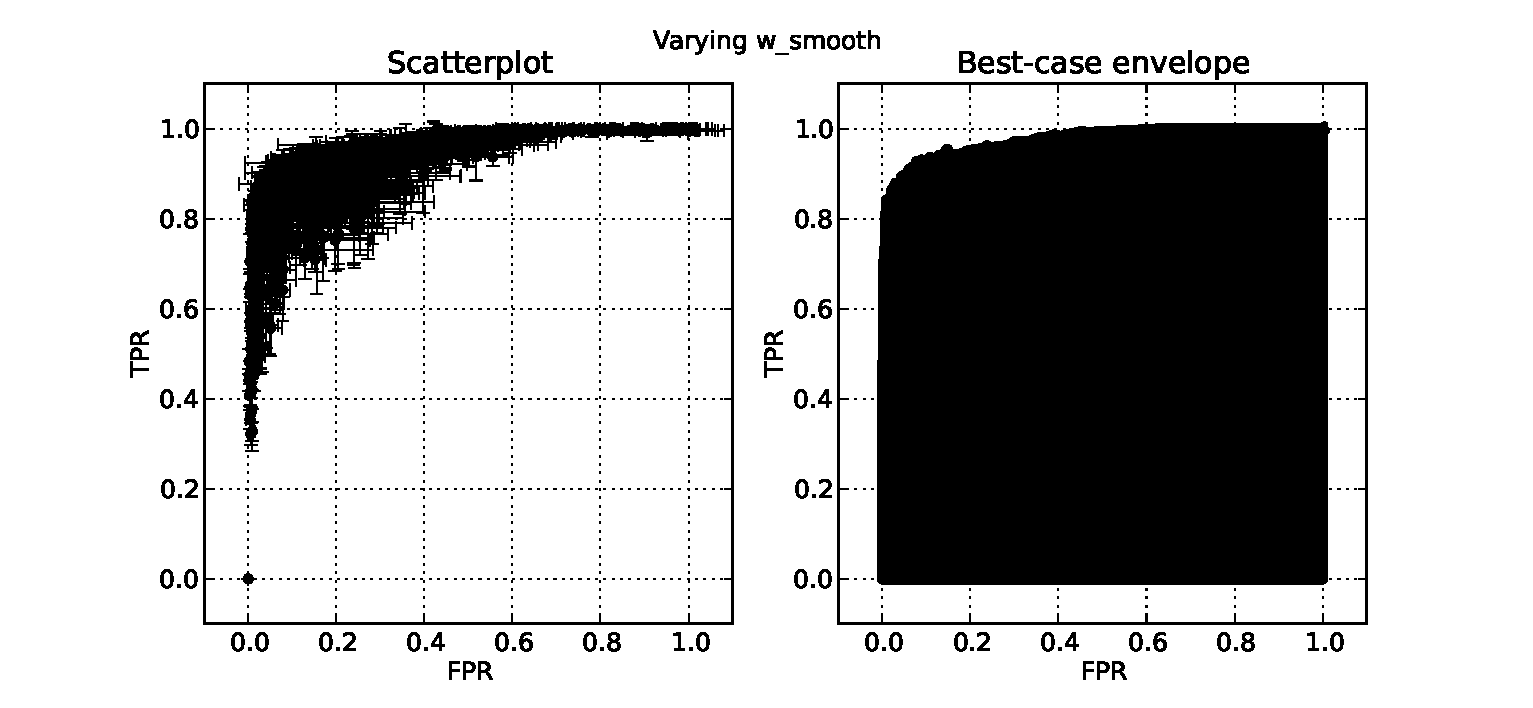
\includegraphics[height=2.5in]{../fig/final/scatter_env/w_smooth}
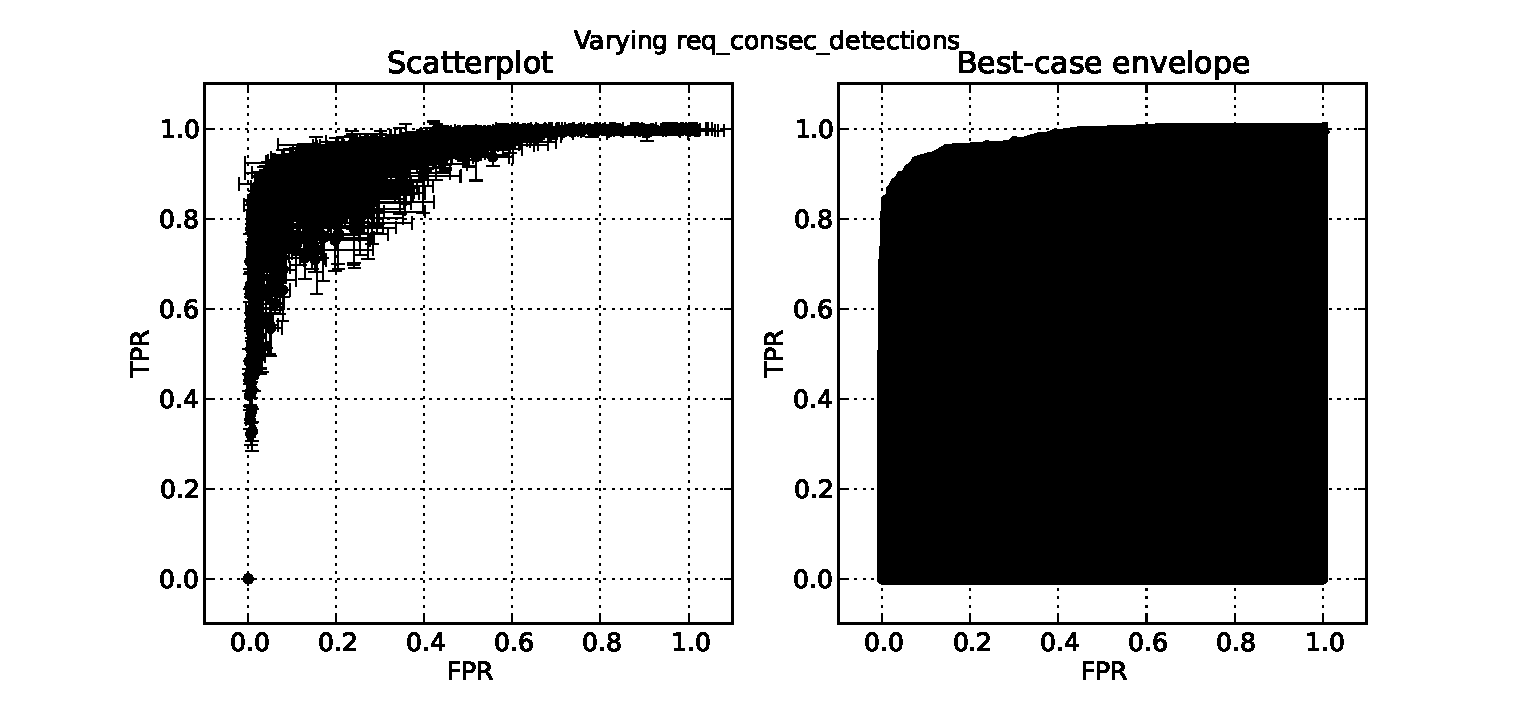
\includegraphics[height=2.5in]{../fig/final/scatter_env/req_consec_detections}
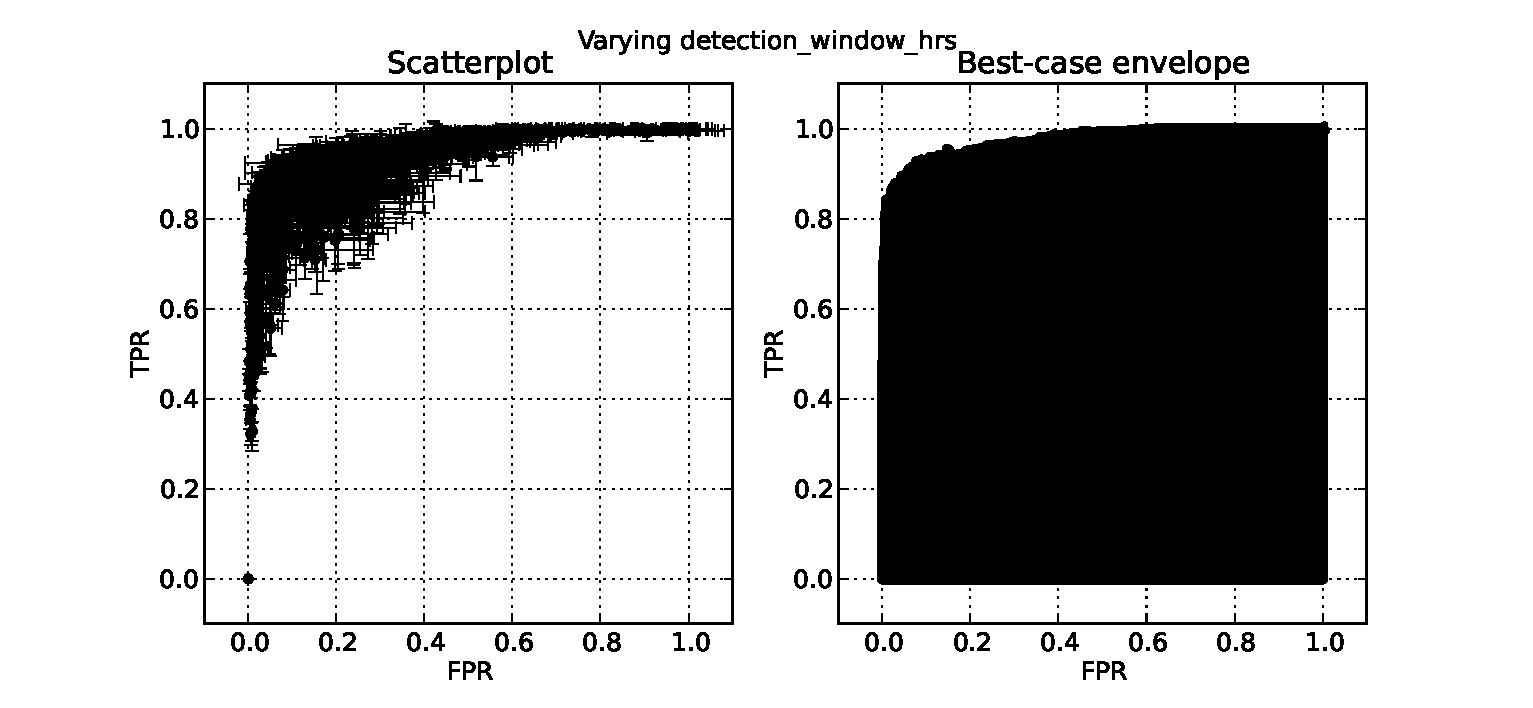
\includegraphics[height=2.5in]{../fig/final/scatter_env/detection_window_hrs}
\end{center}
\caption{\label{fig:roc_env1}}
\end{figure}


\section{Examples} %TODO: Call this something better

True positives. Slow rising vs fast rising.

True negatives.

False positives. Stuff with significant volume or spikes.

False negatives. Stuff with too little volume or not enough spikes.

\section{Effect of Parameters}

Do we move up or down the curve?

We show how varying a given parameter $p$ trades off $FPR$ for $TPR$ by
computing the discrete derivative of $FPR$ and $TPR$ with respect to $p$. For
each ROC curve, corresponding to the variable parameter $p$ and some fixed
combination of remaining parameters, we compute
\begin{gather}
\Delta_{p,i}^{FPR} = \frac{FPR(p_{i}) - FPR(p_{i-1})}{p_i - p_{i-1}}\\
\Delta_{p,i}^{TPR} = \frac{TPR(p_{i}) - TPR(p_{i-1})}{p_i - p_{i-1}}
\end{gather}
for each ROC curve associated with $p$ and for $i$ ranging from the second to the last value
of $p$ in increasing order. If each point on the ROC curve is produced by
multiple trials, we compute the above for all possible combinations of ROC
curves. Finally, we compute the above across all combinations of fixed
parameters.

The result is a distribution of discrete derivatives of $FPR$ and $TPR$ with
respect to a variable parameter of interest $p$ which highlights the effect of
$p$ on tradeoffs between $FPR$ and $TPR$. We can refer this effect as moving
``up'' the ROC curve, or ``down'' the ROC curve. If most of the mass of
$\Delta_{p}^{FPR}$ and $\Delta_{p}^{TPR}$ is at values greater than 0, then an
increase in $p$ causes a decrease in $FPR$ at the expense of lower $TPR$, moving
down the curve. If, on the other hand, most of the mass is at values less than
zero, an increase in $p$ causes an increase in $TPR$ at the expensive of higher
$FPR$, moving up the curve.

Figure \ref{fig:deltas} shows this effect for each parameter.

\begin{figure}[!h]
\begin{center}
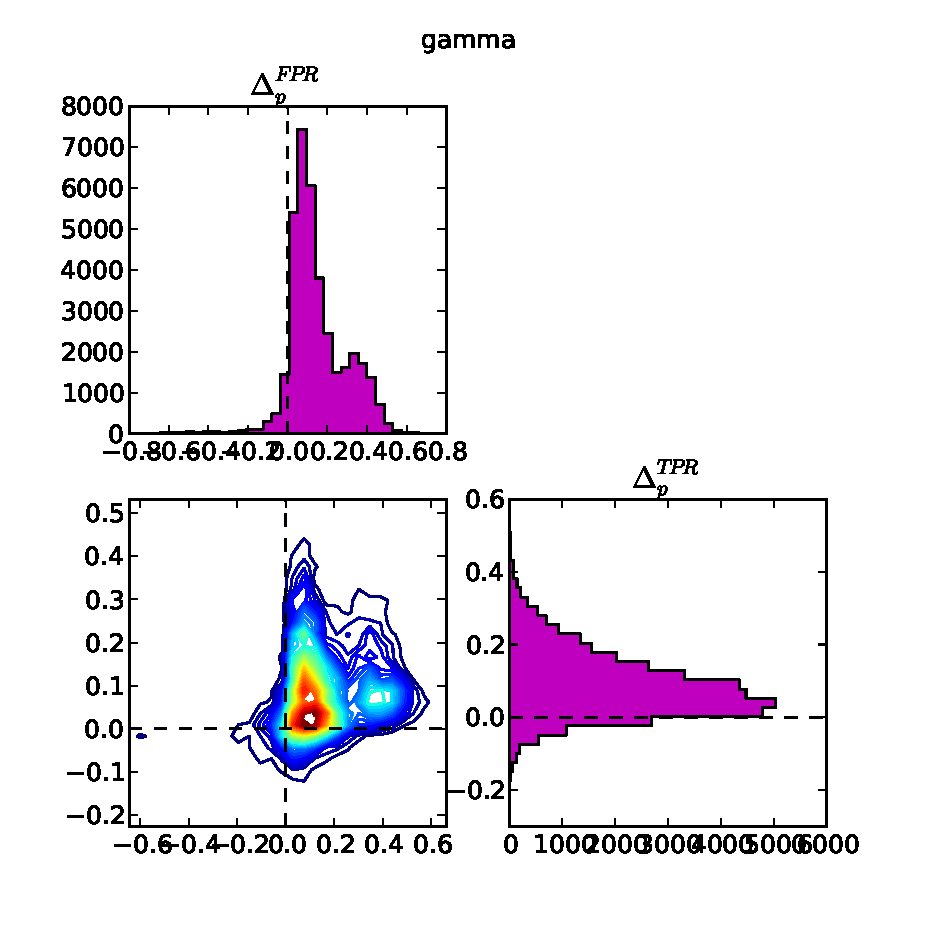
\includegraphics[width=4in]{../fig/final/delta_hist/gamma}
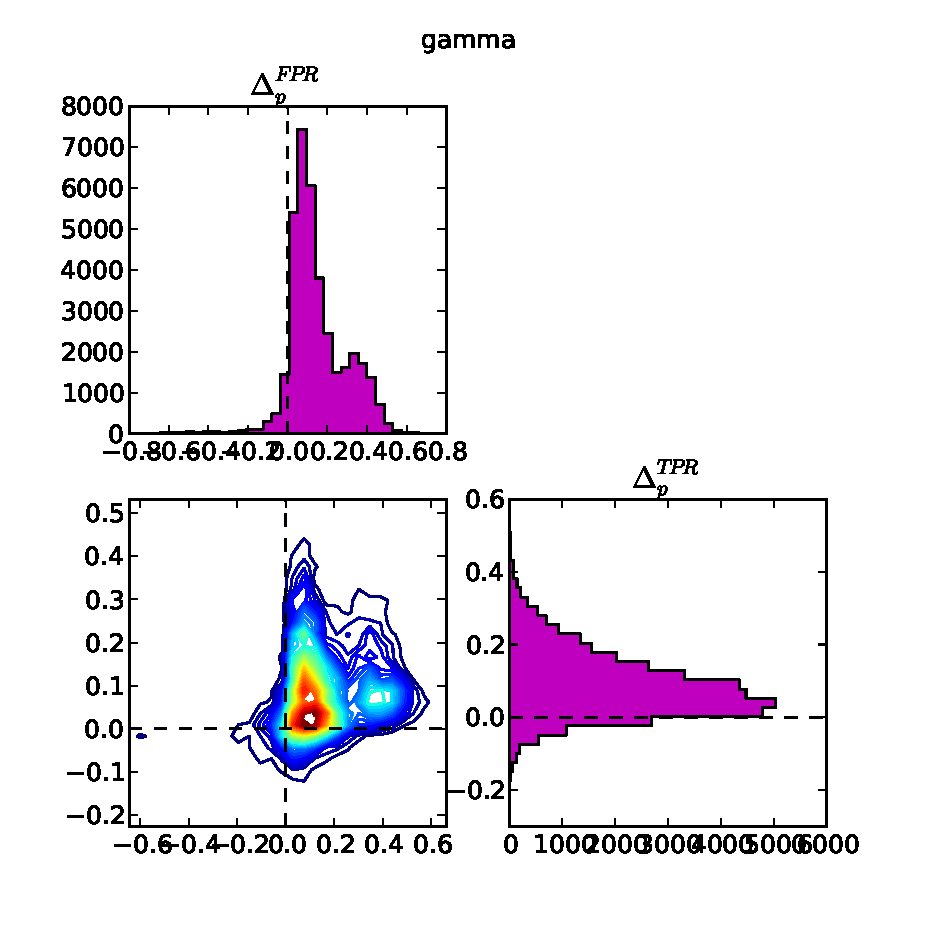
\includegraphics[width=4in]{../fig/final/delta_hist/gamma}
\end{center}
\caption{\label{fig:deltas1}}
\end{figure}

\begin{figure}[!h]
\begin{center}
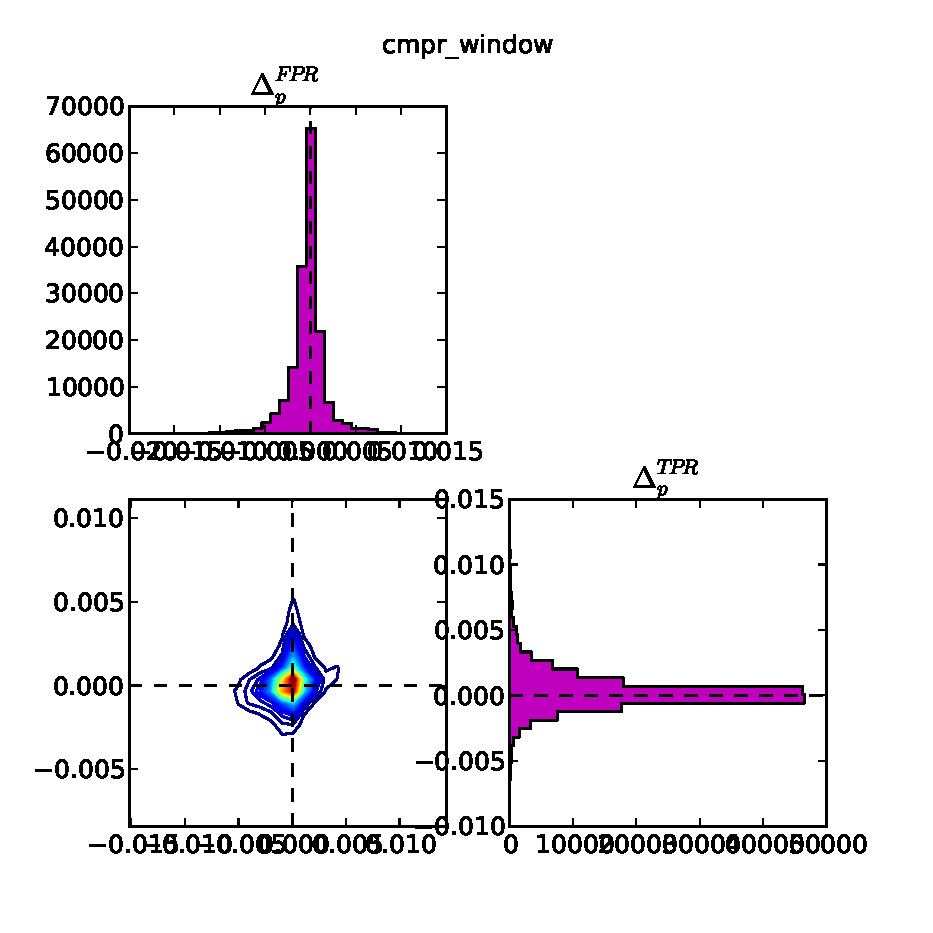
\includegraphics[width=4in]{../fig/final/delta_hist/cmpr_window}
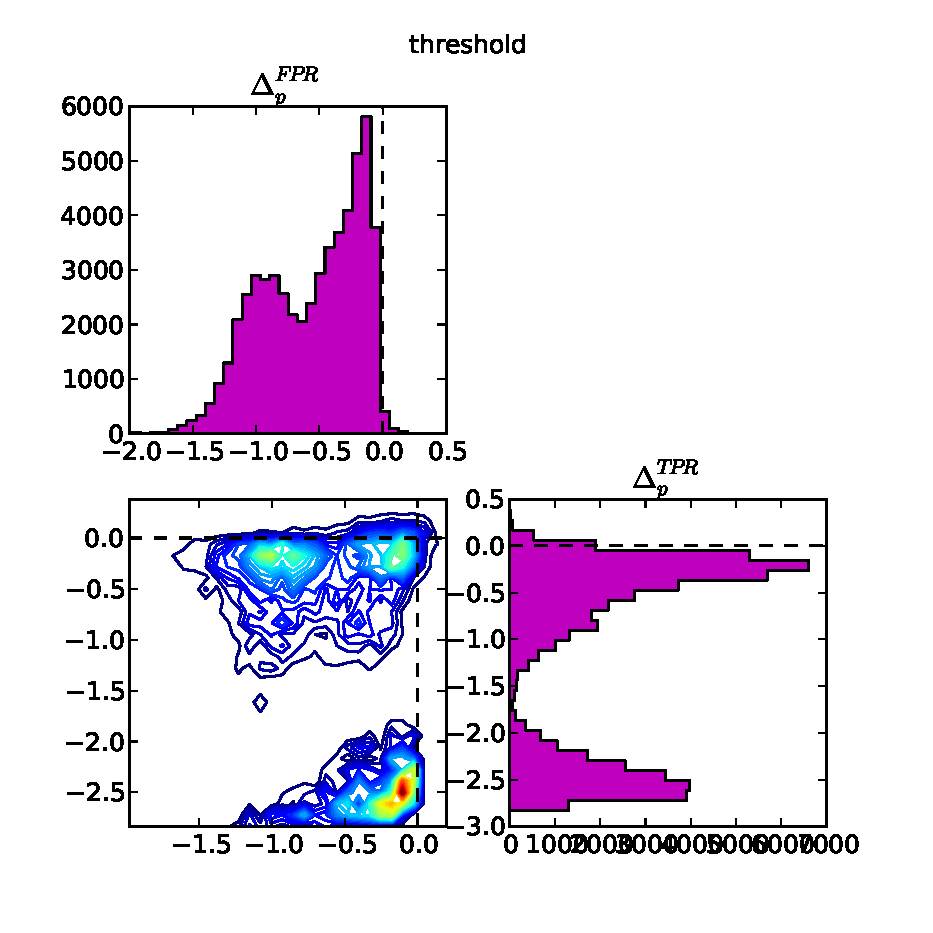
\includegraphics[width=4in]{../fig/final/delta_hist/threshold}
\end{center}
\caption{\label{fig:deltas2}}
\end{figure}

\begin{figure}[!h]
\begin{center}
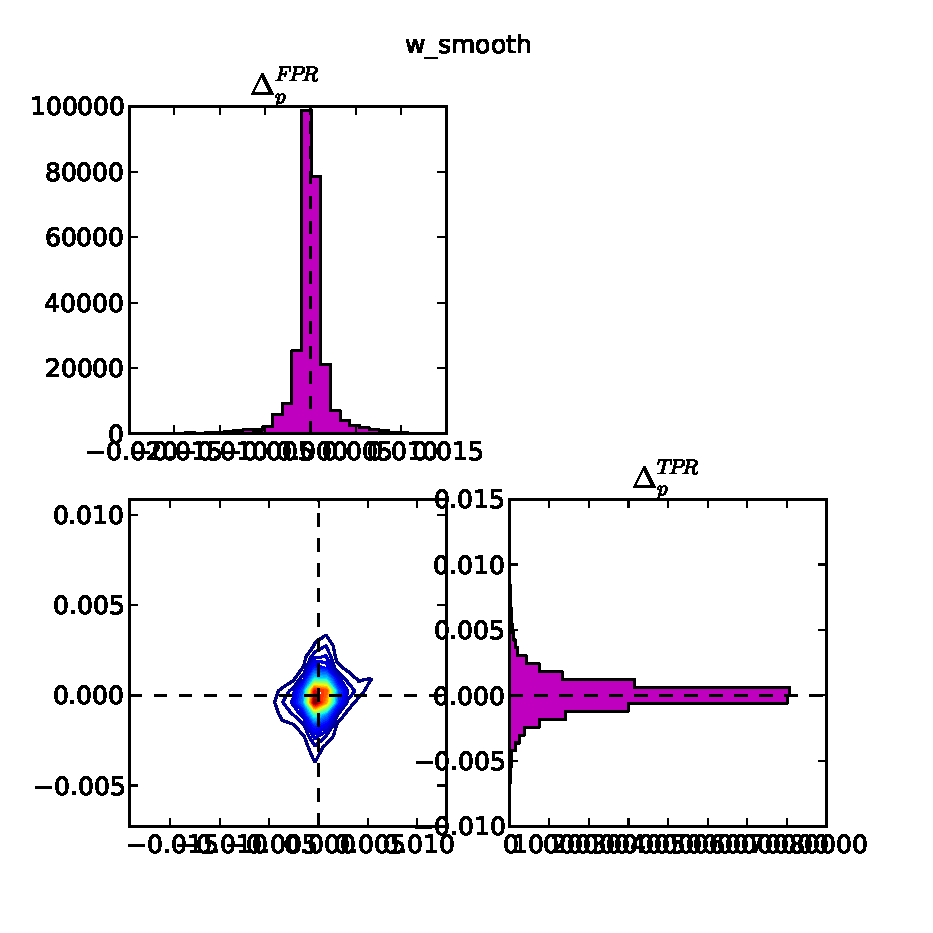
\includegraphics[width=4in]{../fig/final/delta_hist/w_smooth}
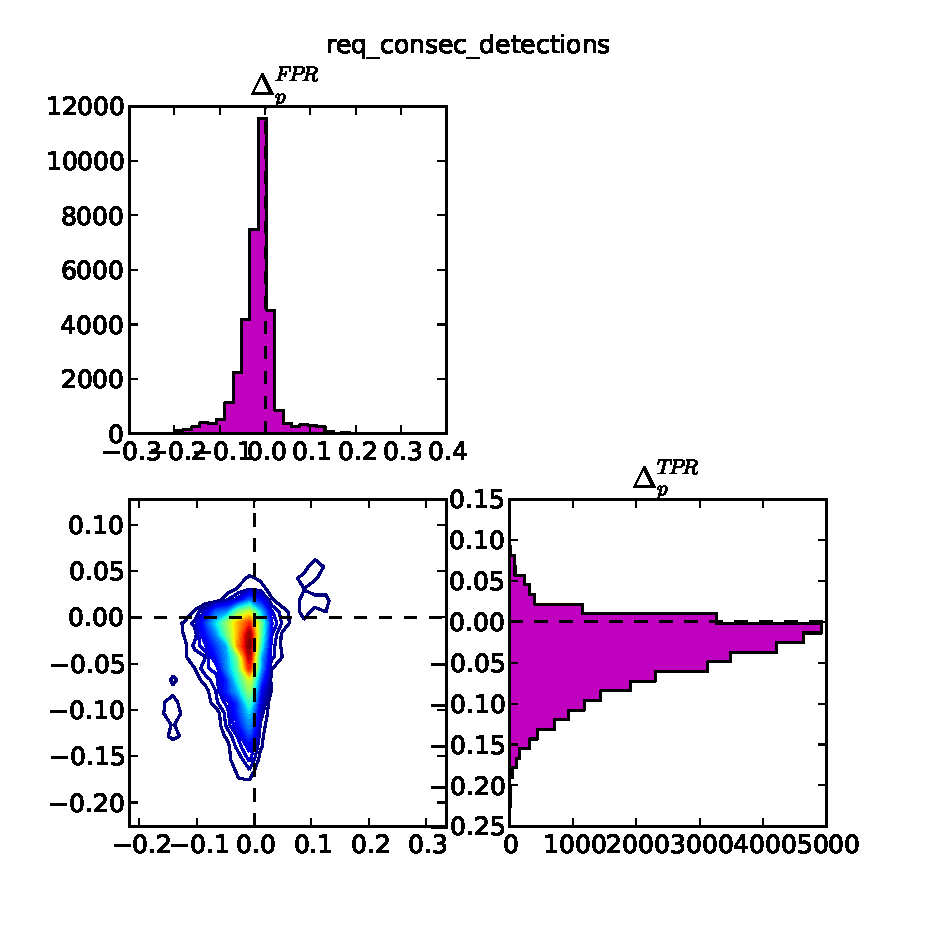
\includegraphics[width=4in]{../fig/final/delta_hist/req_consec_detections}
\end{center}
\caption{\label{fig:deltas3}}
\end{figure}

% TODO: Figure

% TODO: consistent effect, vs contingent effect
It is clear that varying some parameters has the same effect regardless of the
remaining parameters, at least within the range of values explored. 


%TODO: Delta histograms

Increasing \vt{Gamma} always moves us up the curve.
Increasing \vt{Threshold} always moves us down the curve.
Increasing \vt{ReqConsecDetections} always moves us down the curve.

\begin{figure}[!h]
\begin{center}
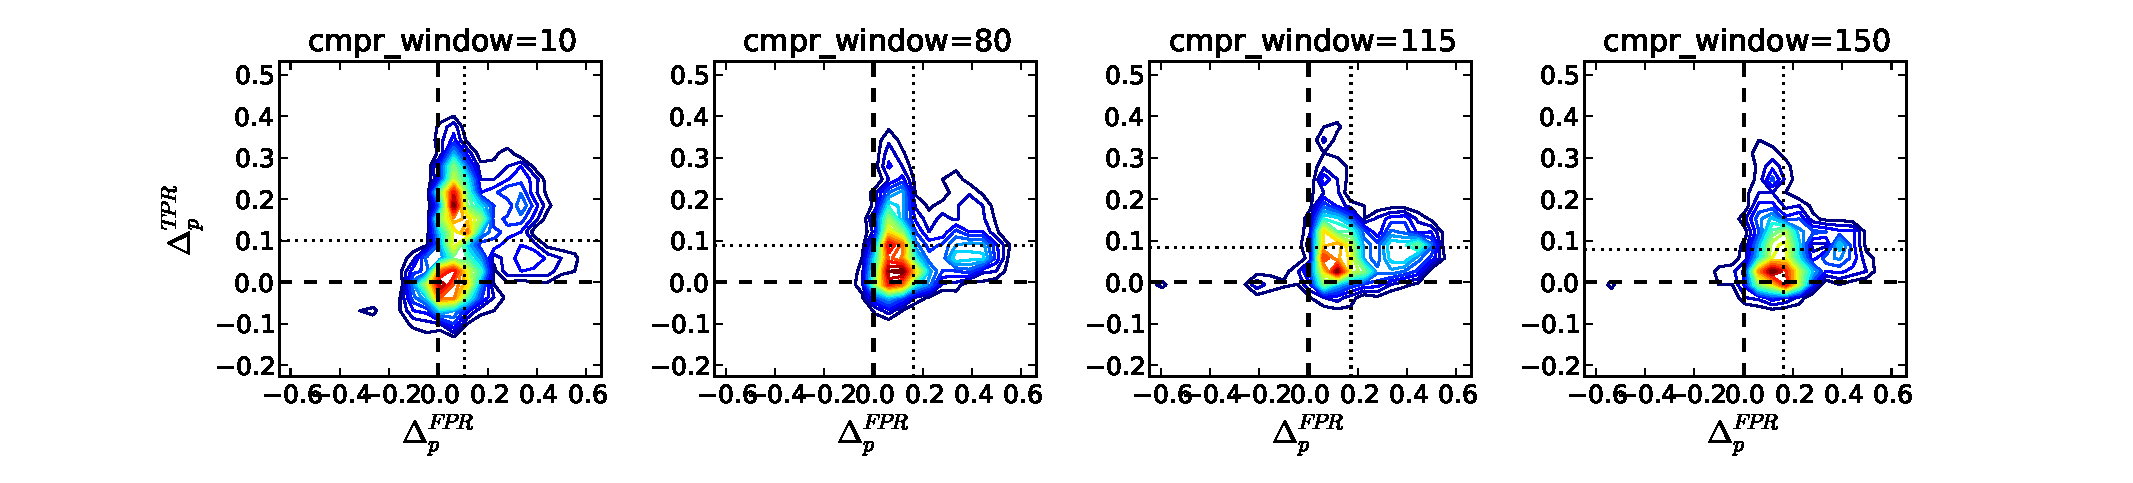
\includegraphics[height=1.5in]{../fig/final/delta_hist_sec/gamma/cmpr_window}
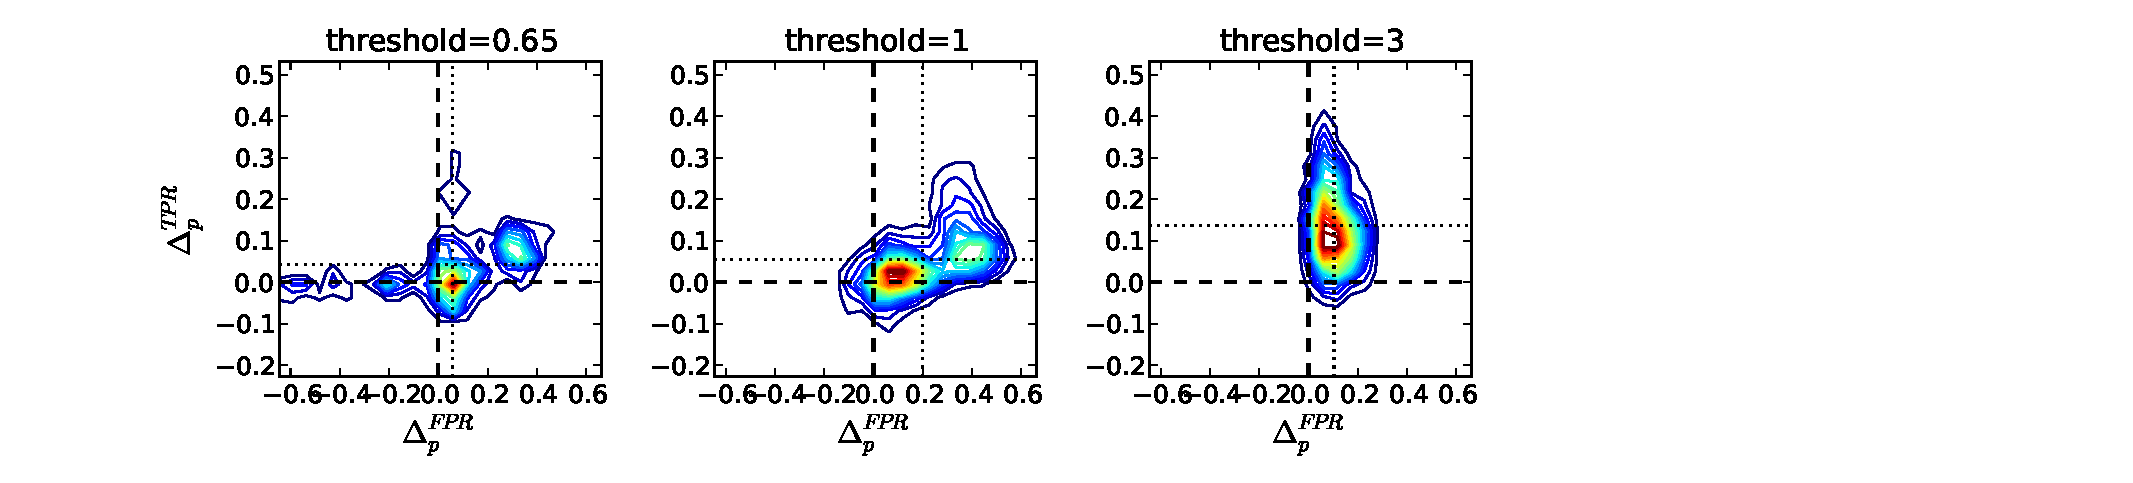
\includegraphics[height=1.5in]{../fig/final/delta_hist_sec/gamma/threshold}
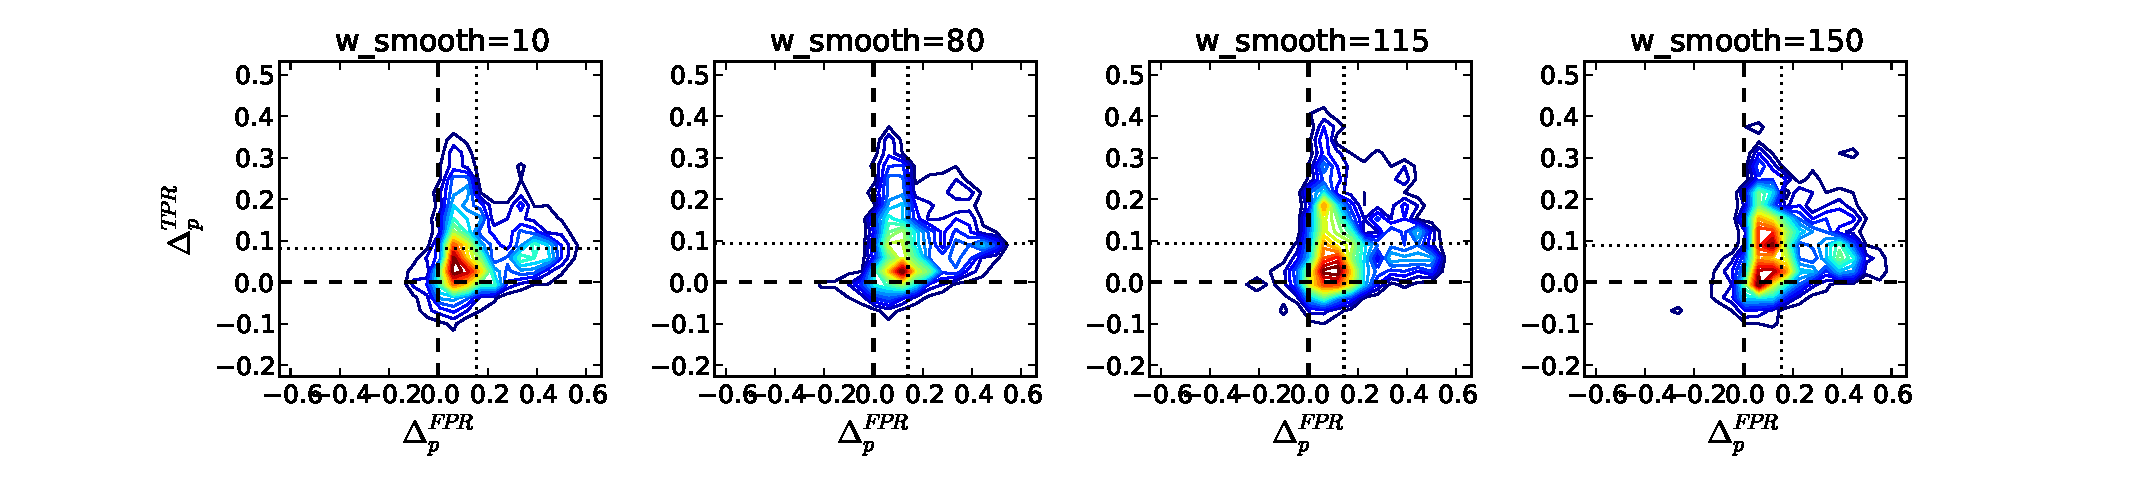
\includegraphics[height=1.5in]{../fig/final/delta_hist_sec/gamma/w_smooth}
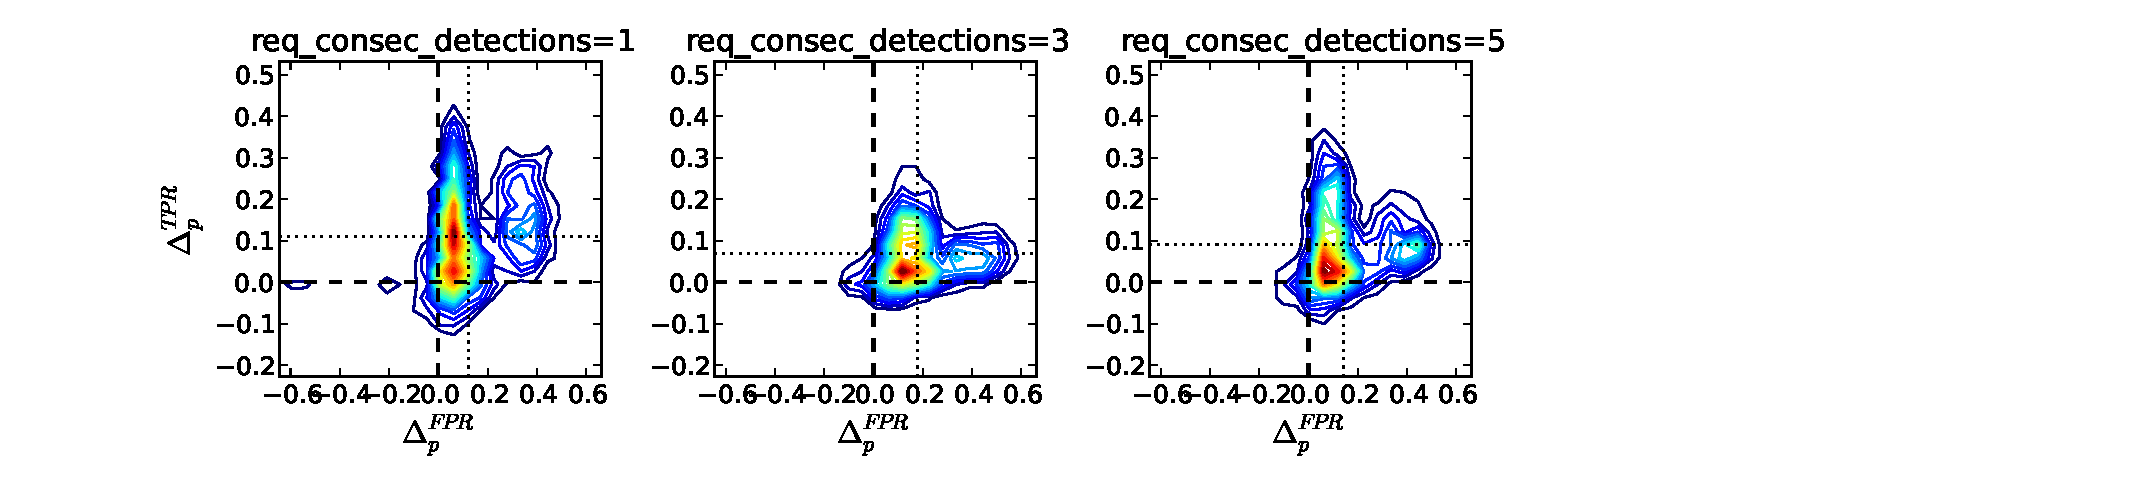
\includegraphics[height=1.5in]{../fig/final/delta_hist_sec/gamma/req_consec_detections}
\end{center}
\caption{\label{fig:delta_sec1} Secondary effects of parameters for a varying \vt{Gamma}}
\end{figure}

\begin{figure}[!h]
\begin{center}
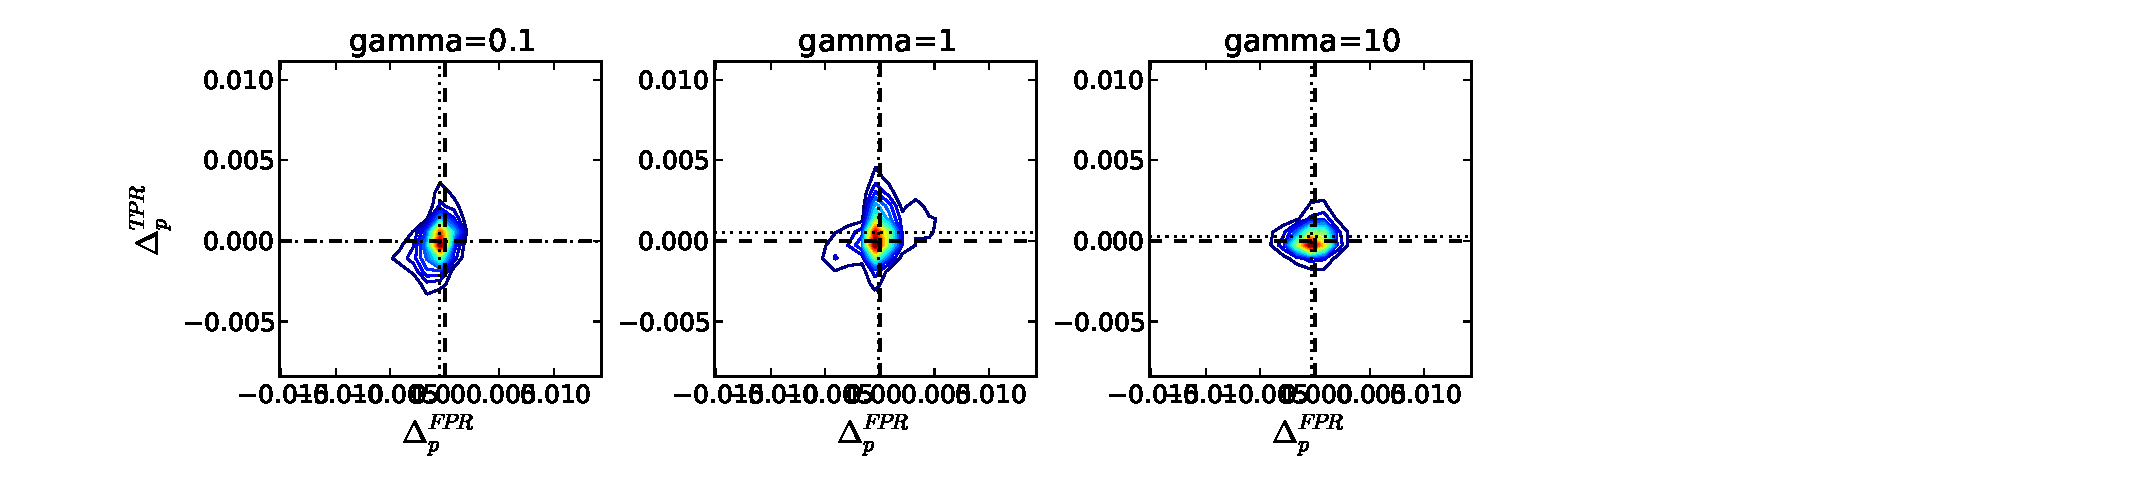
\includegraphics[height=1.5in]{../fig/final/delta_hist_sec/cmpr_window/gamma}
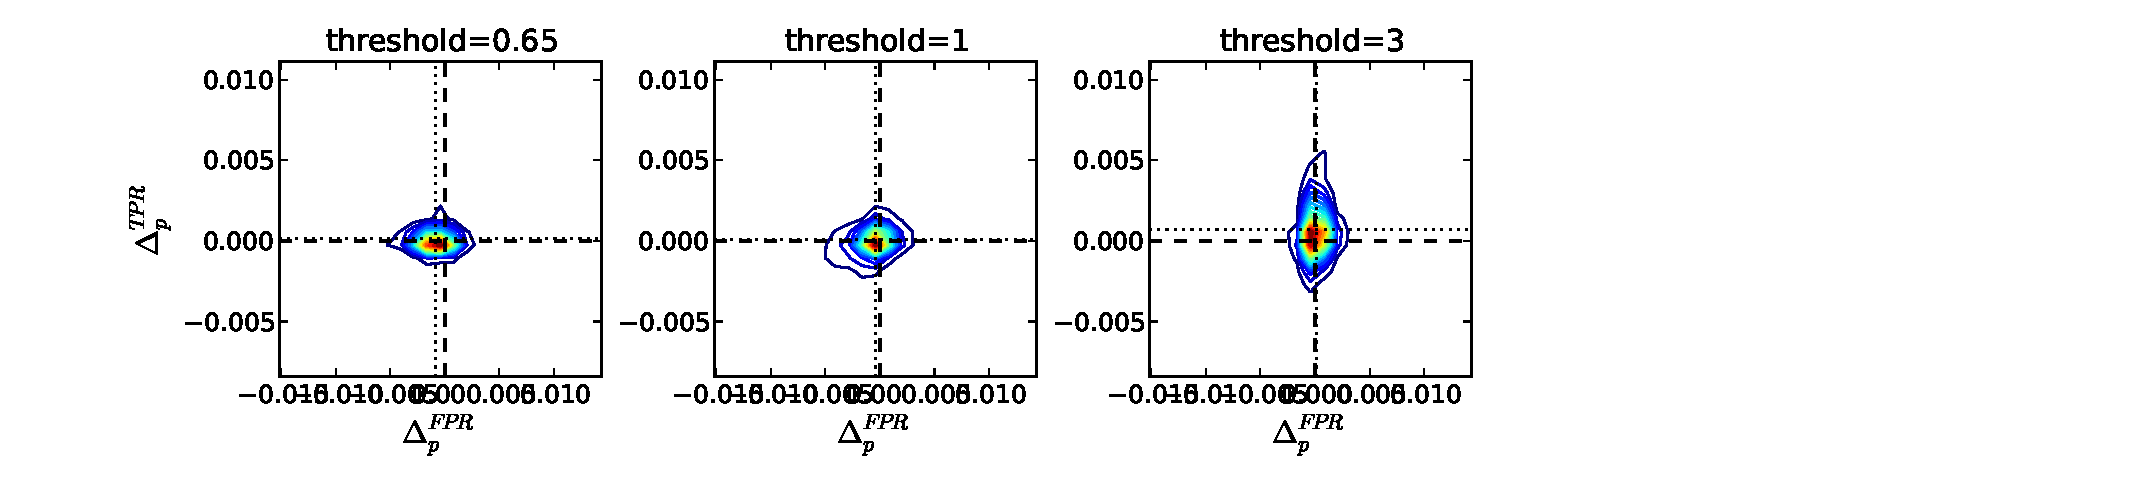
\includegraphics[height=1.5in]{../fig/final/delta_hist_sec/cmpr_window/threshold}
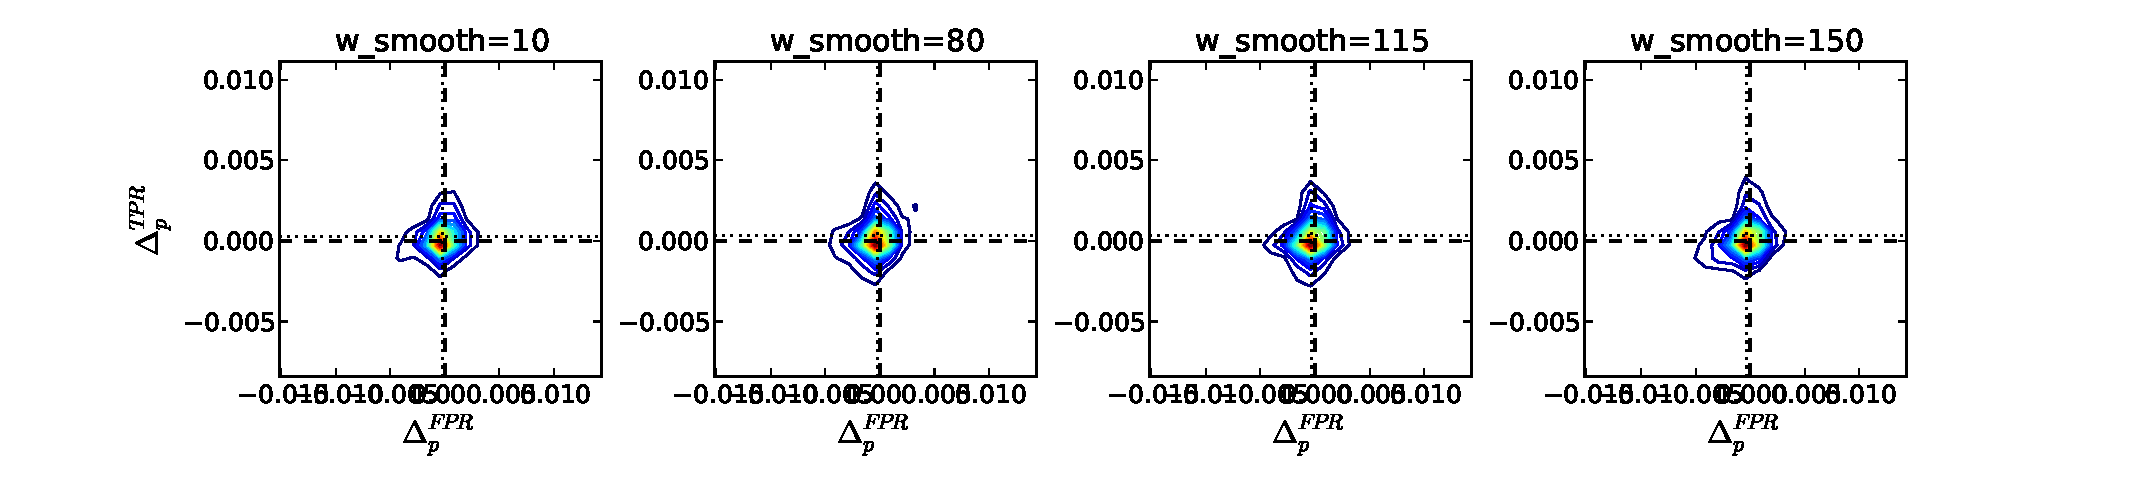
\includegraphics[height=1.5in]{../fig/final/delta_hist_sec/cmpr_window/w_smooth}
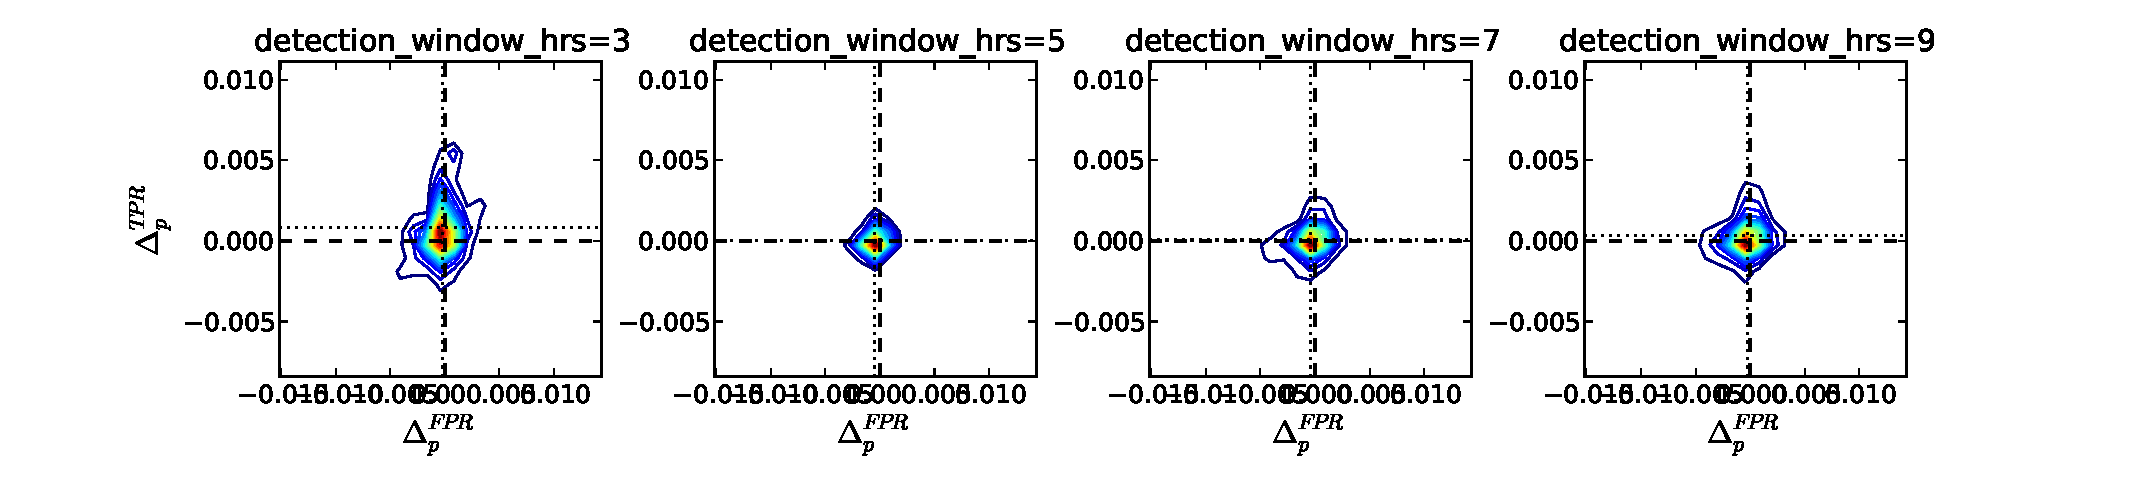
\includegraphics[height=1.5in]{../fig/final/delta_hist_sec/cmpr_window/detection_window_hrs}
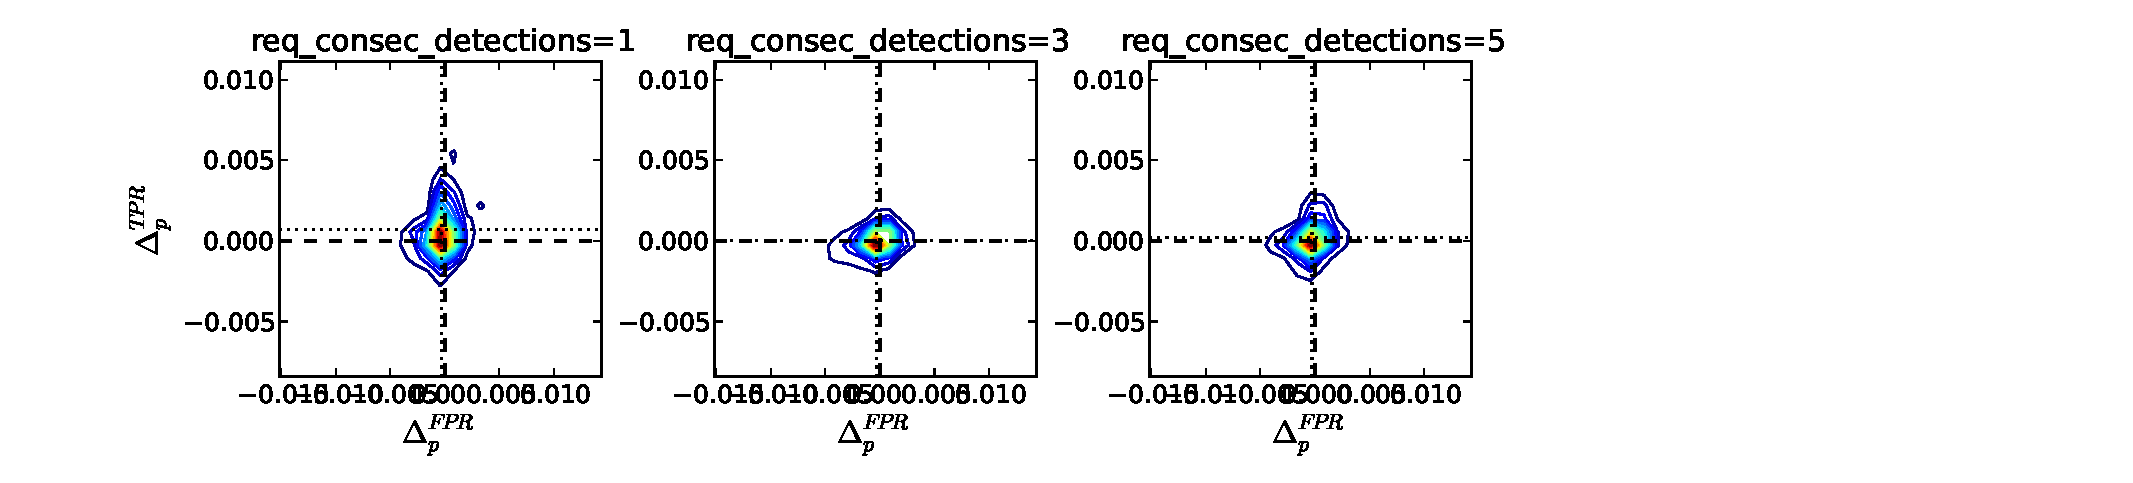
\includegraphics[height=1.5in]{../fig/final/delta_hist_sec/cmpr_window/req_consec_detections}
\end{center}
\caption{\label{fig:delta_sec2} Secondary effects of parameters for a varying \vt{CmprWindow}}
\end{figure}

\begin{figure}[!h]
\begin{center}
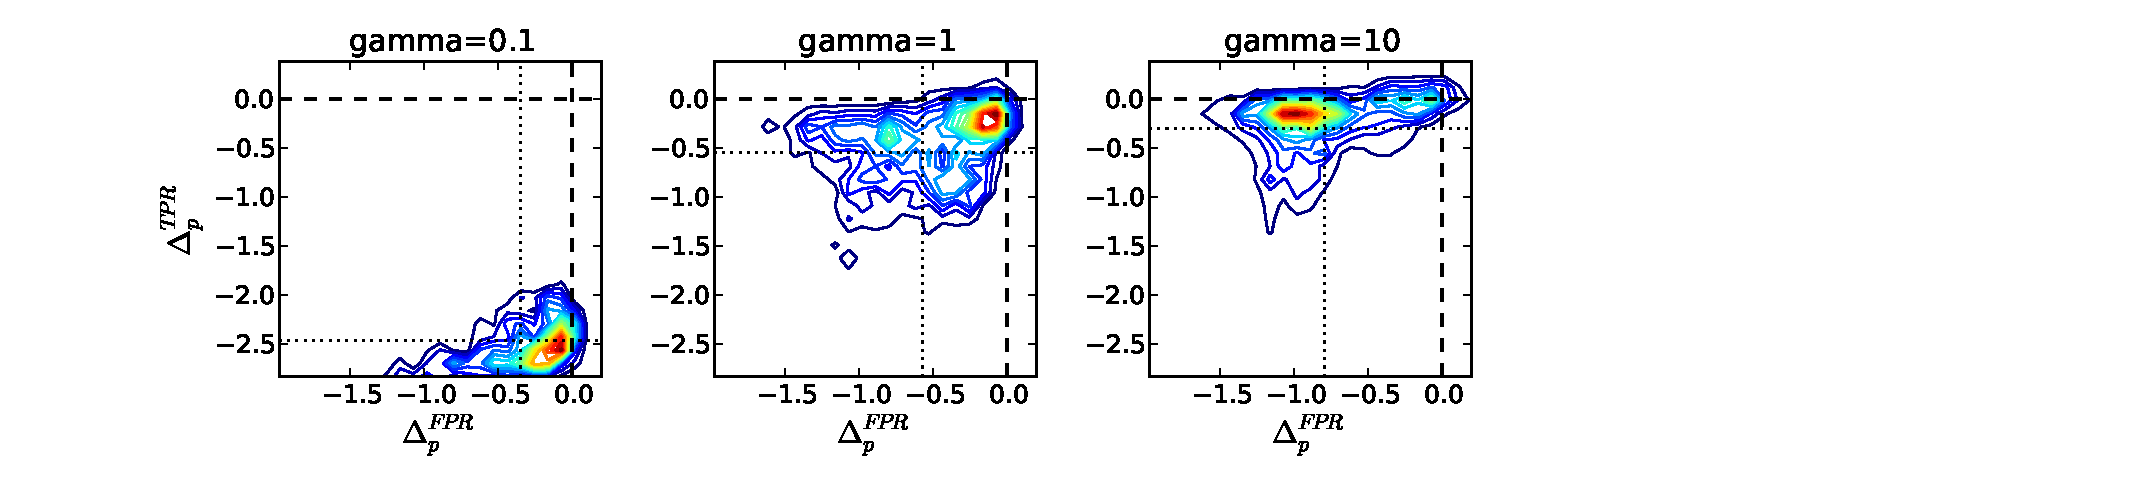
\includegraphics[height=1.5in]{../fig/final/delta_hist_sec/threshold/gamma}
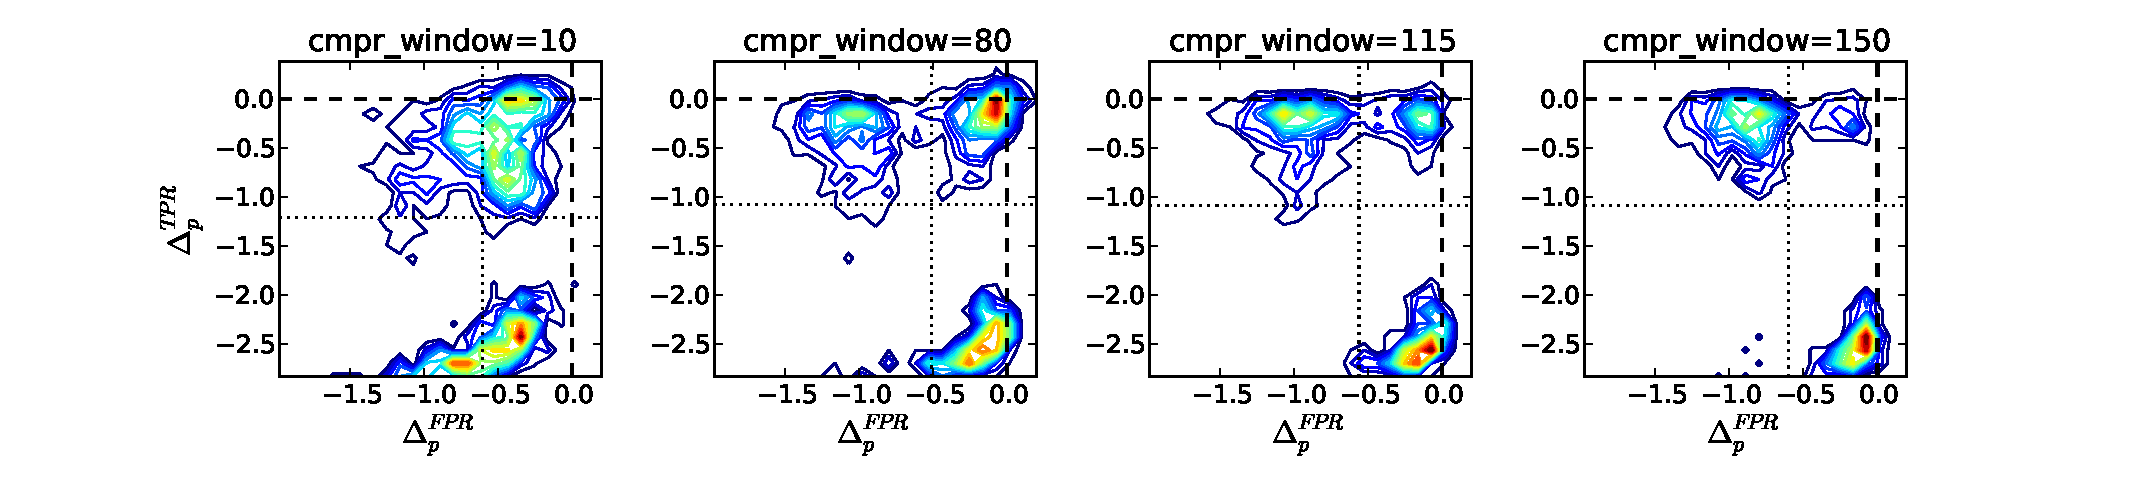
\includegraphics[height=1.5in]{../fig/final/delta_hist_sec/threshold/cmpr_window}
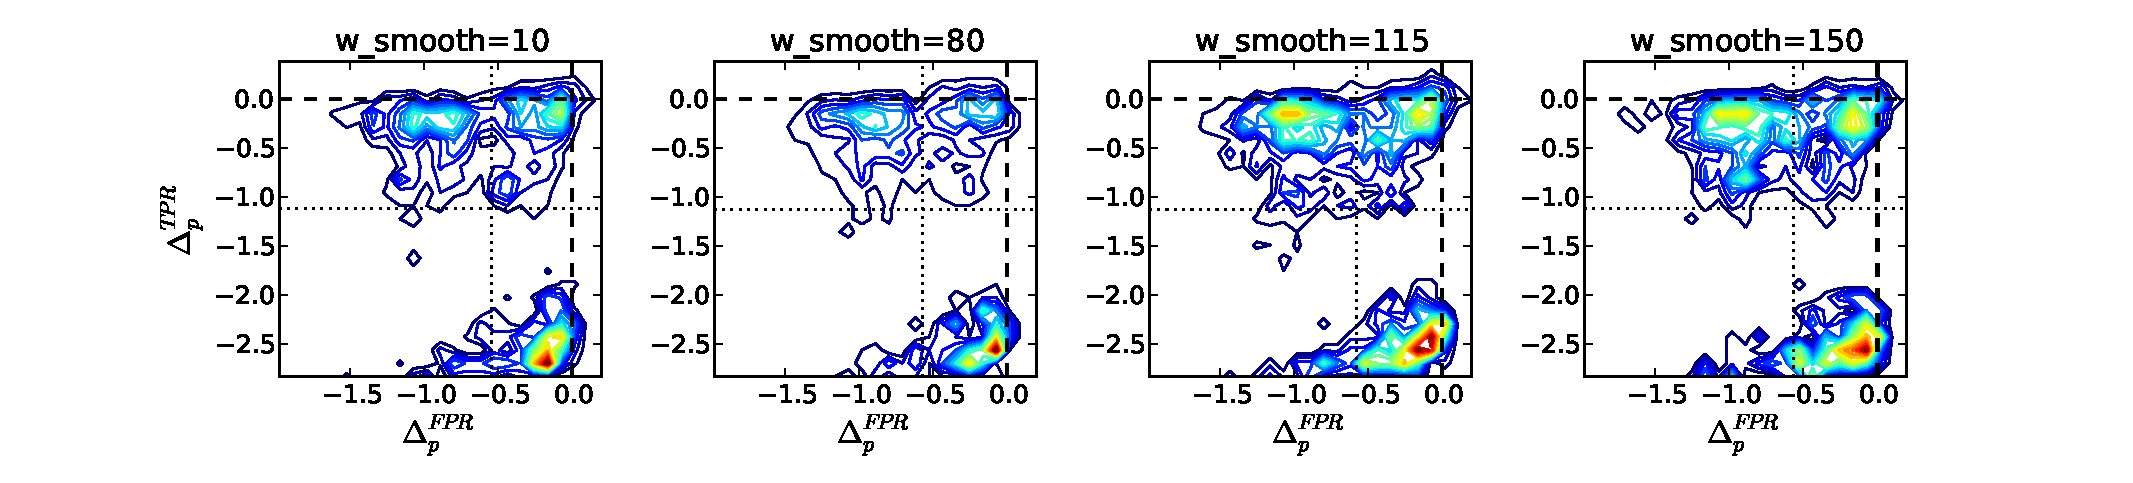
\includegraphics[height=1.5in]{../fig/final/delta_hist_sec/threshold/w_smooth}
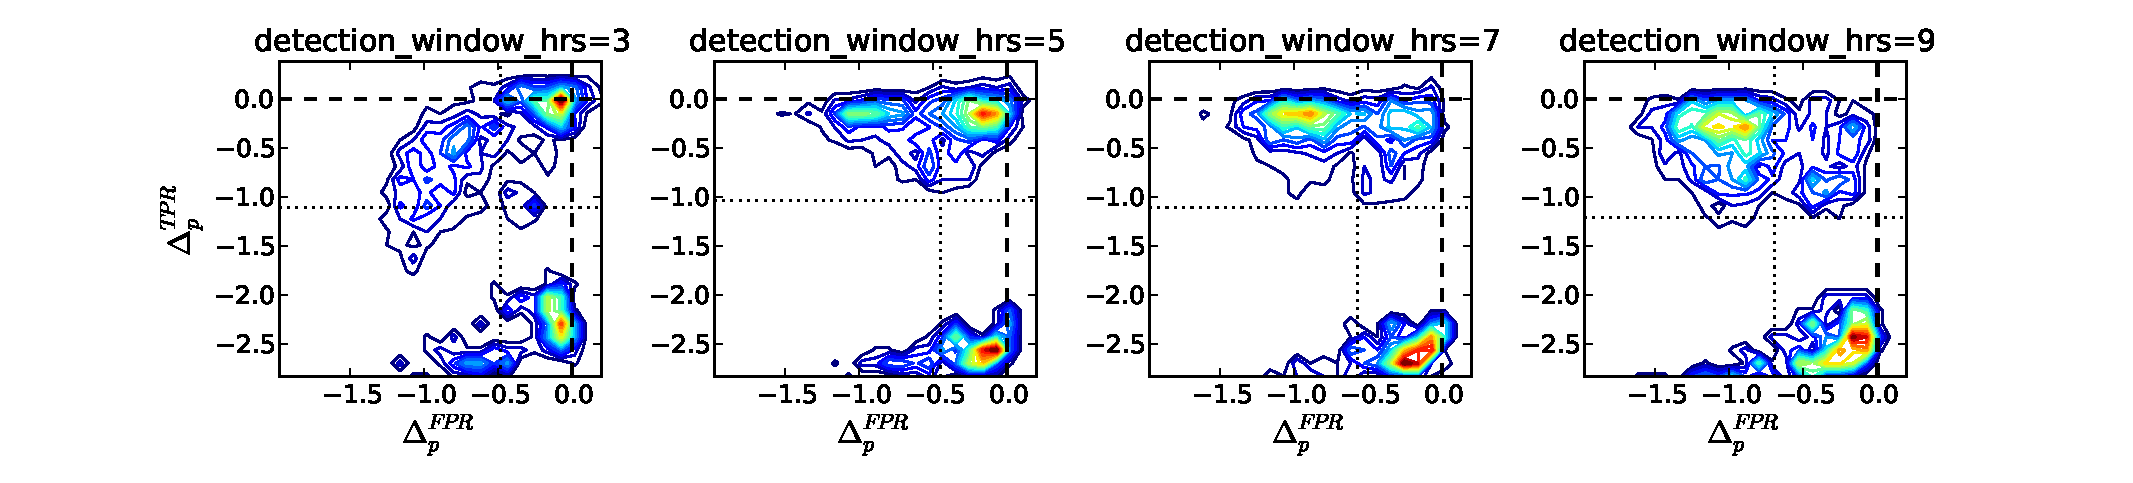
\includegraphics[height=1.5in]{../fig/final/delta_hist_sec/threshold/detection_window_hrs}
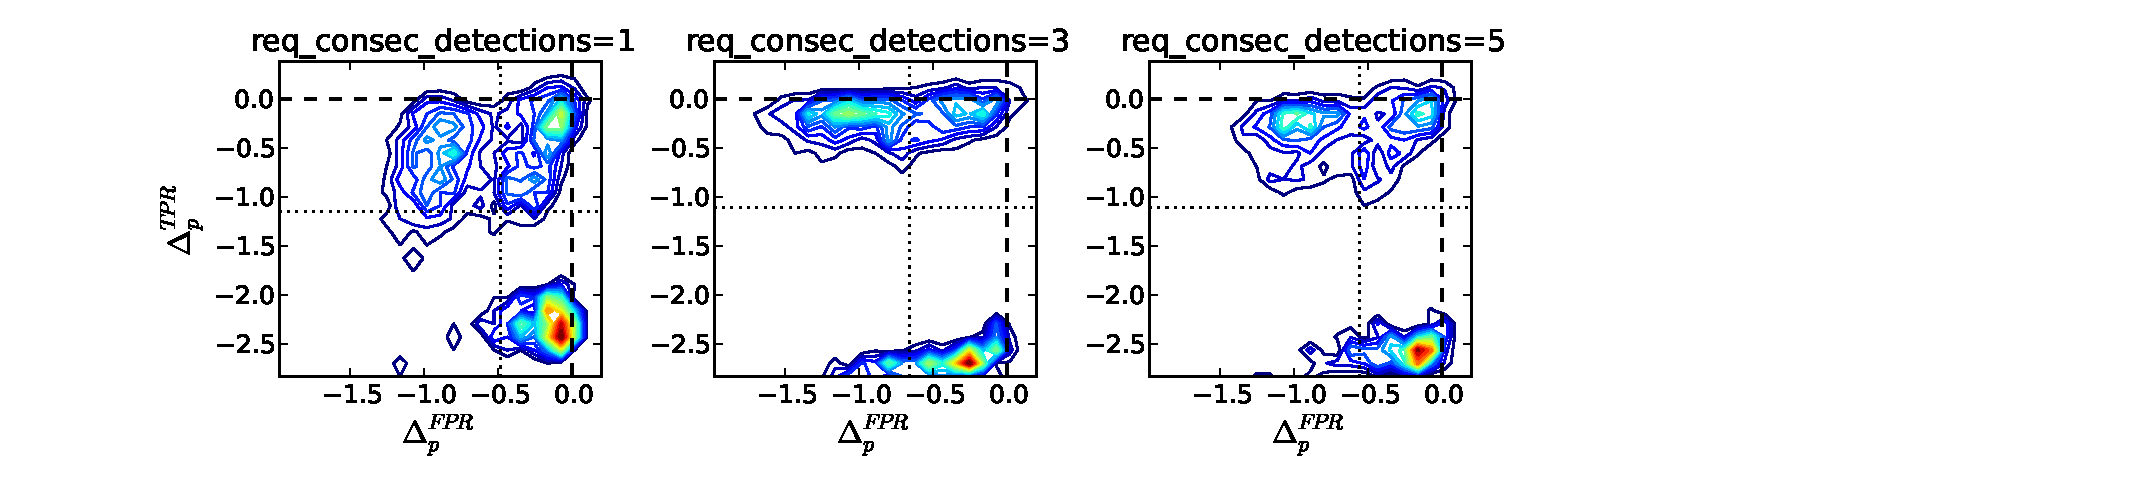
\includegraphics[height=1.5in]{../fig/final/delta_hist_sec/threshold/req_consec_detections}
\end{center}
\caption{\label{fig:delta_sec3} Secondary effects of parameters for a varying \vt{Threshold}}
\end{figure}

\begin{figure}[!h]
\begin{center}
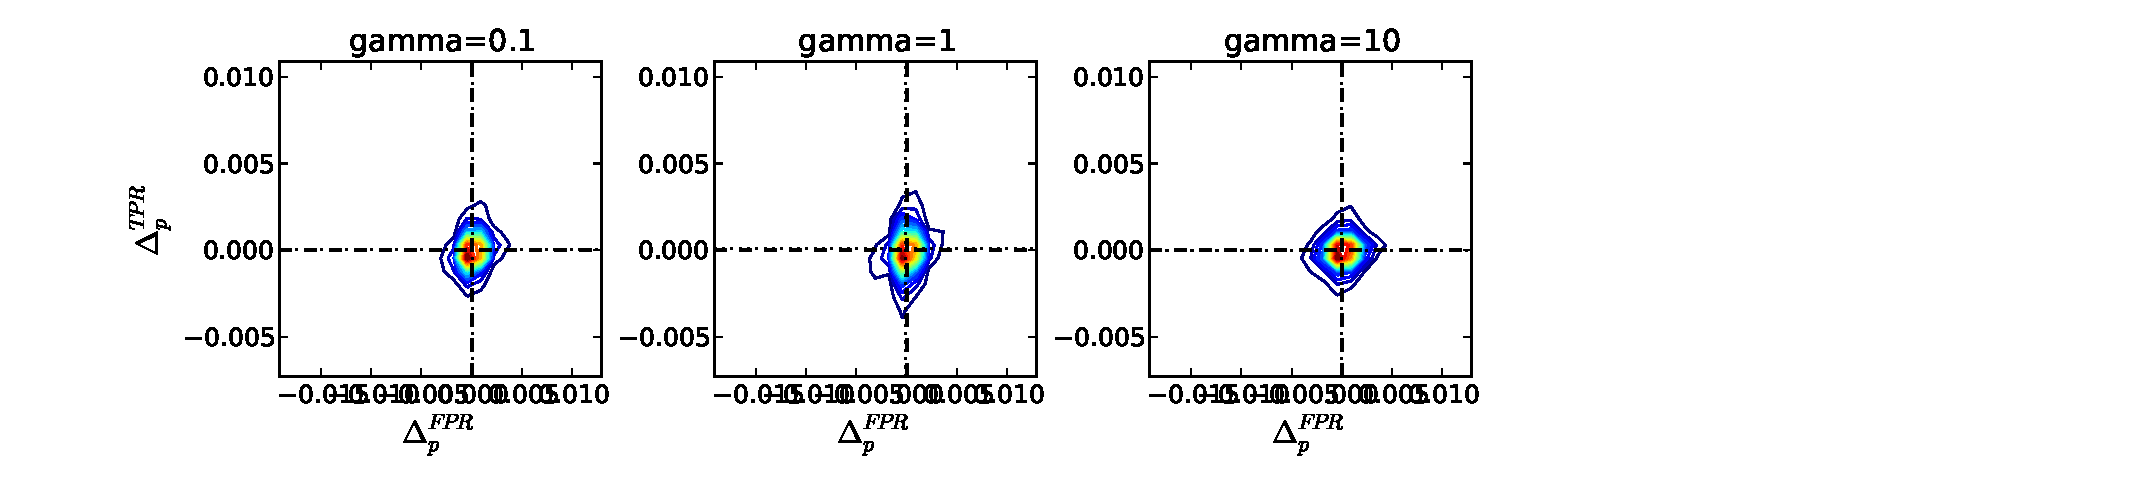
\includegraphics[height=1.5in]{../fig/final/delta_hist_sec/w_smooth/gamma}
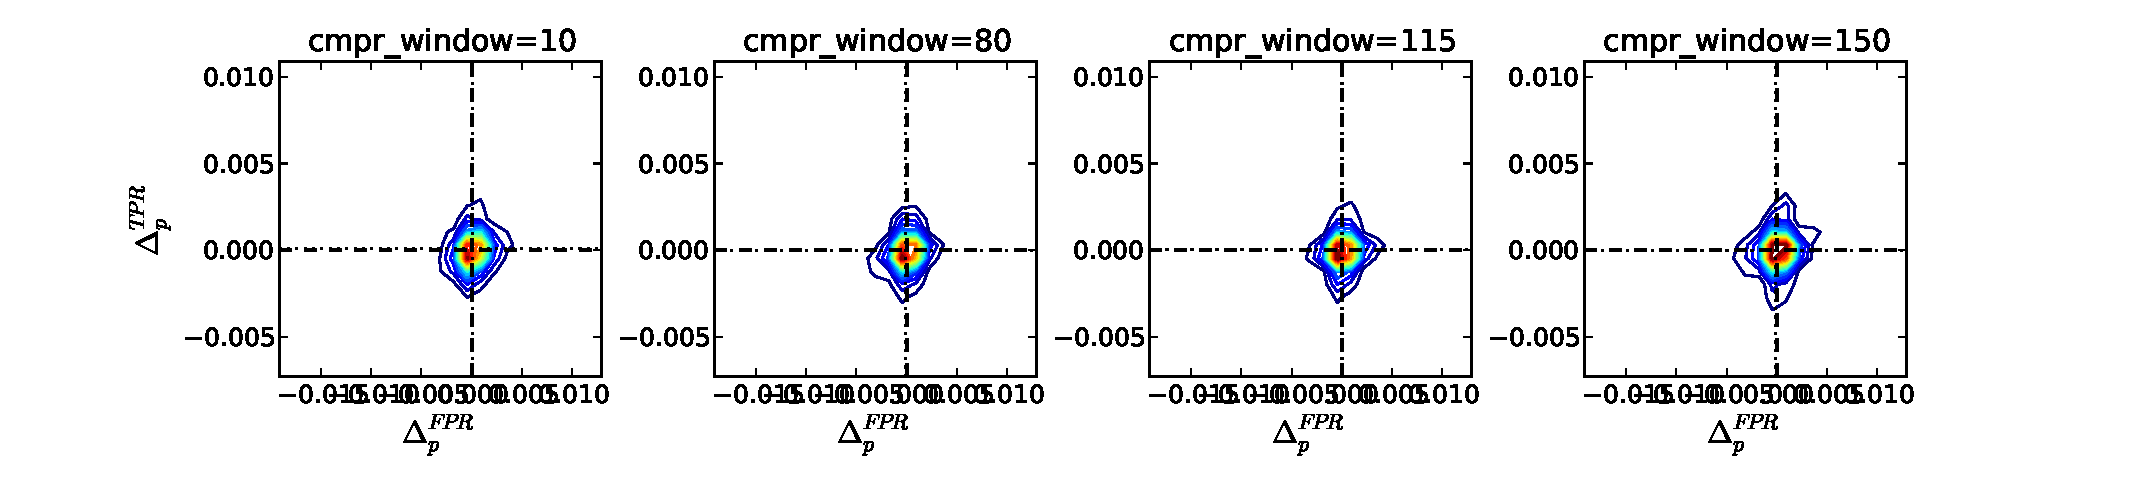
\includegraphics[height=1.5in]{../fig/final/delta_hist_sec/w_smooth/cmpr_window}
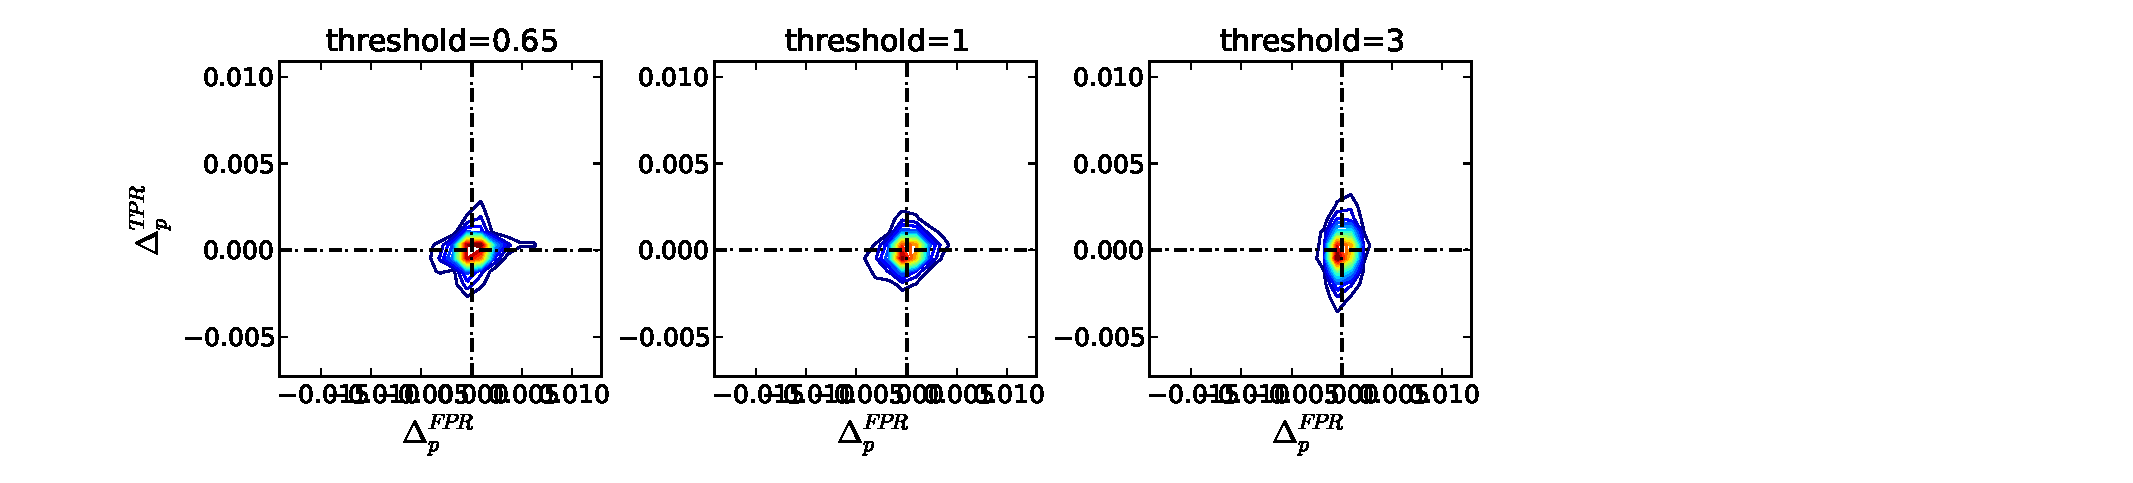
\includegraphics[height=1.5in]{../fig/final/delta_hist_sec/w_smooth/threshold}
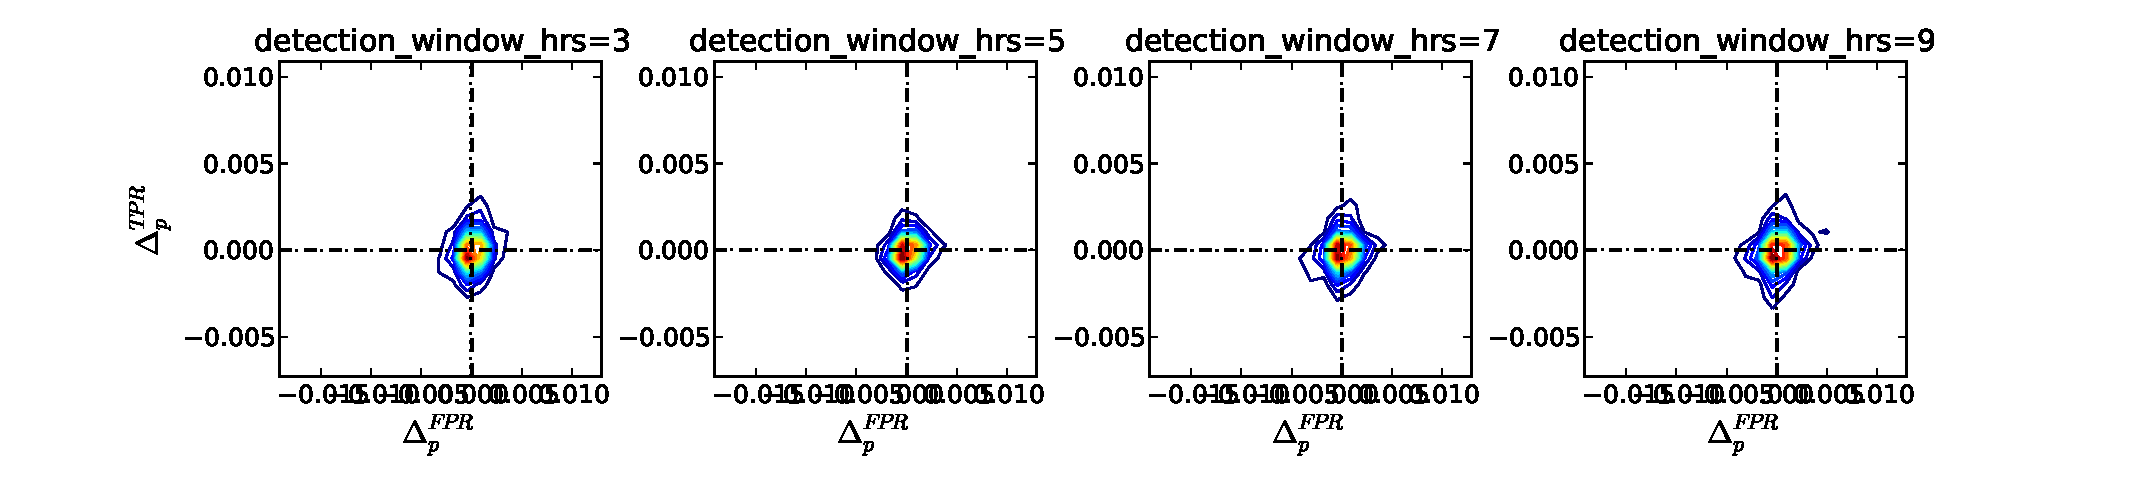
\includegraphics[height=1.5in]{../fig/final/delta_hist_sec/w_smooth/detection_window_hrs}
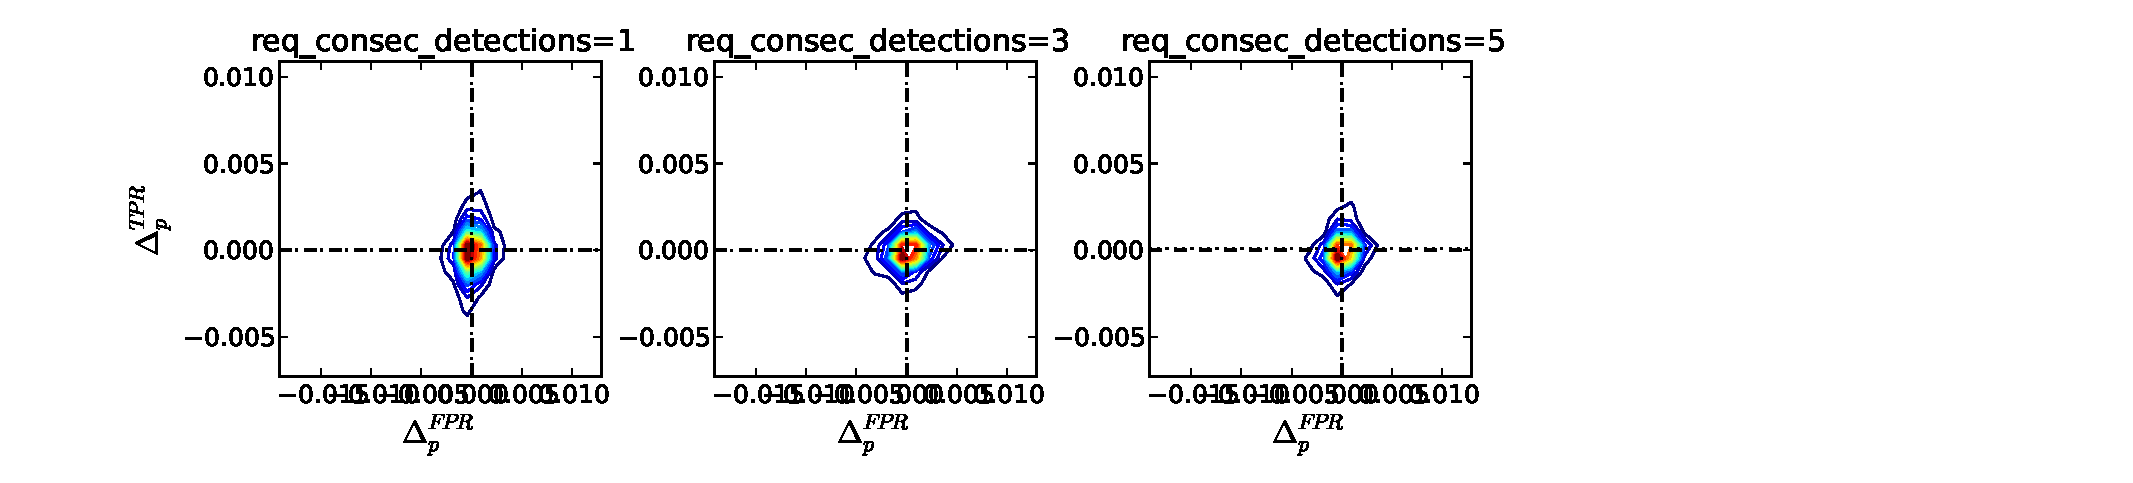
\includegraphics[height=1.5in]{../fig/final/delta_hist_sec/w_smooth/req_consec_detections}
\end{center}
\caption{\label{fig:delta_sec4} Secondary effects of parameters for a varying \vt{WSmooth}}
\end{figure}

\begin{figure}[!h]
\begin{center}
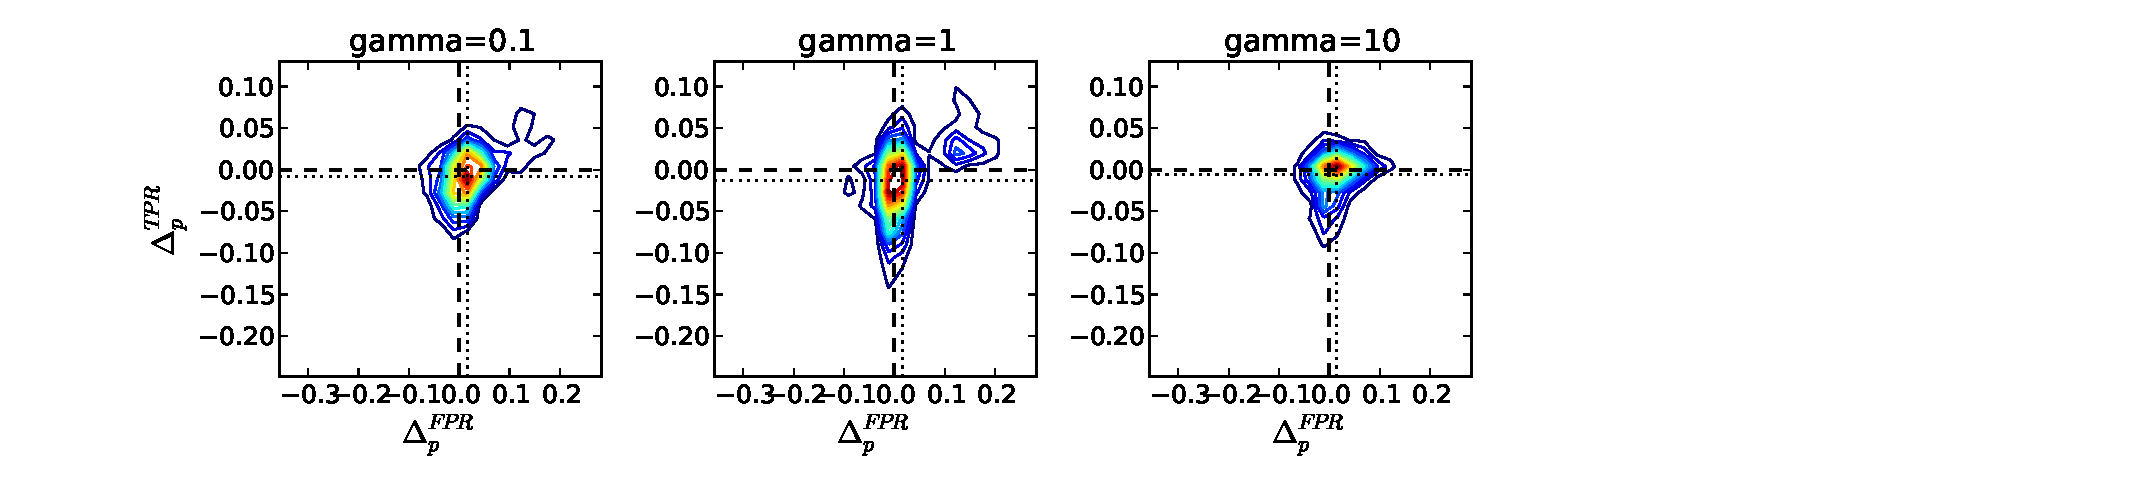
\includegraphics[height=1.5in]{../fig/final/delta_hist_sec/detection_window_hrs/gamma}
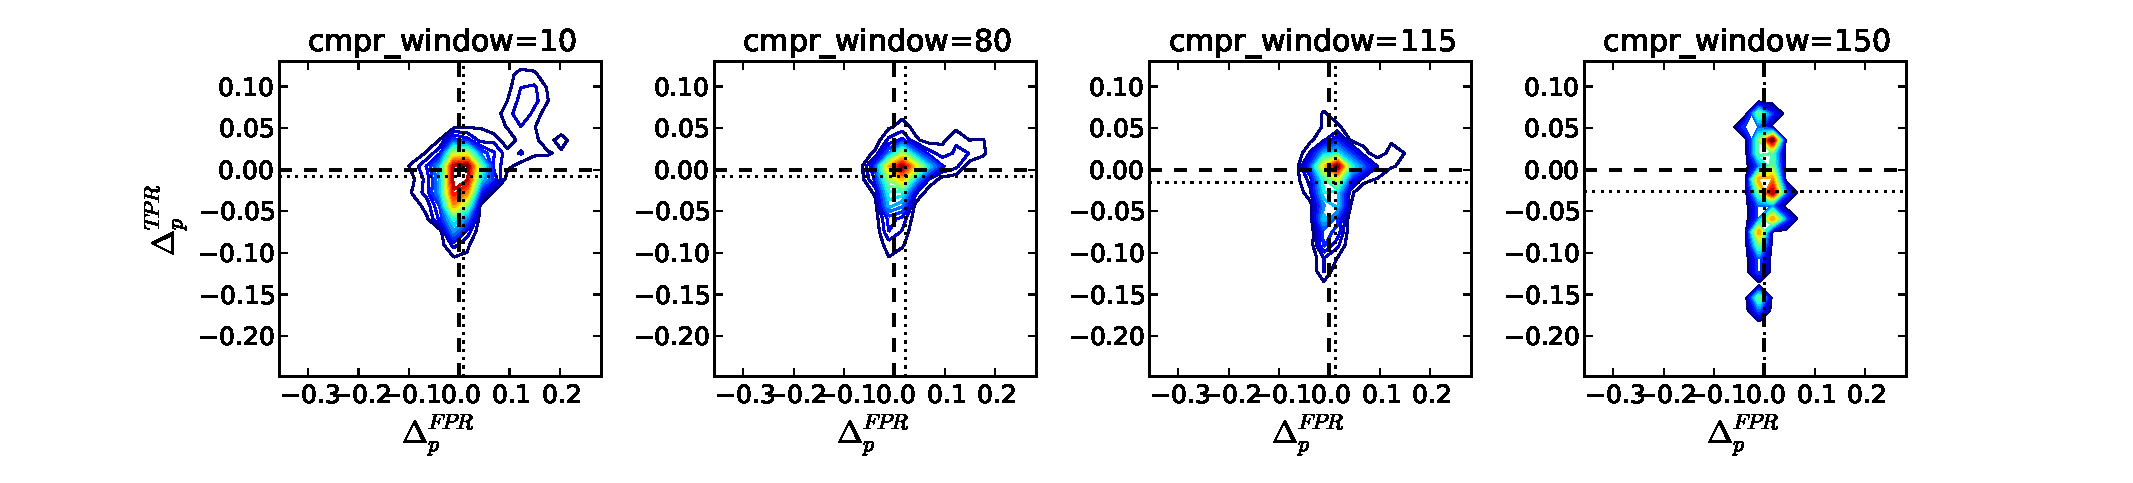
\includegraphics[height=1.5in]{../fig/final/delta_hist_sec/detection_window_hrs/cmpr_window}
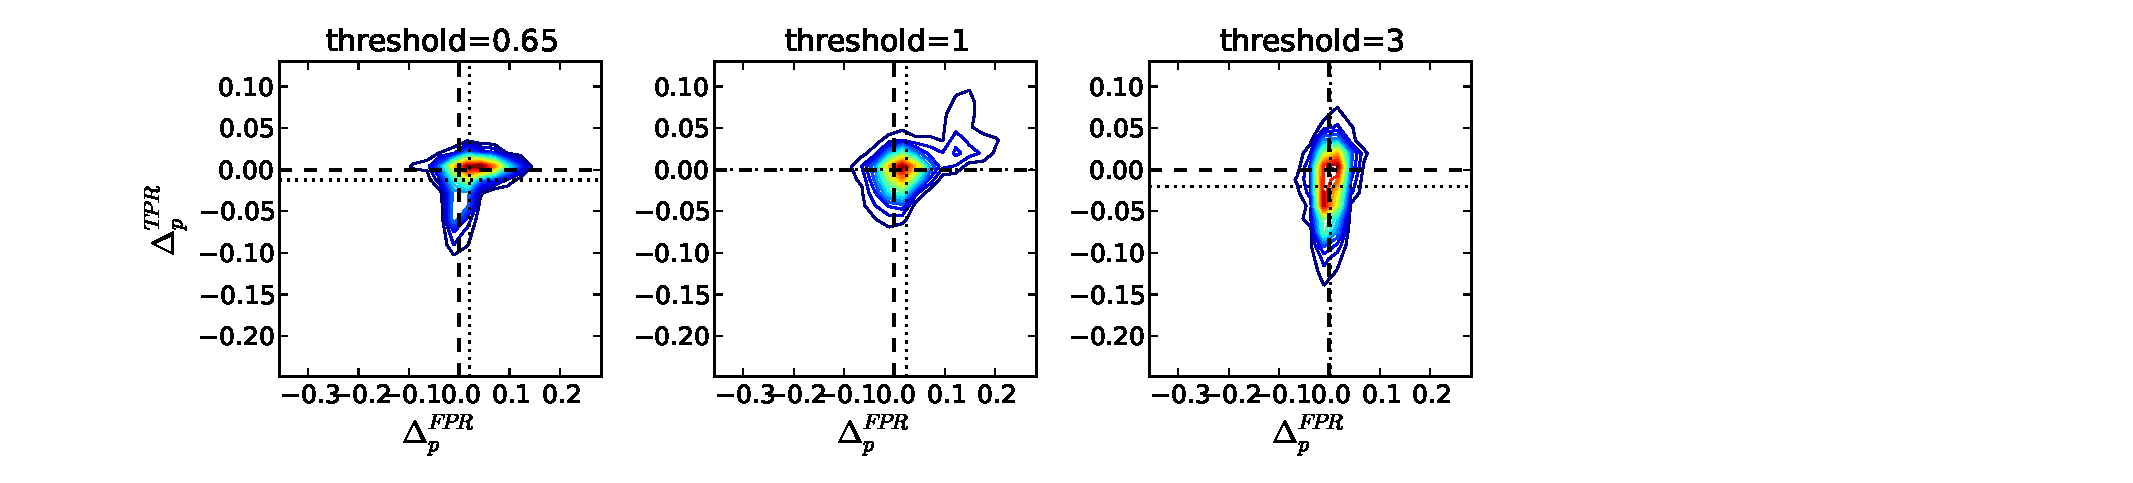
\includegraphics[height=1.5in]{../fig/final/delta_hist_sec/detection_window_hrs/threshold}
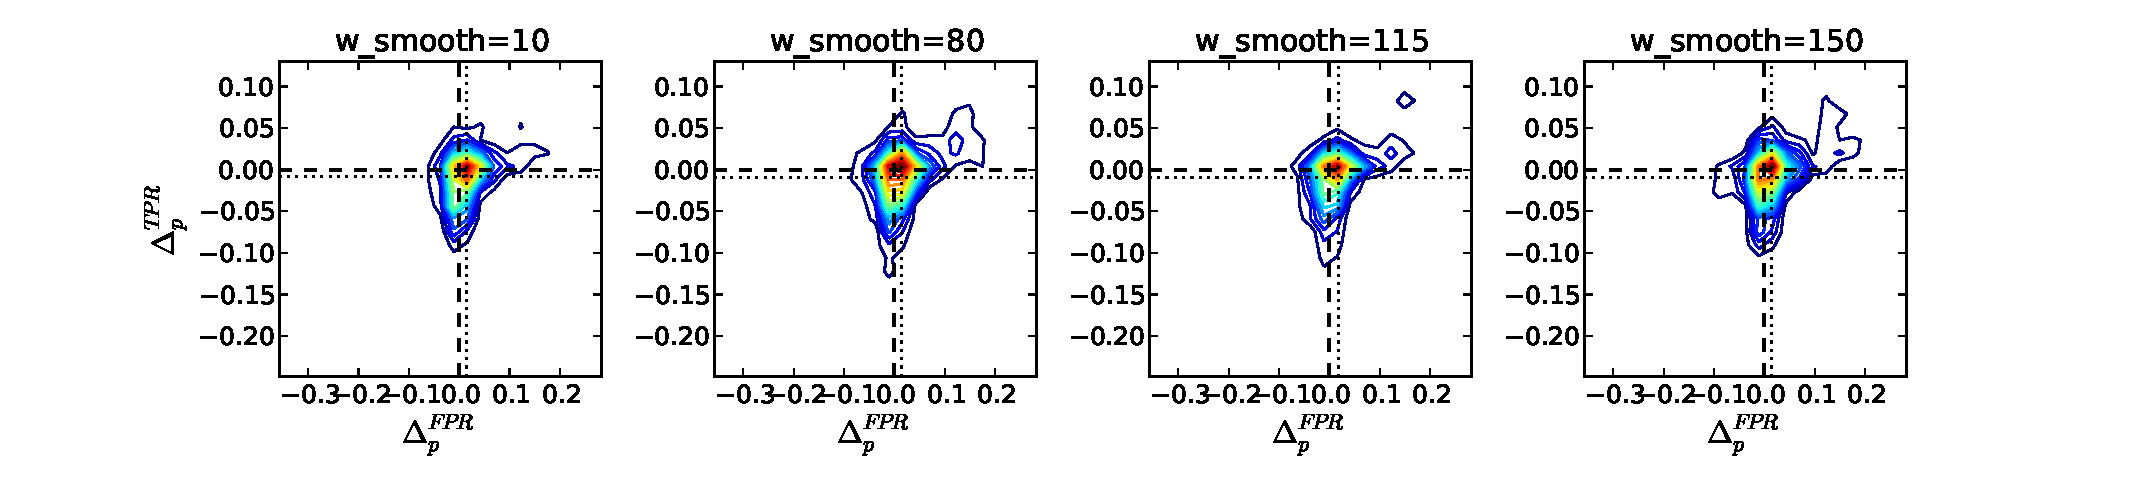
\includegraphics[height=1.5in]{../fig/final/delta_hist_sec/detection_window_hrs/w_smooth}
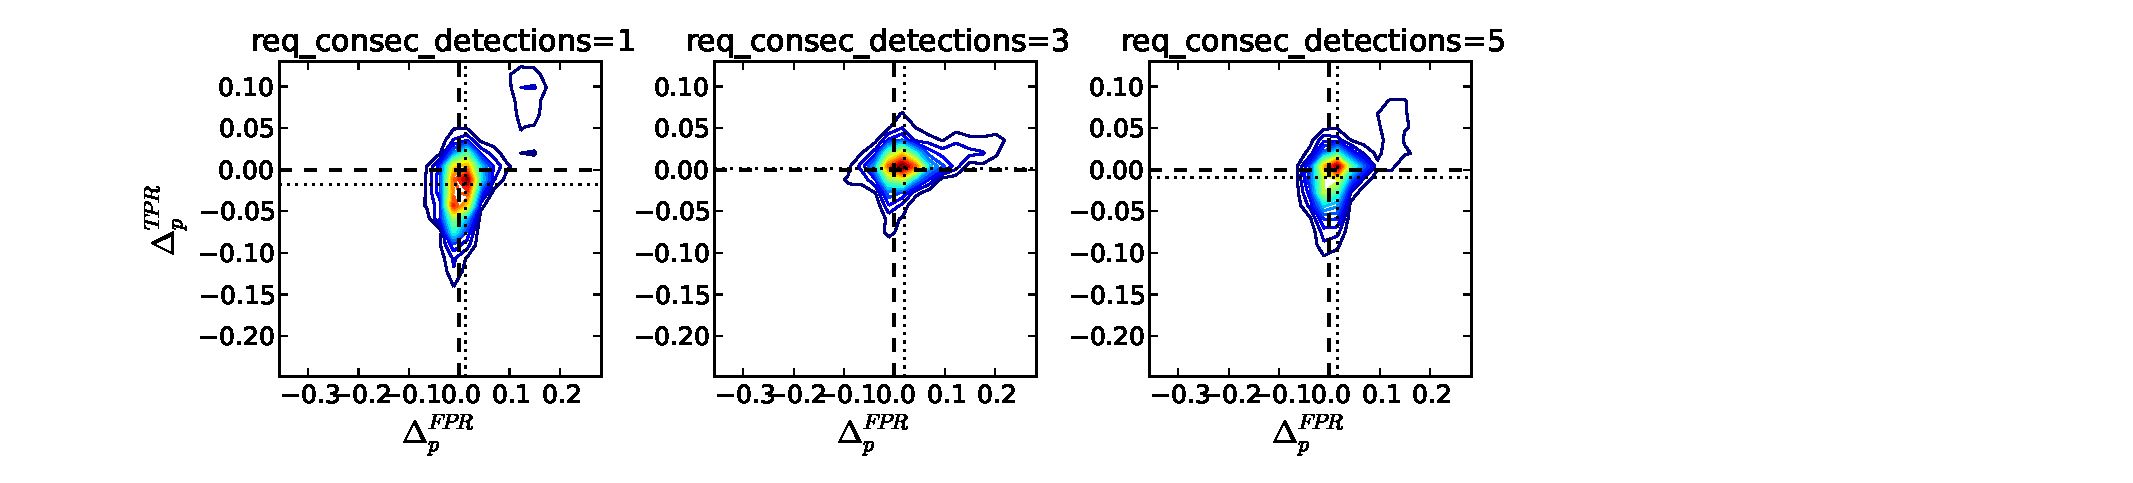
\includegraphics[height=1.5in]{../fig/final/delta_hist_sec/detection_window_hrs/req_consec_detections}
\end{center}
\caption{\label{fig:delta_sec5} Secondary effects of parameters for a varying \vt{DetectionWindowHrs}}
\end{figure}

\begin{figure}[!h]
\begin{center}
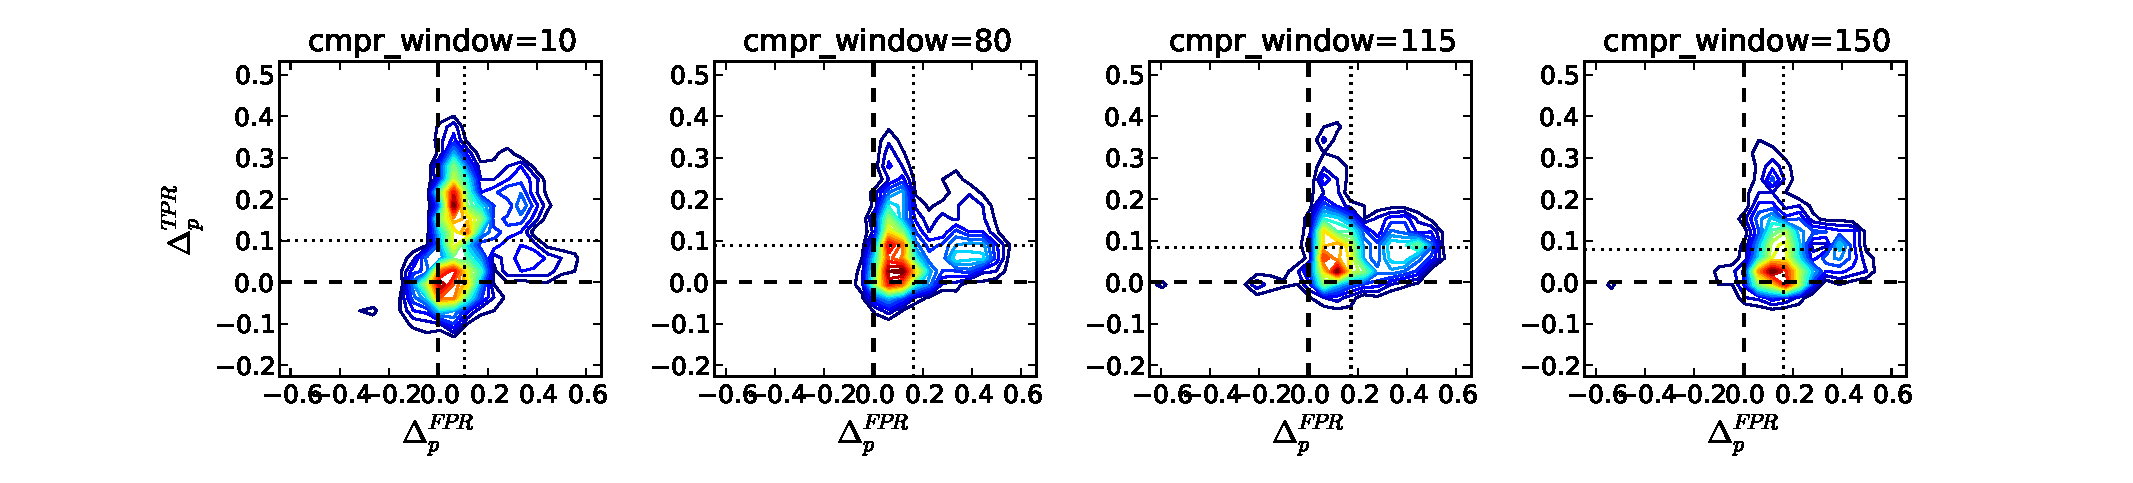
\includegraphics[height=1.5in]{../fig/final/delta_hist_sec/gamma/cmpr_window}
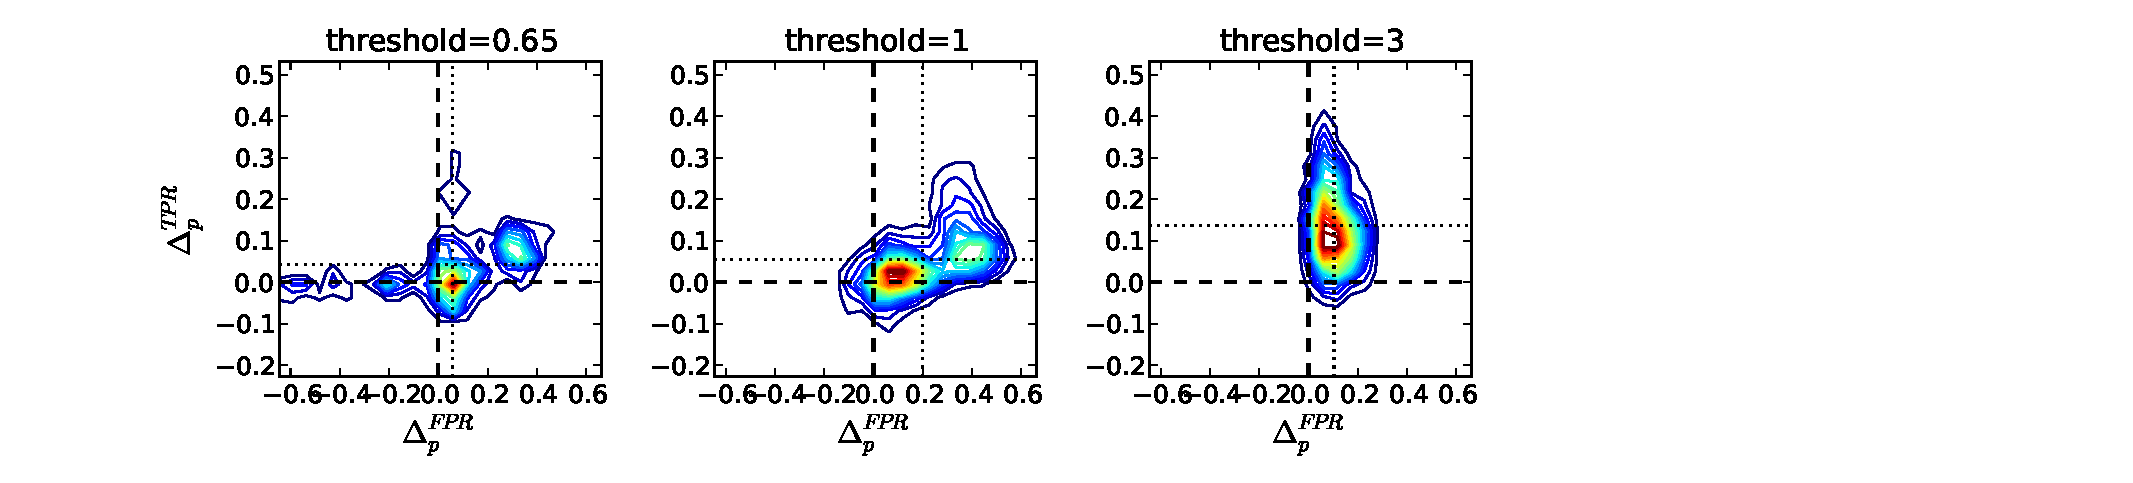
\includegraphics[height=1.5in]{../fig/final/delta_hist_sec/gamma/threshold}
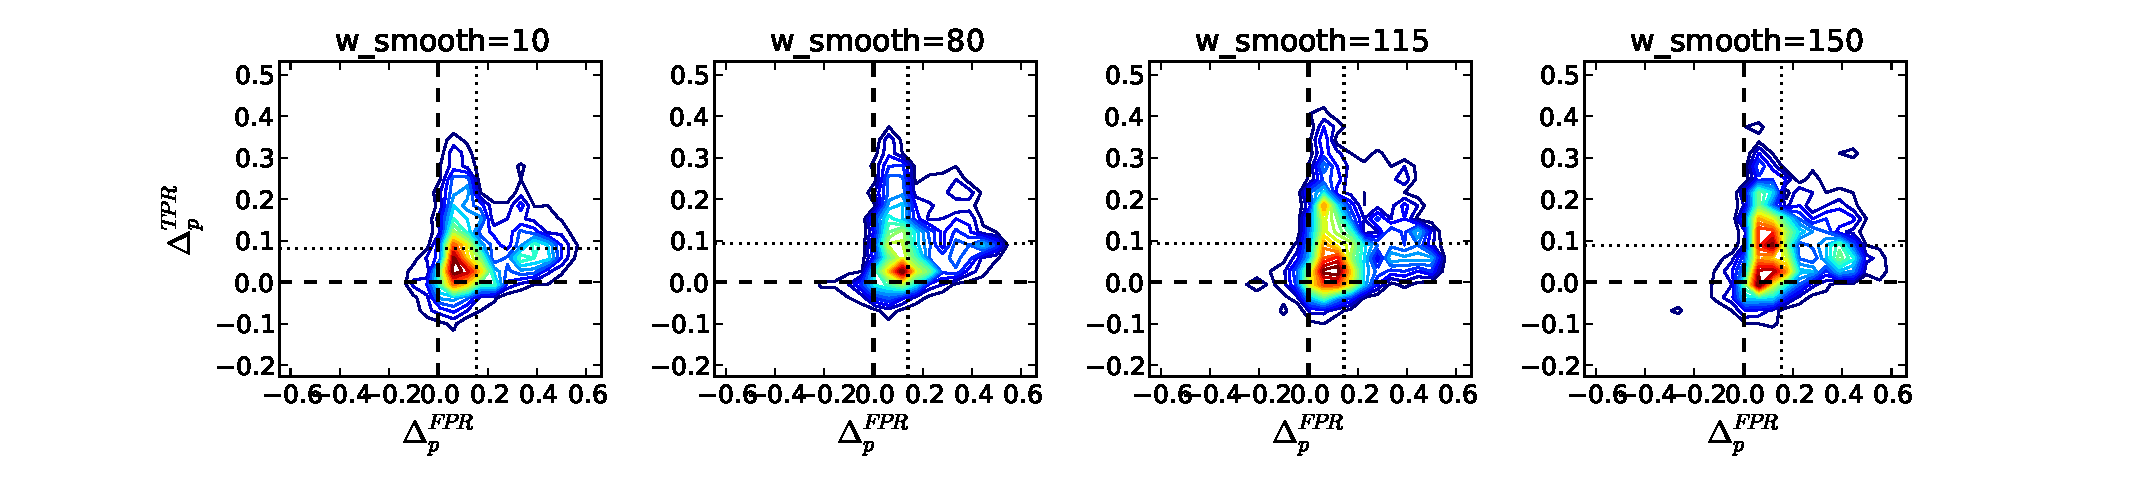
\includegraphics[height=1.5in]{../fig/final/delta_hist_sec/gamma/w_smooth}
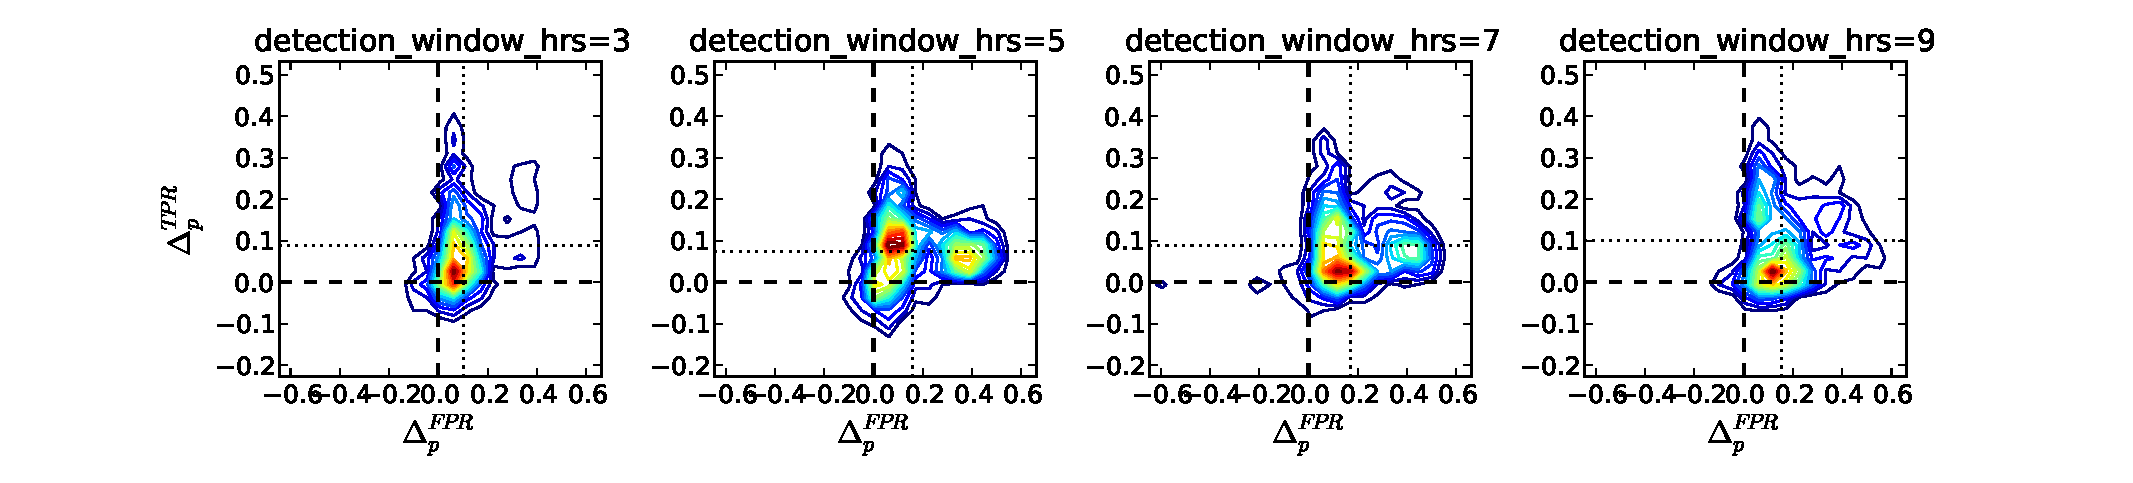
\includegraphics[height=1.5in]{../fig/final/delta_hist_sec/gamma/detection_window_hrs}
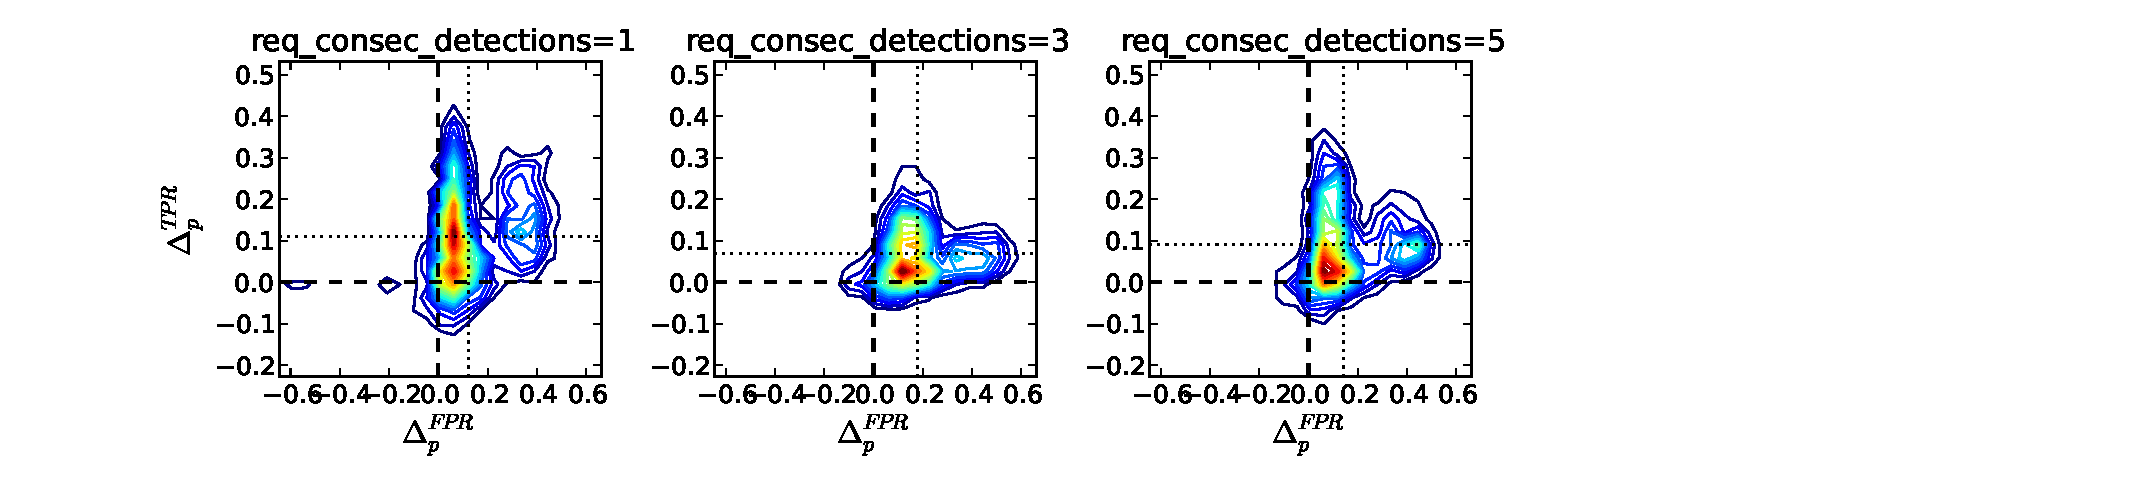
\includegraphics[height=1.5in]{../fig/final/delta_hist_sec/gamma/req_consec_detections}
\end{center}
\caption{\label{fig:delta_sec6} Secondary effects of parameters for a varying \vt{ReqConsecDetections}}
\end{figure}

% Top and bottom ROC curves
Figures that show the top and bottom ROC curves ranked by mean $\Delta_p^{FPR}$ and mean $\Delta_p^{TPR}$.

\begin{figure}[!h]
\begin{center}
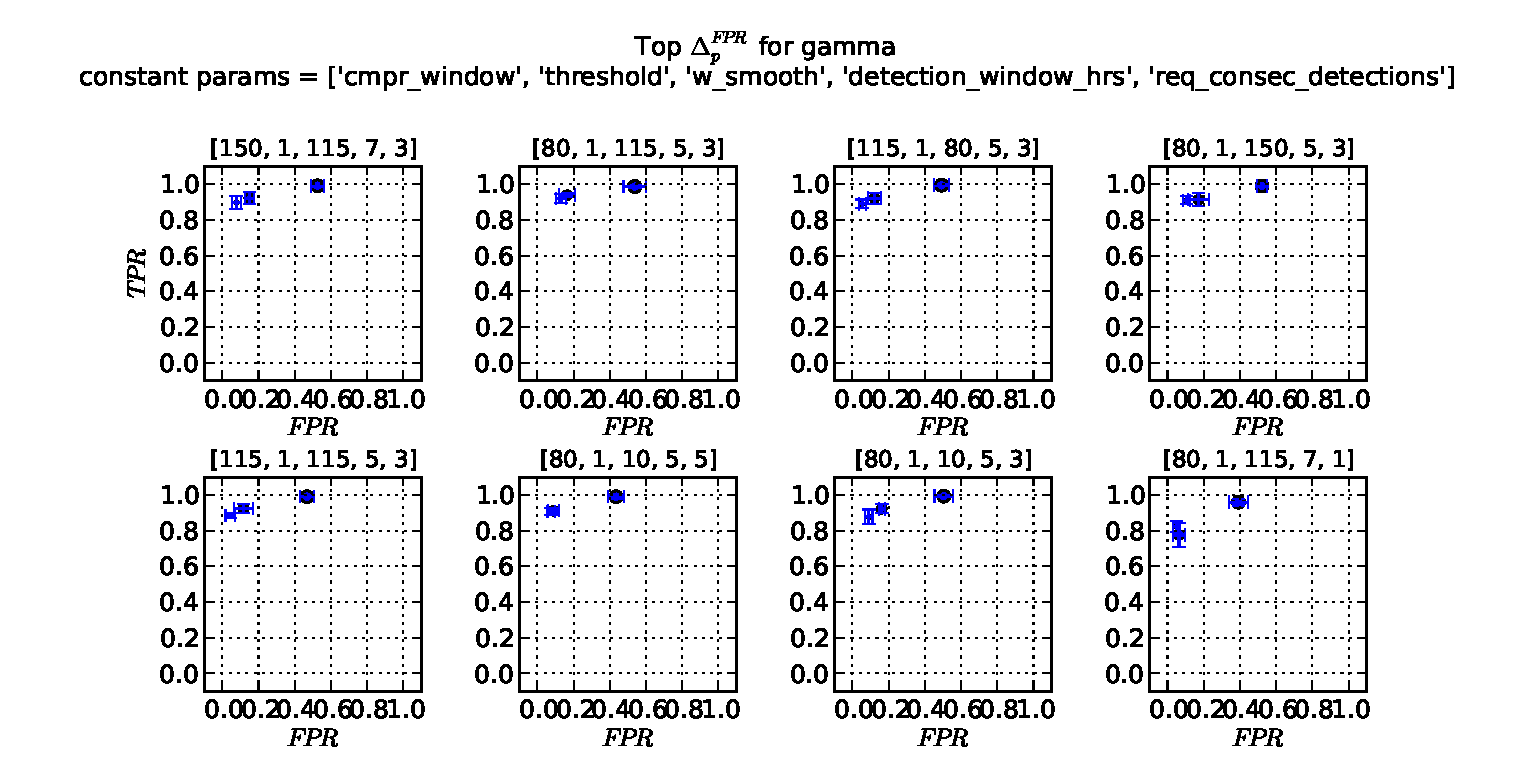
\includegraphics[height=3in]{../fig/final/top_fpr/gamma}
\includegraphics[height=3in]{../fig/final/bottom_fpr/gamma}
\end{center}
\caption{\label{fig:delta_top_bottom1f} Top and bottom $\Delta_p^{FPR}$ for \vt{Gamma}}
\end{figure}


\begin{figure}[!h]
\begin{center}
\includegraphics[height=3in]{../fig/final/top_tpr/gamma}
\includegraphics[height=3in]{../fig/final/bottom_tpr/gamma}
\end{center}
\caption{\label{fig:delta_top_bottom1t} Top and bottom $\Delta_p^{TPR}$ for \vt{Gamma}}
\end{figure}




\begin{figure}[!h]
\begin{center}
\includegraphics[height=3in]{../fig/final/top_fpr/cmpr_window}
\includegraphics[height=3in]{../fig/final/bottom_fpr/cmpr_window}
\end{center}
\caption{\label{fig:delta_top_bottom2f} Top and bottom $\Delta_p^{FPR}$ for \vt{CmprWindow}}
\end{figure}

\begin{figure}[!h]
\begin{center}
\includegraphics[height=3in]{../fig/final/top_tpr/cmpr_window}
\includegraphics[height=3in]{../fig/final/bottom_tpr/cmpr_window}
\end{center}
\caption{\label{fig:delta_top_bottom2t} Top and bottom $\Delta_p^{TPR}$ for \vt{CmprWindow}}
\end{figure}



% Threshold
\begin{figure}[!h]
\begin{center}
\includegraphics[height=3in]{../fig/final/top_fpr/threshold}
\includegraphics[height=3in]{../fig/final/bottom_fpr/threshold}
\end{center}
\caption{\label{fig:delta_top_bottom3f} Top and bottom $\Delta_p^{FPR}$ for \vt{Threshold}}
\end{figure}


\begin{figure}[!h]
\begin{center}
\includegraphics[height=3in]{../fig/final/top_tpr/threshold}
\includegraphics[height=3in]{../fig/final/bottom_tpr/threshold}
\end{center}
\caption{\label{fig:delta_top_bottom3t} Top and bottom $\Delta_p^{TPR}$ for \vt{Threshold}}
\end{figure}



% WSmooth
\begin{figure}[!h]
\begin{center}
\includegraphics[height=3in]{../fig/final/top_fpr/w_smooth}
\includegraphics[height=3in]{../fig/final/bottom_fpr/w_smooth}
\end{center}
\caption{\label{fig:delta_top_bottom4f} Top and bottom $\Delta_p^{FPR}$ for \vt{WSmooth}}
\end{figure}

\begin{figure}[!h]
\begin{center}
\includegraphics[height=3in]{../fig/final/top_tpr/w_smooth}
\includegraphics[height=3in]{../fig/final/bottom_tpr/w_smooth}
\end{center}
\caption{\label{fig:delta_top_bottom4t} Top and bottom $\Delta_p^{TPR}$ for \vt{WSmooth}}
\end{figure}


% DetectionWindowHrs
\begin{figure}[!h]
\begin{center}
\includegraphics[height=3in]{../fig/final/top_fpr/detection_window_hrs}
\includegraphics[height=3in]{../fig/final/bottom_fpr/detection_window_hrs}
\end{center}
\caption{\label{fig:delta_top_bottom5f} Top and bottom $\Delta_p^{FPR}$ for \vt{DetectionWindowHrs}}
\end{figure}

\begin{figure}[!h]
\begin{center}
\includegraphics[height=3in]{../fig/final/top_tpr/detection_window_hrs}
\includegraphics[height=3in]{../fig/final/bottom_tpr/detection_window_hrs}
\end{center}
\caption{\label{fig:delta_top_bottom5t} Top and bottom $\Delta_p^{TPR}$ for \vt{DetectionWindowHrs}}
\end{figure}

% ReqConsecDetections
\begin{figure}[!h]
\begin{center}
\includegraphics[height=3in]{../fig/final/top_fpr/req_consec_detections}
\includegraphics[height=3in]{../fig/final/bottom_fpr/req_consec_detections}
\end{center}
\caption{\label{fig:delta_top_bottom6f} Top and bottom $\Delta_p^{FPR}$ for \vt{ReqConsecDetections}}
\end{figure}

\begin{figure}[!h]
\begin{center}
\includegraphics[height=3in]{../fig/final/top_tpr/req_consec_detections}
\includegraphics[height=3in]{../fig/final/bottom_tpr/req_consec_detections}
\end{center}
\caption{\label{fig:delta_top_bottom6t} Top and bottom $\Delta_p^{TPR}$ for \vt{ReqConsecDetections}}
\end{figure}

% TODO: Discuss effect on relative detection time

%TODO: Ranking of all combinations of fixed parameters based on tpr (and based
%on fpr). Show many (ranked) thumbnail ROC curves for each varying parameter.

%TODO: Ranking of all combinations of fixed parameters based on pct(deltas >
%0). Restrict to the important params and show delta histograms again, showing a
%consistent up or down movement along the curve. Show many (ranked) thumbnail
%ROC curves for each varying parameter.

% Wait a minute... if varying a parameter moves TPR up and FPR down, isn't
% that... really really good?
\section{Recommendations}

\chapter{Summary of Contributions and Future Work}
\label{ch:conclusion}

\section{Contributions}
We have introduced a setting to do inference in the presence of large amounts of
data governed by an underlying stochastic model. Within this setting, we have
derived an online time series classification method and an associated
implementation that is simple, efficient, and scalable. To investigat the
classification performance of our method, we applied it to the task of
predicting trending topics on Twitter. We showed the method's flexibility by
analyzing the effects of the algorithm parameters, and quantified the tradeoffs
between relative detection time, true positive rate, and false positive
rate. Finally, we demonstrated the method to be succesful in predicting trending
topics on Twitter, at a low error rate, often before they are detected by
Twitter.

\section{Future Work}
Possible directions for future work include the following:

\begin{itemize}
\item To take advantage of the structure in large amounts of unlabeled data, it
  would be desirable to extend the theory and algorithms presented in this
  thesis to handle large amounts of unlabeled data.
\item I'm going to think about this some more. I am still struggling a bit with
  the big picture view. If you think of something, please let me know.
\end{itemize}


\appendix
%%% This defines the bibliography file (main.bib) and the bibliography style.
%% If you want to create a bibliography file by hand, change the contents of
%% this file to a `thebibliography' environment.  For more information 
%% see section 4.3 of the LaTeX manual.
\begin{singlespace}
\bibliography{main}
\bibliographystyle{plain}
\end{singlespace}

\end{document}

